
%%==================================================
%% demo.tex for BIT Thesis
%% modified by yang yating
%% version: 1.2
%% last update: Jan. 4th, 2018
%%==================================================

% 默认单面打印 oneside 、硕士论文模板 master

\documentclass[oneside, doctor]{BIT-thesis-grd}
\newtheorem{definition}{定义}
\usepackage{algorithm}
\usepackage{algorithmic}

% 模板选项: 硕士论文 master; 博士论文 doctor

%==============更改数学字体设置,Latin Modern Math 默认的的确有点细,看个人需要,下面提供一种方法,需要的可以取消注释=========%

% \usepackage[bold-style=ISO]{unicode-math} %采用unicode-math,可以直接输入Unicode公式,当然传统的输入就行
% \setmathfont{XITS Math}  %目前unicode-math 支持几种数学字体,具体用法可以查看帮助文档,这里采用类似times字体科学数学字体,可以取消注释对比


\begin{document}

%%%%%%%%%%%%%%%%%%%%%%%%%%%%%%
%% 封面
%%%%%%%%%%%%%%%%%%%%%%%%%%%%%%

% 中文封面内容(关注内容而不是表现形式)
\classification{TP391.1}
\UDC{004.8}

\title{事件抽取中的共性数据依赖研究}
\vtitle{事件抽取中的共性数据依赖研究}
\author{***}
\institute{计算机学院}
\advisor{****}
\chairman{****}
\degree{工学博士}
\major{计算机科学与技术}
\school{北京理工大学}
\defenddate{2024年6月}
%\studentnumber{**********}


% 英文封面内容(关注内容而不是表现形式)
\englishtitle{Research on Common Data Dependency in Event Extraction}
\englishauthor{***}
\englishadvisor{****}
\englishchairman{****}
\englishschool{Beijing Institute of Technology}
\englishinstitute{School of Computer Science}
\englishdegree{Doctor of Philosophy}
\englishmajor{Computer Science and Technology}
\englishdate{June, 2024}

% 封面绘制
\maketitle

% 中文信息
\makeInfo

% 英文信息
\makeEnglishInfo

%打印竖排论文题目
\makeVerticalTitle

% 论文原创性声明和使用授权
\makeDeclareOriginal

%%%%%%%%%%%%%%%%%%%%%%%%%%%%%%
%% 前置部分
%%%%%%%%%%%%%%%%%%%%%%%%%%%%%%
\frontmatter

% 摘要
%%==================================================
%% abstract.tex for BIT Master Thesis
%% modified by yang yating
%% version: 0.1
%% last update: Dec 25th, 2016
%%==================================================

\begin{abstract}
事件抽取作为信息抽取领域的关键组成部分,其提供的结构化语义信息广泛应用在事实核查、信息检索、智能问答、推荐系统等多样化自然语言场景中。此外,以事件抽取为基础构建的事件知识图谱同样具备了广阔的应用前景。随着深度学习技术的快速发展,现有方法利用特定神经网络架构研究事件抽取的不同阶段任务。尽管这些方法取得了优异的性能进步,仍存在如下的共性数据挑战:1)不同事件检测方法存在的数据不平衡依赖,限制了其识别事件的能力,进一步降低了整体检测性能;2)不同事件要素抽取方法存在的实体类型过度依赖,阻碍了其学习实体类型以外的更多语义信息,影响了事件要素类型的正确预测;3)当事件要素抽取任务扩展到多级别文本时,不同事件要素抽取方法存在的内在局限和跨事件信息限制,阻碍了其从不同级别文本中有效构建跨事件依赖关系,限制了多事件的要素抽取能力。为此,本文围绕事件抽取中的共性数据依赖展开研究,主要研究内容和创新成果如下:

(1)提出基于分类器自适应知识蒸馏的数据不平衡依赖消解方法。针对事件检测中存在的数据不平衡依赖,首先研究其影响事件检测性能的方式,并相应定义和引入句子级别识别信息,以主动消解数据不平衡依赖导致的性能损失。在此基础上,提出一种基于分类器自适应知识蒸馏的事件检测方法。具体地,该方法在事件识别增强网络中引入根据训练实例标签转化的句子级别识别信息,并将其作为输入的一部分参与训练。进一步,设计额外的训练任务,通过事件识别增强网络的分类器引导事件检测网络从原始文本中自动学习句子级别识别信息,从而实现事件检测性能的提升。实验评估表明,提出的方法可以通用有效地消解数据不平衡依赖对于不同事件检测模型的性能影响,并展现自主适应不同程度数据不平衡和跨任务扩展的能力。

(2)提出基于多角度对比学习的实体类型过度依赖消解方法。针对事件要素抽取中存在的实体类型过度依赖,首先定义并研究该依赖在不同事件要素抽取模型架构中的存在性。在此基础上,提出一种基于多角度对比学习的事件要素抽取方法。具体地,构建两个监督对比学习模块,在正样本角度提升具有相同要素类型但具有不同实体类型的实例特征表示间的相似性,而在负样本角度降低具有不同要素类型但具有相同实体类型的实例特征表示间的相似性。进一步,设计循环训练策略提升多角度消解的效率。实验评估表明,提出的方法可以通用有效地消解不同事件要素抽取架构的实体类型过度依赖,并基于预训练语言模型架构取得当前最优性能。

(3)提出基于分离-融合范式的跨事件信息构建与利用方法。首先总结目前通用文本级别事件要素抽取方法存在的内在局限,提出基于多词元链接的建模方法。进一步,为了从不同级别文本中高效利用跨事件依赖信息,提出分离-融合抽取范式,其将跨事件信息获取和事件要素抽取先分开建模再进行融合,从而充分利用不同抽取范式的优势。遵循该范式,提出一种新的多词元链接模型。具体地,引入一个链接模块连接不同事件的触发词和对应的要素类型以提供跨事件信息,同时构建另一个链接模块抽取目标事件的要素信息。此外,提出一个两阶段融合模块将获取的跨事件信息融合到目标事件的要素抽取中。实验结果表明,提出的方法在不同的句子级别和文档级别数据集上均显著超越目前性能最优的事件要素抽取基线。

本文面向事件抽取系统中的数据不平衡依赖、实体类型过度依赖和
跨事件依赖三类共性数据挑战,相应研究分类器自适应知识蒸馏、多角度对比学习和分离-融合范式三种通用性方法,覆盖不同模型架构、不同文本范围和不同事件抽取阶段,以有力提升语言智能化和事件知识图谱构建自动化水平。

\keywords{事件抽取; 共性数据依赖; 数据不平衡依赖; 实体类型过度依赖; 跨事件依赖}
\end{abstract}

\begin{englishabstract}

As a key component in information extraction, event extraction provides structured semantic information that is widely used in diverse natural language scenarios such as fact checking, information retrieval, intelligent question answering, and recommendation systems. In addition, the event knowledge graph based on event extraction also holds broad application prospects. With the rapid development of deep learning technology, existing methods use specific neural network architectures to study different stages of event extraction. Although these methods have made excellent performance progress, there are still the following common data challenges: 1) The data imbalance dependency in different event detection methods limits the ability to identify events and further reduces the overall detection performance; 2) The entity type overdependency in different event argument extraction methods prevents these methods from learning more semantic information besides entity types, which affects the correct predictions of event argument roles; 3) When extending event argument extraction to multi-level text, the inherent limitations and cross-event information restrictions of different event argument extraction methods prevent them from effectively constructing cross-event dependency from text of different levels, which limits the ability of multi-event argument extraction. Therefore, this paper focuses on the common data dependency in event extraction. The main research contents and innovative achievements are as follows:

(1) A data imbalance dependency resolution method based on classifier-adaptation knowledge distillation is proposed. For the data imbalance dependency in event detection, this paper first studies how it affects event detection performance, and defines and introduces sentence-level identification information accordingly to eliminate the performance degradation caused by the data imbalance dependency. On this basis, an event detection method based on classifier-adaptation knowledge distillation is proposed. Specifically, this method introduces the sentence-level identification information transformed according to the training example labels into the event identification enhancement network, and takes it as part of the input to participate in the training. Furthermore, an additional training task is designed to guide the event detection network to automatically learn sentence-level identification information from the original text through the classifier of the event identification enhancement network to improve event detection performance. Experimental evaluation shows that the proposed method can generally and effectively eliminate the performance impact of the data imbalance dependency on different event detection models, and demonstrate the ability to adapt to varying degrees of data imbalance and cross-task expansion.

(2) An entity type overdependency resolution method based on multi-view contrastive learning is proposed. This paper first defines entity type overdependency in event argument extraction and studies its existence in different event argument extraction models. On this basis, an event argument extraction method based on multi-view contrastive learning is proposed. Specifically, two supervised contrastive learning modules are constructed to increase the similarity between the learned feature representations of instances with the same role type but having different entity types from the perspective of positive samples and reduce the similarity between the learned feature representations of instances with different role types but having the same entity type from the perspective of negative samples. Furthermore, a cyclic training strategy is designed to improve the efficiency of multi-view resolution. Experimental evaluation shows that the proposed method can generally and effectively eliminate the entity type overdependency of different event argument extraction architectures and achieve the state-of-the-art performance based on the pre-trained language model.

(3) A cross-event information construction and utilization method based on separation-and-fusion paradigm is proposed. Firstly, the inherent limitations of the current general text-level event argument extraction methods are summarized, and a modelling method based on multiple token linking is proposed. Furthermore, a separation-and-fusion extraction paradigm is proposed to efficiently utilize cross-event dependency information from the text of different levels. It models cross-event information acquisition and event argument extraction separately and then fuses them, thus fully using the advantages of different extraction paradigms. Following this paradigm, a novel multiple token linking model is proposed. Specifically, a linking module is introduced to connect the triggers of different events and the corresponding role types to provide cross-event information, and another linking module is constructed to extract the argument information of the target event. In addition, a two-fold fusion module is proposed to fuse the acquired cross-event information into the argument extraction of the target event. The experimental results show that the proposed method significantly surpasses the state-of-the-art event argument extraction baselines on different sentence-level and document-level datasets.

For the three common data challenges in event extraction systems: data imbalance dependency, entity type overdependency and cross-event dependency, this paper studies three general methods, including classifier-adaptation knowledge distillation, multi-view contrastive learning and separation-and-fusion paradigm, to cover different model structures, different text ranges and different event extraction stages, thus effectively improving language intelligence and event knowledge graph automatic construction.

\englishkeywords{event extraction; common data dependency; data imbalance dependency; entity type overdependency; cross-event dependency}

\end{englishabstract}

%% 符号对照表,可选,如不用可注释掉
% \begin{denotation}
	
\item[BIT] 北京理工大学的英文缩写
\item[\LaTeX] 一个很棒的排版系统
\item[\LaTeXe] 一个很棒的排版系统的最新稳定版
\item[\XeTeX] \LaTeX{}的好兄弟,事实上他有很多个兄弟,但是这个兄弟对各种语言的支持能力都很强
\item[ctex] 成套的中文\LaTeX{}解决方案,由一帮天才们开发
\item[\ce{H2SO4}] 硫酸
\item[$ e^{\pi{}i}+1=0$] 一个集自然界五大常数一体的炫酷方程
\item[\ce{2H2 + O2 -> 2H2O}] 一个昂贵的生成生命之源的方程式

\end{denotation}

% 加入目录
\tableofcontents


%加入图、表索引(同时取消图表索引中章之间的垂直间隔)
\let\origaddvspace\addvspace
\renewcommand{\addvspace}[1]{}
\listoffigures
\listoftables
\renewcommand{\addvspace}[1]{\origaddvspace{#1}}



%%%%%%%%%%%%%%%%%%%%%%%%%%%%%%
%% 正主体部分
%%%%%%%%%%%%%%%%%%%%%%%%%%%%%%
\mainmatter

%% 各章正文内容
%%==================================================
%% chapter01.tex for BIT Master Thesis
%% modified by yang yating
%% version: 0.1
%% last update: Dec 25th, 2016
%%==================================================
\chapter{绪论}
\label{chap:intro}
\section{研究背景与研究意义}

随着数字化技术的高速发展,以互联网为主要传播载体的各种信息资源呈现出过载化和爆炸化发展趋势。在这些形式多样的信息资源中,以新闻报道、电子刊物和社交内容等为代表的海量文本信息占据了不可或缺的地位,然而其主要以非结构方式存在,信息密度相对不高,不利于知识的进一步存储、转化与应用。为了提升对于文本信息的利用效率,大量的信息抽取(Information Extraction)\cite{peng2023fsuie,jia2023modeling,黄河燕2023融合实体和上下文信息的篇章关系抽取研究,蔡宇翔2024基于跨度边界感知的嵌套命名实体识别}研究工作聚焦于自动化和智能化地获取非结构文本内容中的结构化知识数据。

近年来,事件抽取(Event Extraction)成为了信息抽取领域新的研究热点。事件抽取旨在从非结构的纯文本中抽取状态发生改变的事物,可表示为在特定时间、特定地点发生涉及若干参与者(物体)动作的结构化语义信息,其广泛应用于语言理解的不同领域,如事实核查~\cite{wu2022cross,liu2023covid}、信息检索~\cite{kuhnle2021reinforcement,zhang2021drl4ir}、智能问答~\cite{boyd2020question,wen2021resin}、推荐系统~\cite{liu2017cpmf,abdollahi2023laser}等。此外,利用事件抽取技术以及事件指代消解~\cite{lu2021span,lu2022end}、事件关系抽取~\cite{liu2020extracting,zhuang2023syntax}等后续任务构建的事件知识图谱区别于以实体为中心的传统静态知识描述~\cite{guan2023event},反映了逻辑社会的动态事件性知识,可以进一步增益相应的下游应用~\cite{cheng2020knowledge,souza2020event}。而且,以ChatGPT为代表的大语言模型虽然在多种自然语言处理任务中表现出类人的性能,但仍然受限于幻觉和缺乏显式知识建模~\cite{wu2023brief}。事件知识图谱作为幻觉检测和知识注入技术应用发展的重要基础之一~\cite{pan2023large},为探索解决大语言模型的此类局限提供了坚实支撑。

% 事件抽取检测一段文本中的事件及相关信息,一般包括事件的存在性、预定义类型信息、参与者和参与者与事件存在的预定义关系等。具体来说,在事件抽取中,研究工作普遍采用事件抽取以ACE~\footnote{https://www.ldc.upenn.edu/collaborations/past-projects/ace}为代表的评测项目中定义的事件术语,主要包括表达事情发生的事件触发词和表示参与者与属性的事件要素。

现有研究工作通常将事件抽取形式化处理为两阶段任务:事件检测和事件要素抽取。其中,事件检测任务识别出文本中触发事件的单词或者短语,并将其归类到正确的预定义事件类型上。而事件要素抽取任务旨在抽取出参与事件的实体提及以及对应的预定义事件要素类型。图\ref{example_chap1}展示了一个具体的事件抽取实例,事件检测任务首先识别出文本中的短语“辞去”触发了“辞职”事件,而事件要素抽取任务基于事件检测的结果进一步抽取出参与事件的实体提及“埃隆·马斯克”、“推特”和“首席执行官”以及对应的要素类型“人物”、“公司”和“职位”。

\begin{figure}[htp]
    \centering
   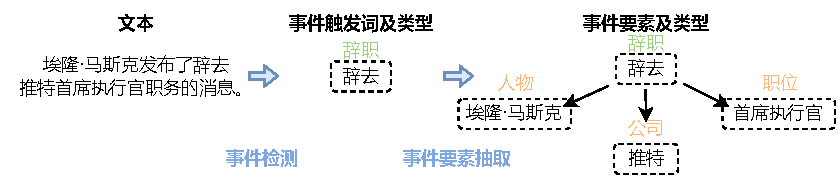
\includegraphics[width=1\linewidth]{figures/chap1/example_chap1.pdf}
   \caption{事件抽取实例}
   \label{example_chap1}
\end{figure}

随着深度学习技术的发展,这两阶段任务均取得相当优异的性能提升。然而,不管是针对事件检测还是事件要素抽取的研究,主要聚焦在特定的模型架构上进行,如循环神经网络、卷积神经网络、图神经网络和预训练语言模型等,忽略了任务中不同模型架构均普遍存在的数据依赖:(1)事件检测数据集中不存在事件的实例比例过高,这种数据不平衡依赖影响了不同模型架构识别事件的能力,从而进一步导致事件检测分类的错误;(2)事件要素抽取数据集中实体提及的类型与要素类型呈现出的强关联依赖,阻碍了不同模型架构更好地建模理解文本中的语义信息。此外,近年来随着各类文本信息资源呈现复杂化的演变趋势,越来越多的事件要素以跨越多个句子的方式出现,其对事件抽取中的事件要素抽取建模方式提出了新要求。因此,研究同时适用于句子级别和文档级别的事件要素抽取方法成为新的研究热点和挑战。然而,(3)现有研究无法在避免共有内在局限性的前提下,实现对不同级别文本中均存在的跨事件依赖关系进行有效构建与利用。

因此,研究事件抽取中的共性数据依赖,可以进一步增强基于不同类型神经网络架构和不同级别文本的现有事件抽取方法的性能表现,提升其作为结构化语义信息应用到不同语言智能化理解领域的质量,支撑事件知识图谱的构建。此外,本研究面向共性数据依赖的特点,赋予其适应新的事件抽取模型架构和建模范式的潜力,具备良好的扩展性。更为重要的是,本研究提出的共性数据依赖是各自所在子领域广泛存在但尚未引起重视的新挑战,具有广阔的深入研究前景。

\section{研究内容与主要贡献}

面对事件抽取系统中不同阶段存在的共性数据依赖,本文从不同的模型架构和文本范围出发,研究通用性的应对方法。其中,针对事件检测阶段普遍存在的数据不平衡依赖问题,提出了基于分类器自适应知识蒸馏的方法;针对事件要素抽取阶段普遍存在的实体类型过度依赖问题,提出了基于多角度对比学习的方法;针对将事件要素抽取扩展到多级别文本时普遍缺乏有效利用跨事件依赖关系的问题,提出了基于分离-融合范式的方法。如图\ref{subtask_relation}所示,上述研究内容覆盖了当前事件抽取系统的关键阶段和应用范围。接下来,具体阐述本文的研究内容和主要贡献如下:

\begin{figure}[htp]
    \centering
   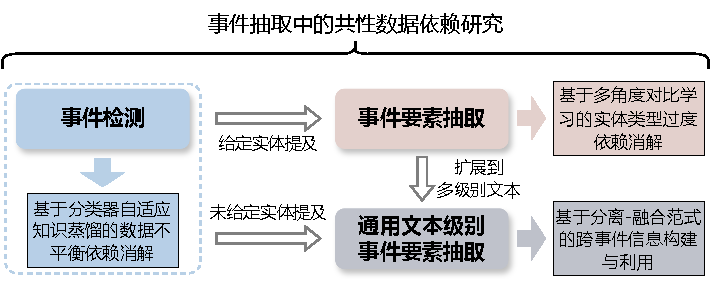
\includegraphics[width=0.8\linewidth]{figures/chap1/subtask-relation.pdf}
   \caption{研究内容关联图}
   \label{subtask_relation}
\end{figure}

\textbf{(1)基于分类器自适应知识蒸馏的数据不平衡依赖消解}

\textbf{问题阐述:}当前事件检测数据集存在严重的数据不平衡,限制了已有不同事件检测模型系统识别事件的能力,进一步降低了模型整体检测性能。针对该问题,相关研究特定于具体的模型架构和任务设计,依赖超参数以适应动态变化的数据不平衡程度,阻碍了可扩展性。

\textbf{研究内容:}针对上述问题,本文工作首先定义和引入句子级别识别信息,并验证该信息在消解数据不平衡依赖导致的性能下降方面的优势。基于此,研究利用知识蒸馏原理自动捕捉句子级别识别信息,提出在事件识别增强网络输入中增加对于句子级别识别信息的构建,并通过分类器参数引导事件检测网络从原始文本中自动学习该信息,实现事件检测性能的增强。

\textbf{主要贡献:}该研究为消解事件检测中存在的数据不平衡依赖问题提供了新颖的角度。与现有的消解方法基于具体数据不平衡程度\textbf{被动}地增强正样本或减弱负样本的训练权重不同,本文工作从数据不平衡依赖影响事件检测性能的方式出发,以此引入了句子级别识别信息进行\textbf{主动}地消解数据不平衡依赖导致的性能损失,并针对性地设计了知识蒸馏框架自动学习该信息。因此,这种主动方式实现了不依赖超参数而自主适应不同模型架构和数据不平衡程度的多维度通用数据不平衡依赖消解。

\textbf{(2)基于多角度对比学习的实体类型过度依赖消解}

\textbf{问题阐述:}不同的事件要素抽取模型在建模事件触发词与实体提及的复杂交互时,受益于实体提及类型信息,忽略了其与要素类型间的强关联性。该强关联性使得不同的事件要素抽取模型在建模中对于实体类型过度依赖,影响了事件要素类型的正确预测。

\textbf{研究内容:}针对上述问题,本文工作首先定义实体类型过度依赖问题并通过实验研究该问题在不同事件要素抽取架构中的存在性。基于此,研究利用监督对比学习分别从正样本和负样本两个角度进行实体类型过度依赖消解,并构建循环训练策略,以实现不同角度消解的高效协作。

\textbf{主要贡献:}该研究提供了在事件要素抽取中利用实体类型信息的新思路。与现有方法关注实体类型信息的\textbf{正面增益}不同,本文工作从实体类型与要素类型的数据特点出发,清晰地定义了实体类型过度依赖,并验证了其在不同模型架构中存在的普遍性,评估了其对于要素类型预测性能产生的\textbf{负面影响}。为了消解该问题,本文工作提出了两种新的监督对比学习方法,聚焦从不同角度减少实例特征表示对于实体类型的依赖性,提升整体文本语义信息的建模质量,通用有效地消解了实体类型过度依赖导致的性能损失。

\textbf{(3)基于分离-融合范式的跨事件信息构建与利用}

\textbf{问题阐述:}当前适用于不同文本级别的事件要素抽取方法存在各自的局限性,而基于多词元链接的建模方法能够有效避免这些局限性并表现出良好的性能潜力。然而,在现有的多词元链接方法中,单一事件建模方式缺乏利用跨事件依赖关系,多事件建模方式需要增加编码序列和链接操作,导致了更多预测错误的积累。

\textbf{研究内容:}针对上述问题,研究结合不同多词元链接建模方式的各自优势,提出分离-融合抽取范式,将跨事件信息获取和事件要素抽取的建模过程进行分离,再将获取的跨事件信息融合到目标事件的要素预测中。遵循该研究范式,进一步提出相应的多词元链接模型,通过设计不同的多词元链接构建和两阶段融合机制,以实现建模不同事件间关联依赖性的同时,保持了高效直接的要素链接推理。

\textbf{主要贡献:}该研究为利用多词元链接进行通用文本级别事件要素抽取构建了新范式。与现有事件建模方式存在\textbf{各自优势}不同,本文工作提出的分离-融合抽取范式,构建了跨事件信息获取和事件要素抽取过程的分离再融合,从而实现了现有不同事件建模方式优势的\textbf{高效统一}。在该范式的指导下,提出了新的多词元链接模型,有效地构建与利用了不同文本级别事件要素抽取共有的跨事件依赖信息。

\section{论文组织结构}

本文工作面向事件抽取系统存在的共性数据依赖,根据\textbf{规划研究目标$\Rightarrow$明确研究内容$\Rightarrow$介绍现有工作$\Rightarrow$分析共性问题$\Rightarrow$阐述技术路线$\Rightarrow$总结研究成果}的行文结构,阐明相应的研究解决方法。如图\ref{organization}所示,将全文划分为六个章节,具体组织安排如下:

\begin{figure}[]
    \centering
   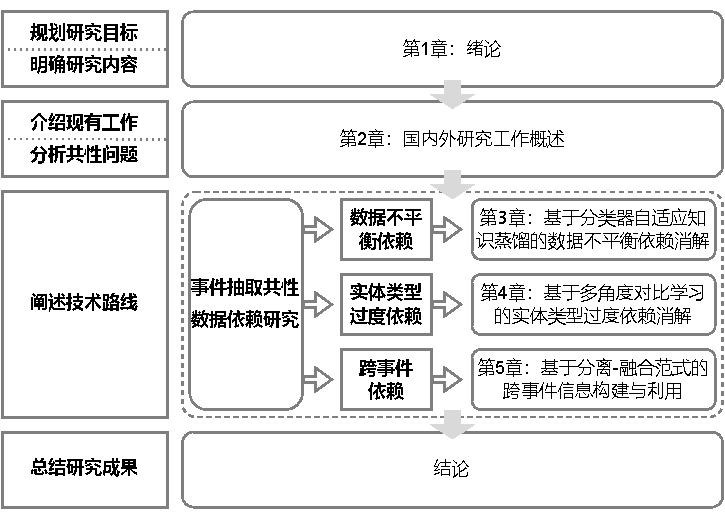
\includegraphics[width=1\linewidth]{figures/chap1/organization.pdf}
   \caption{论文组织结构示意图}
   \label{organization}
\end{figure}

第一章为绪论,介绍了事件抽取任务的研究背景和意义,概述存在于该任务中的共性数据依赖,提炼相应的研究内容和贡献。

第二章为国内外研究工作概述,按照事件抽取系统中的不同阶段分别梳理发展脉络,分析存在的研究问题,归纳研究思路。

第三章围绕事件检测中的数据不平衡依赖消解,研究数据不平衡问题影响整体性能的原因与方式,验证句子级别识别信息在消解其性能损失方面的有效性,进而基于分类器自适应引导的知识蒸馏方法,自动从原始文本中捕捉句子级别信息,实现模型架构通用的数据不平衡自动消解框架。

第四章围绕事件要素抽取中的实体类型过度依赖消解,研究从不同角度消解事件要素抽取建模时对于实体类型信息的过度依赖,通过监督对比学习技术分别从正样本和负样本角度减少实体类型对于实例特征表示的过度影响,并利用循环训练策略优化消解过程,实现文本语义信息建模质量的提升。

第五章围绕通用文本级别事件要素抽取中的跨事件信息构建与利用,研究融合不同多词元链接模型建模事件要素的优势,构建两种多词元链接和两阶段融合机制,以实现跨事件信息获取和事件要素抽取过程的分离再融合,在有效构建事件依赖的同时,保持单事件建模的简单链接预测,提升通用事件要素抽取系统的性能。

最后一章为结论,总结本文研究工作成果,并展望进一步的研究计划。


%%==================================================
%% chapter01.tex for BIT Master Thesis
%% modified by yang yating
%% version: 0.1
%% last update: Dec 25th, 2016
%%==================================================
\chapter{国内外研究工作概述}
\label{chap:recent_work}
本章分别介绍事件检测和两种不同定义下的事件要素抽取技术的发展脉络,并梳理各自存在的共有问题,分析研究思路。

\section{事件检测}
事件检测(Event Detection)是从文本中抽取结构性事件知识的关键步骤~\cite{grishman1997information,ahn2006stages},其旨在识别出具有特定事件类型的事件触发词。事件检测是以事件为中心的信息抽取技术的必要基础,在建模事件要素抽取、事件关系抽取和事件事实性识别等事件知识图谱构建任务时不可或缺,同时也
广泛应用于社交内容分析~\cite{zhou2017event}、知识系统~\cite{li2020gaia,wen2021resin}、故事生成~\cite{li2022event}等多种任务中。

早期的事件检测主要基于模式和特征进行建模。其中,基于模式的方法先构造事件模式,然后在抽取阶段根据事件模式匹配出对应的事件检测信息。事件模式一般基于原始文本或注释信息构建,在早期发展阶段由具备专业语言学知识的专家进行创建。进一步,一些研究利用少量事件模式种子,结合弱监督方法或自助法(Bootstrapping)实现更多事件模式的自动获取~\cite{xu2006automatic,liao2010filtered,kilicoglu2011effective,cao2015improving2}。

而基于特征的方法研究将事件检测分类的线索特征转化为特征向量,并使用机器学习方法进行建模。这些特征可以被划分为局部特征和全局特征。局部特征主要为词法特征和句法特征,包括完整的词、词性标签和依存句法特征等。例如,Chieu等人~\cite{chieu2002maximum}引入一元文法和二元文法等特征信息,并利用最大熵分类器(Maximum Entropy
Classifier)进行事件的检测。Chen等人~\cite{chen2009language}将包括前续字符、现有字符和后续字符的字符级别特征与词级别特征进行结合,并基于最大熵马尔可夫模型(Maximum Entropy Markov Model)检测中文事件触发词。而全局特征则不限于从事件触发词所在句子中得到,其可以为基于跨句子、跨文档和跨事件等获取的实体类型、事件要素信息和词义信息等~\cite{ji2008refining,gupta2009predicting,liao2011acquiring,hong2011using,li2013joint,li2015improving},通常被用于局部信息的补充。例如,Ji等人~\cite{ji2008refining}将相关文档中相同词在不同事件实例中的语义一致性作为全局信息依据,辅助局部的事件预测。Liao等人~\cite{liao2011acquiring}构建无监督主题模型如LDA(Latent Dirichlet Allocation),以获取文档级别的全局信息,用于事件检测任务。Li等人~\cite{li2013joint}在建模中融合了不同事件的依赖关系,如事件触发词间的依赖路径和上下文信息。然而,基于特征的方法通常使用独热向量表示构造的特征,易导致数据稀疏问题。更重要的是,不管基于模版还是特征的方法,都需要具备语言学知识的专业人士进行构建,对于一些低资源语言来说人力成本变得更加昂贵。因此,随着深度学习技术的快速进步,其能够自动从文本中学习语义表示的优势在事件检测任务中得以突显。接下来,本章根据使用的神经网络架构类型进行分别介绍。

\subsection{基于卷积神经网络的方法}

卷积神经网络(Convolutional Neural Networks,CNN)实质为多层感知机的变种形式,受益于其卷积核带来的权重共享和较小感受野,能够以较小的参数规模和计算复杂度实现特征信息的获取。在自然语言处理中,通常将传统二维卷积核的其中一个维度设置为词向量的维度,只改变另一维卷积操作的尺寸大小,将文本中多个词(或字符)组成的片段信息线性映射到特征空间中~\cite{zhang2015sensitivity},实现自动捕捉这些文段的语义和句法信息。具体来说,给定$n$个词组成的句子文本$\left\{w_{1}, w_{2}, \cdots, w_{n}\right\}$,对应的向量输入为$\left\{\boldsymbol{x}_{1}, \boldsymbol{x}_{2}, \cdots, \boldsymbol{x}_{n}\right\}$,假设卷积窗口大小为$k$,则可得任意一个利用该卷积核运算的特征结果:
\begin{equation}
    a_{i}=f\left(\boldsymbol{W} \otimes \boldsymbol{x}_{i: i+k-1}+b\right)
\end{equation}
其中$\boldsymbol{W}$和$b$为待学习训练的参数,$f(\cdot)$为激活函数,$\boldsymbol{x}_{i: i+k-1}$表示从向量$\boldsymbol{x}_{i}$到$\boldsymbol{x}_{i+k-1}$的拼接,$\otimes$为卷积计算。在实际应用中,为了建模特征的多样性,在每个卷积层中采用多个卷积核进行对应特征的捕捉。

在事件检测中,Nguyen和Grishman~\cite{nguyen2015event}为最早应用CNN的研究者。在其构建的方法中,首先将文本中每个词对应的词向量、实体类型向量和相对于目标预测词的位置向量进行串接,然后输入到包含不同尺寸卷积窗口的卷积层中,最后通过最大池化操作得到目标词的特征表示,从而进行最终的事件预测。为了在编码词法特征和句法特征时能够更多地关注到事件触发词信息,Chen等人~\cite{chen2015event}在DMCNN模型中提出了一个动态池化操作去替代传统的最大池化操作,其根据目标预测词的位置将经过卷积层得到的特征表示划分为两部分,分别进行最大池化操作。如图\ref{dmcnn}所示,根据“died”的位置将卷积层得到的向量表示划分为两个部分进行池化处理。与使用卷积层挖掘连续文段信息不同,Nguyen等人~\cite{nguyen2016modeling}设定窗口长度并枚举所有符合该长度要求的非连续文段。然后,使用卷积层建模这些文段,并采用动态规划算法得到其中语义信息最显著的序列,用于最终的事件预测,从而实现非连续词间的长依赖信息的获取。

\begin{figure}[htp]
   \centering
   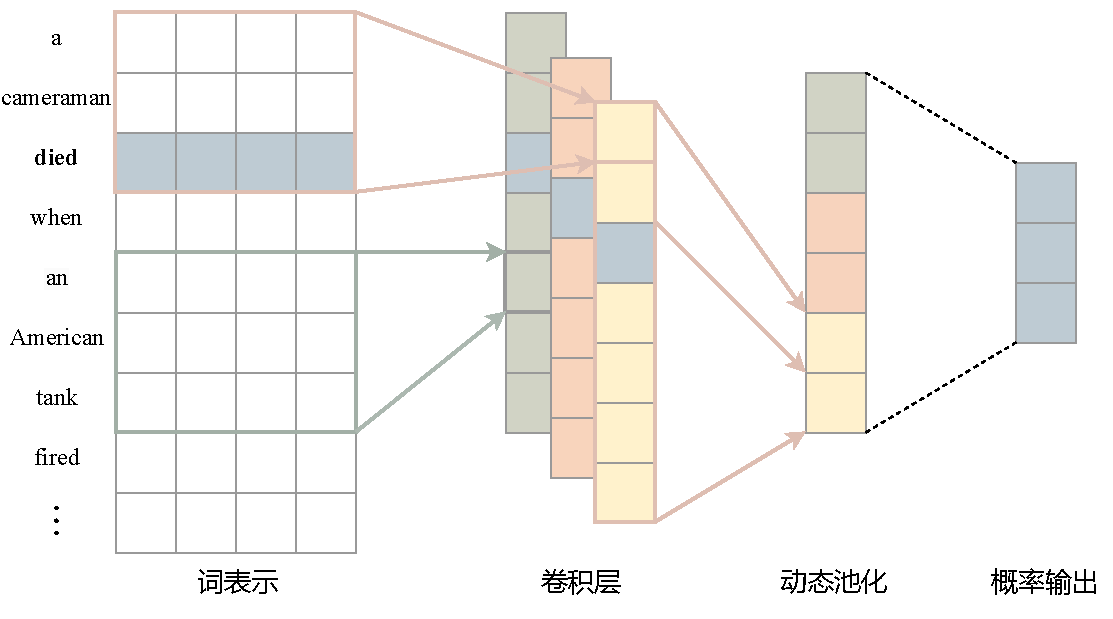
\includegraphics[width=0.8\linewidth]{figures/chap2/dmcnn.pdf}
   \caption{DMCNN模型示意图}
   \label{dmcnn}
\end{figure}

\subsection{基于循环神经网络的方法}

循环神经网络(Recurrent Neural Networks,RNN)\cite{rumelhart1986learning}常用于序列信息的建模,其与传统的全连接网络不同,每层的节点之间存在连接,从而能够更好地捕捉序列中的顺序关联。由于自然语言文本可以视作词组成的序列,RNN可以高效利用到单词顺序对特征编码和结果预测的影响,因而广泛应用在自然语言理解和自然语言生成任务中。具体地,如图\ref{rnn}所示,传统的单步RNN可以看作是相同的计算操作在不同时间步的重复叠加组合,假设$n$个词组成的文本序列向量输入为$\left\{\boldsymbol{x}_{1}, \boldsymbol{x}_{2}, \cdots, \boldsymbol{x}_{n}\right\}$,则第$t$个时间步对应的输出向量$\boldsymbol{y}_{t}$可得:
\begin{equation}
    \begin{aligned}
& \boldsymbol{h}_t=f\left(\boldsymbol{W}^h\left(\boldsymbol{h}_{t-1} ; \boldsymbol{x}_t\right)+\boldsymbol{b}^h\right) \\
& \boldsymbol{y}_t=g\left(\boldsymbol{W}^y \boldsymbol{h}_t+\boldsymbol{b}^y\right)
\end{aligned}
\end{equation}
其中$f(\cdot)$和$g(\cdot)$通常为非线性激活函数,$\boldsymbol{h}_t$为当前时间步的隐藏层状态向量,$\boldsymbol{W}^h$、$\boldsymbol{W}^y$、$\boldsymbol{b}^h$和$\boldsymbol{b}^y$为不同时间步共享的训练参数。进一步,以LSTM~\cite{hochreiter1997long}和GRU~\cite{cho2014learning}为代表的RNN变体被提出,以缓解传统RNN建模长序列时产生的梯度消失和梯度爆炸现象。

\begin{figure}[htp]
   \centering
   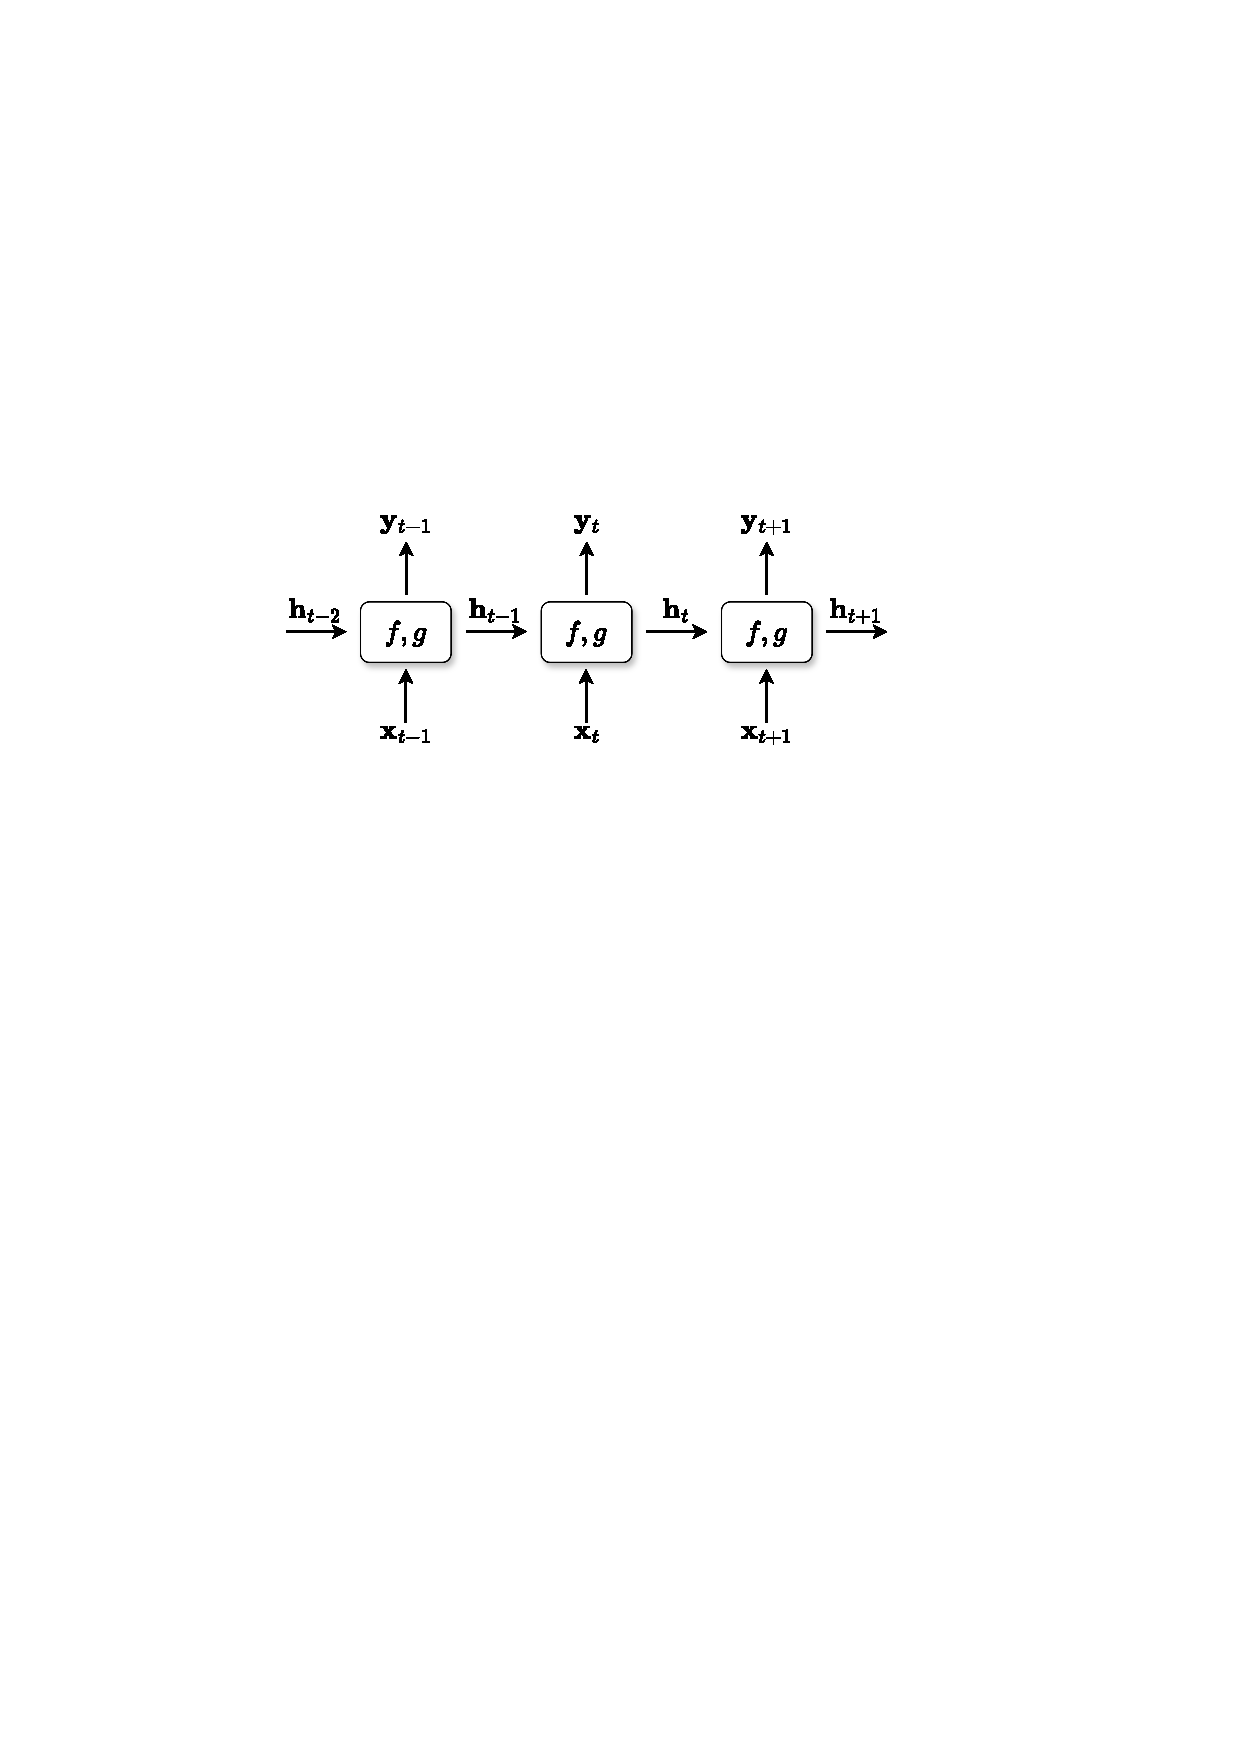
\includegraphics[width=0.7\linewidth]{figures/chap2/rnn.pdf}
   \caption{RNN示意图}
   \label{rnn}
\end{figure}

在事件检测任务中,Ghaeini等人~\cite{ghaeini2016event}最先应用了LSTM,其根据候选触发词将文本划分为左侧上下文、候选触发词本身和右侧上下文,分别使用LSTM进行编码并进行特征表示的串接,以用于最终的多分类事件预测。Jagannatha等人~\cite{jagannatha2016bidirectional}则将医疗领域的事件检测转化为序列标注问题,结合预定义事件类型和BIO(Begin,Inside,Outside)标注策略,使用双向LSTM或GRU进行建模。Orr等人~\cite{orr2018event}将依存句法信息转化为有向非循环图,并基于GRU提出了一个新的变种模型,以更好地在事件检测中利用句法信息和上下文信息。为了解决GRU和LSTM等网络中门控计算依赖之前时间步的信息而导致的无法并行计算的问题,Zhang等人~\cite{zhang2019empower}基于简单循环单元(Simple Recurrent Unit,SRU),构建两个SRU模型分别用于获取事件检测中单词级别和字符级别的语义特征,以实现性能和计算效率的更好平衡。

虽然RNN相比于CNN能够建模更长的词间依赖关系,但其建模的有效上下文长度仍然受限,为了进一步提高上下文信息的利用效率,一些研究者在此基础上引入了注意力机制。例如,Chen等人~\cite{chen2018collective}利用跨句信息和不同事件间的相关性增益事件检测的性能。在该模型中,其一方面基于双向LSTM网络在句子级别得到每个词的特征表示,然后使用两层注意力机制获取对应的文档级别特征表示,并构建门控机制实现不同级别信息的融合。另一方面,其构建了多层LSTM的变体网络层TLSTM,其在LSTM门控计算中增加了通过注意力机制得到的前一层预测的所有词的事件类型标签信息,从而隐式地构建不同事件预测结果的关联性。Lou等人~\cite{lou2021mlbinet}同样基于LSTM网络和注意力机制构建一个编码器-解码器架构,以利用跨句范围内的语义信息和事件间的依赖关系。在编码器中,使用双向LSTM网络进行编码,并基于自注意机制融合长距离上下文语义信息。在解码器中,分别使用融合了前一个词标签预测信息的双向RNN解码器,并串接相应的解码表示,以获取能够双向捕捉同一句子内不同事件关联依赖的事件标签向量。进一步考虑到跨句范围的事件依赖关系,其引入了另一个LSTM网络编码已得到的事件标签向量,从而聚合跨句范围内不同句子的整体事件信息。最后,为了能够在解码中利用到聚合的事件信息,作者们再次叠加新的双向解码层并融合前后相邻句子的事件信息。通过重复该融合过程,更远距离的句子事件信息得以被捕获,从而增益目标事件的检测。Liu等人~\cite{liu2019event}探索不依赖事件触发词标注信息去预测文本中存在的事件。作者们将该预测过程建模为多标签问题,使用LSTM编码得到词的特征表示,并使用不同的预定义事件类型向量作为查询向量,得到相应的文本整体表示,以预测对应事件类型的存在。

此外,一些研究针对CNN和RNN的特点,探索融合各自的优势进行事件检测任务的建模。例如,Feng等人~\cite{feng2018language}提出了一个融合CNN和RNN的混合神经网络,以用于多语言场景下的事件检测任务。其在使用双向LSTM网络建模上下文序列信息的同时,利用CNN获取局部文本特征表示。然后,串接这两种建模网络得到的信息,以进行多种语言数据集中的触发词检测。Lu等人~\cite{lu2019distilling}认为现有事件检测模型具备良好地区分不同上下文中容易混淆的高频触发词的能力,但缺乏识别罕见或未出现的触发词的泛化知识。为此,其一方面结合了RNN和注意力机制,建模以候选触发词为中心的上下文表示,以提供事件检测的触发词区分能力,并构建额外的二分类辅助任务增强候选触发词对其上下文表示的影响。另一方面,使用DMCNN~\cite{chen2015event}建模与候选触发词无关的上下文表示,以提供事件检测的触发词泛化能力。并且,利用生成对抗技术~\cite{creswell2018generative}降低候选触发词对其上下文表示的影响。最后,基于门控机制实现不同上下文表示的高效融合,以增强事件检测的整体性能。

\subsection{基于图神经网络的方法}

句法表示能够提供单词与其句法相关上下文的直接连接,但无论CNN还是RNN,均主要聚焦于建模自然语言文本中的序列。因此,为了更加高效直接地利用这类句法信息,近年来基于图进行建模的图神经网络(Graph Neural Networks,GNN)在自然语言处理的各个领域均得到广泛应用。在事件检测任务中,主要使用的是GNN中的图卷积神经网络(Graph Convolutional Neural Networks,GCN)\cite{kipf2016semi}。给定图$\mathcal{G}=(\mathcal{V}, \mathcal{E})$,其中$\mathcal{V}$为图中节点的集合,$\mathcal{E}$为图中边的集合。假设第$l$层图卷积的特征表示$\boldsymbol{H}^l=\left\{\boldsymbol{h}_i^l\right\}$,则第$l+1$层图卷积的特征表示可计算如下:
\begin{equation}
    \boldsymbol{h}_i^{l+1}=f(\sum_{(i, j) \in \mathcal{E}} \alpha_{i j}^l \boldsymbol{W}^l \boldsymbol{h}_j^l+\boldsymbol{b}^l)
\end{equation}
其中$\boldsymbol{W}^l$和$\boldsymbol{b}^l$为待学习训练的参数,$f(\cdot)$为非线性激活函数,$\alpha_{i j}^l$为节点$i$指向节点$j$的边对应的权重值。图\ref{gcn}展示了由四个节点组成的一个GCN示例。

\begin{figure}[htp]
   \centering
   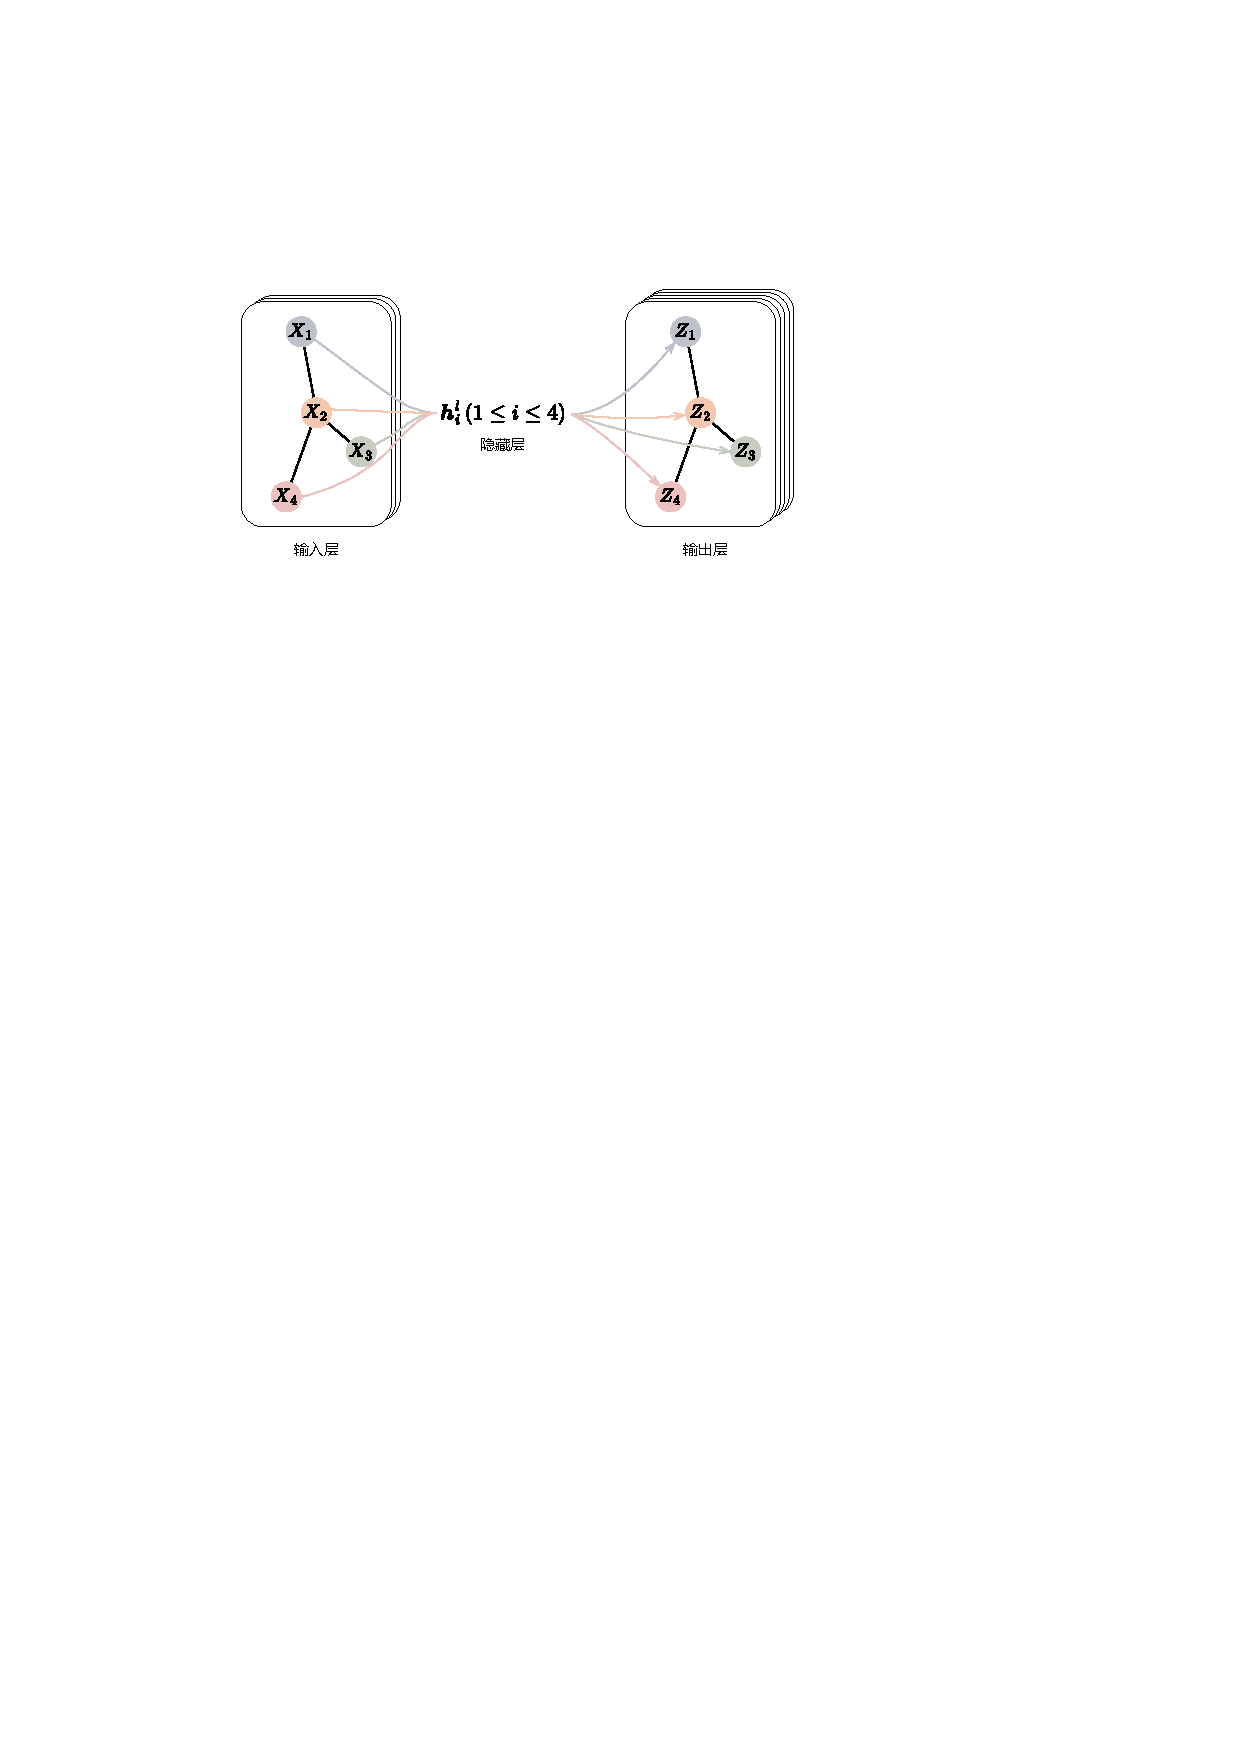
\includegraphics[width=0.7\linewidth]{figures/chap2/gcn.pdf}
   \caption{GCN示意图}
   \label{gcn}
\end{figure}

Liu等人~\cite{liu2018jointly}和Nguyen等人~\cite{nguyen2018graph}为最早在事件检测任务中使用GCN的研究者。在其研究工作中,首先使用自然语言处理工具将文本解析成结构化的依存句法树,然后设计策略将得到的依存句法树转化成可以用于建模GCN的图。具体地,图中的节点为句子中所有的单词,而节点间的边可以区分为三类。第一类边为直接从依存句法树中得到的正向边。假设在该树结构中,从单词$w_{i}$到单词$w_{j}$存在任意类型的依存句法关系,则在图中构建由节点$i$指向节点$j$的有向边。第二类边为所有第一类边的逆向边,以保证图中信息的逆向传播。第三类边则为每个节点指向自身的闭环边,使得构建的图能够形成闭环。基于所构建的图,进行多层GCN的迭代,实现依存句法树中多跳依存信息的高效获取。首先,利用双向LSTM网络层进行编码,以捕捉序列上下文信息。进一步,将编码得到的特征表示输入到GCN中,以获取构建的图中的结构化信息,其中不同类型的边使用不同的学习训练参数$\boldsymbol{W}^l$和$\boldsymbol{b}^l$,权重值$\alpha_{i j}^l$计算如下:
\begin{equation}
    \alpha_{i j}^l=\sigma(\boldsymbol{h}_j^l \boldsymbol{V}^l+d^l)
\end{equation}
其中$\boldsymbol{V}^l$和$d^l$为权重计算时学习的参数,且同一种类型的边计算时进行参数共享。$\sigma(\cdot)$为sigmoid激活函数。为了进一步在GCN中减少与候选触发词无关的信息干扰,Lai等人~\cite{lai2020event}基于候选触发词的特征表示生成对应的门控向量,从而实现对其他单词特征表示的过滤筛选:
\begin{equation}
    \boldsymbol{g}^l=\sigma\left(\boldsymbol{W}_g^l \boldsymbol{e}_t\right)
\end{equation}
\begin{equation}
    \boldsymbol{m}_i^l=\boldsymbol{g}^l \odot \boldsymbol{h}_i^l
\end{equation}
其中$\boldsymbol{W}_g^l$为学习的参数,$\boldsymbol{e}_t$为候选触发词在输入GCN前的编码表示,$\odot$为元素依次相乘操作。基于该门控方法获取的不同单词特征表示,最终用于辅助候选触发词的事件预测。此外,由于图网络中不同层建模上下文语义信息的侧重点有所不同,因此需要保证门控向量的多样性。为此,其设计了额外的正则化损失减少相同门控向量筛选过滤同一单词不同层特征表示后的相似程度。同时,作者们利用依存句法树中的依赖路径距离指导模型更好地感知不同单词对于候选触发词的重要程度。

此外,由于在事件检测常用的ACE2005数据集中,超过一半的事件触发词在其对应的依存句法树中和关联实体或者单词没有直接的连接。为此,Liu等人~\cite{liu2018jointly}和Nguyen等人~\cite{nguyen2018graph}通过叠加多层GCN进行建模。然而,随着GCN层数的叠加,图中节点的特征表示将会变得愈加相似,导致过平滑问题~\cite{zhou2020graph}。为了解决该问题,Yan等人~\cite{yan2019event}直接构建包含多跳依存句法关系的图,以替代在基于单跳依存句法关系构建的图上叠加多层GCN。与Liu等人~\cite{liu2018jointly}和Nguyen等人~\cite{nguyen2018graph}使用相同的策略,其首先将解析得到的依存句法树转化成包含正向边、逆向边和闭环边三种类型的有向图。不同的是,Yan等人~\cite{yan2019event}进一步根据各个类型得到对应的邻接矩阵,并计算任意$k$跳依存句法关系图的邻接矩阵如下:
\begin{equation}
    \boldsymbol{A}_{ type}^k=\left(\boldsymbol{A}_{type}\right)^k
\end{equation}
其中$\boldsymbol{A}_{type}$可为正向边、逆向边和闭环边分别对应的邻接矩阵。基于$\boldsymbol{A}_{ type}^k$,为了捕捉到依存句法树中单词间$k$跳的句法关系,其使用单层图注意力网络(Graph Attention Network,GAT)\cite{velivckovic2017graph}替代多层GCN进行编码如下:
\begin{equation}
    \boldsymbol{h}_i=f( \sum_{j=1}^n\left(u_{i j} a_{i j}\left(\boldsymbol{W}_{a} \boldsymbol{p}_j+\boldsymbol{\epsilon}\right)\right))
\end{equation}
\begin{equation}
    u_{i j}=\frac{\exp \left(e_{i j}\right)}{\sum_{j \in \mathcal{N}_i} \exp \left(e_{i j}\right)}
\end{equation}
其中$e_{i j}=g\left(\boldsymbol{W}_1\left[\boldsymbol{W}_2 \boldsymbol{p}_i;\boldsymbol{W}_2 \boldsymbol{p}_j\right]\right)$,$\boldsymbol{W}_1$、$\boldsymbol{W}_2$、$\boldsymbol{W}_{a}$和$\boldsymbol{\epsilon}$为待学习训练的参数,$a_{i j}$表示$\boldsymbol{A}_{ type}^k$对应的图中节点$i$指向节点$j$的边对应的权重值,$\boldsymbol{p}_j$为图中节点$j$的输入向量,$\mathcal{N}_i$表示在$\boldsymbol{A}_{ type}^k$对应的图中节点$i$的邻接节点集合,$f(\cdot)$和$g(\cdot)$分别表示ELU和LeakyReLU激活函数。最后,利用注意力机制聚合每个单词在不同跳句法关系图上建模获取的特征表示,以用于最终的事件类型预测。

与上述研究工作不同,最近的方法考虑进一步利用依存句法关系的类型信息。Cui等人~\cite{cui2020edge}提出了在GCN中构造一个邻接张量,以利用其中的向量表示图中任意两个节点的关系。若图中节点间的依存句法关系类型相同,则对应的向量初始化也相同。基于此,分别设计了图中节点表示和边表示的相互迭代更新方法,以实现高效建模邻接张量中的异质信息。Liu等人~\cite{liu2021self}在Cui等人~\cite{cui2020edge}研究工作的基础上,考虑了依存句法树中句法关系存在方向性的区别,初始化了两个非对称的邻接张量。然而,静态的邻接张量仍无法有效建模依存句法信息之外不同节点间潜在的依赖关联,为此其进一步构建了一个自注意力模块,以动态更新自注意力张量,并融入到节点表示和边表示的迭代计算中。

此外,Mi等人~\cite{mi2022event}利用依存句法树和语义角色标注构造双重关系图,在考虑句法结构的同时,引入互补的语义关系信息,以减少句法信息带来的噪音和冗余。具体地,在构建双重关系图时,保留在依存句法树中与候选触发词直接连接的单词和句法关系,将其他句法关系替换成表示与候选触发词的连接距离的虚拟关系。同时,根据语义角色标注结果引入语义关系的连接。基于构建的关系图,构建关系增强的GAT,其基于对应关系向量和上下文信息进行注意力机制的权重计算。

\subsection{基于预训练语言模型的方法}
近年来,预先基于大规模无标签文本数据进行训练,再根据具体下游任务微调的建模方式广泛应用在各种自然语言处理任务中。在事件检测任务中,通常使用以BERT (Bidirectional Encoder Representations from Transformers)\cite{kenton2019bert}为代表的双向语言模型作为进一步微调使用的预训练语言模型。BERT主要由多层Transformer~\cite{vaswani2017attention}编码器组成,其每一层的架构如图\ref{transformer}所示。该架构由$N$(一般设置为6)个相同的子网络层组成,每个子网络层主要包括多头注意力和前馈神经网络,并辅以加和连接和层归一化操作。在多头注意力(MultiHead)中,并行学习$h$组不同的线性变换层参数分别将自注意力计算输入中的键矩阵$\boldsymbol{K}$、值矩阵$\boldsymbol{V}$和查询矩阵$\boldsymbol{Q}$映射到各自的特征空间中,然后拼接对应的自注意力计算结果,其中的$h$即为多头的数量,具体可表示如下:
\begin{equation}
    \begin{aligned}
\textrm{MultiHead}(\boldsymbol{Q}, \boldsymbol{K}, \boldsymbol{V}) & = \left[head_1; \cdots; head_{h}\right] \boldsymbol{W}^O \\
{head}_{i} & =\textrm{Attention}\left(\boldsymbol{Q} \boldsymbol{W}_i^Q, \boldsymbol{K} \boldsymbol{W}_i^K, \boldsymbol{V} \boldsymbol{W}_i^V\right)
\end{aligned}
\end{equation}
其中$\boldsymbol{W}_i^Q$,$\boldsymbol{W}_i^K$,$\boldsymbol{W}_i^V$和$\boldsymbol{W}^O$为学习训练的参数,
$\textrm{Attention}$为缩放点积注意力,计算如下:
\begin{equation}
    \textrm{Attention}(\boldsymbol{Q}, \boldsymbol{K}, \boldsymbol{V})=\textrm{softmax}\left(\frac{\boldsymbol{Q} \boldsymbol{K}^T}{\sqrt{d_k}}\right) \boldsymbol{V}
\end{equation}
其中$d_k$为键矩阵$\boldsymbol{K}$和查询矩阵$\boldsymbol{Q}$中的向量维度。

\begin{figure}[htp]
   \centering
   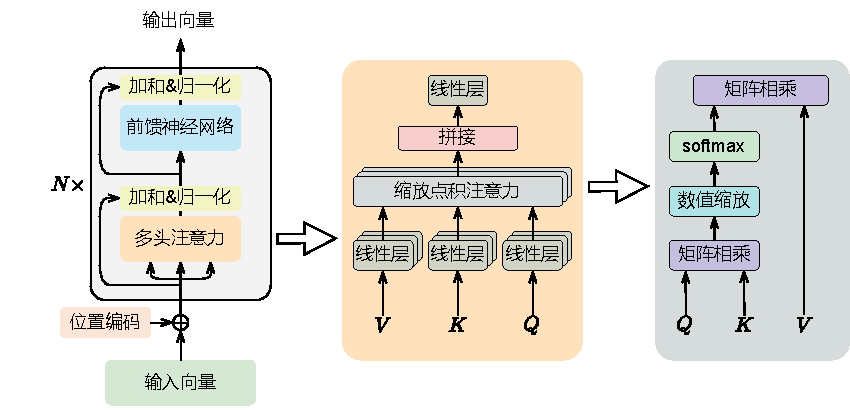
\includegraphics[width=1\linewidth]{figures/chap2/transformer.pdf}
   \caption{Transformer编码器示意图}
   \label{transformer}
\end{figure}

在预训练阶段,BERT利用文档级别的大规模英文文本语料集,其包括英文维基百科数据和BooksCropus语料库,执行如下两个预训练任务:

(1)遮掩语言模型(Masked Language Model,MLM):受完形填空的启发,该任务随机选取15\%已切分的WordPiece~\cite{wu2016google}输入序列中的词元进行遮掩,并使用BERT预测被遮掩的词元。但该遮掩训练方式与微调阶段存在不一致。因此,基于此15\%被选中的词元作进一步操作:保留其中80\%词元的遮掩操作,取消其中10\%词元的遮掩操作,并将剩下的词元随机替换成其他词元。通过提供预测词元的不确定性,促使模型更多地学习到全局上下文信息。

(2)下一句预测(Next Sentence Prediction,NSP):以文本对方式构建该任务输入,表示为“$[CLS]+S_{A}+[SEP]+S_{B}+[SEP]$”,其中$[CLS]$和$[SEP]$为特殊词元。该任务仅保留语料数据中一半句子的真实下一句作为$S_{B}$,另一半句子的$S_{B}$从语料集中随机选取得到,其旨在通过特殊词元$[CLS]$预测$S_{B}$是否被随机替换。通过此任务的训练,提升BERT模型在自然语言推理和问答等任务上的语言理解能力。

在下游任务微调阶段,根据任务的特点,选择单个文本或文本对输入到预训练BERT模型中,并叠加额外的设计模块进行训练损失微调。在事件检测任务中,Yang等人~\cite{yang2019exploring}首先利用BERT模型获取各个词的特征表示并构建多分类器进行事件类型的建模。Wang等人~\cite{wang2019adversarial}将DMCNN~\cite{chen2015event}模型中的CNN替换成BERT,保留其动态池化操作,构建对应的DMBERT进行事件预测。Liu~\cite{liu2020event}等人将事件检测问题转化为机器阅读理解任务,其简单地构建了一个特殊查询命令“[EVENT]”并和待抽取文本进行串接输入到BERT中,对于每个单词使用多分类的方法建模其对应的事件类型信息。类似地,Du等人~\cite{du2020event}设计了四类静态的问答模版用于事件检测,包括“what is the trigger”、“trigger”、“action”和“verb”,并同样使用多分类器进行事件类型的建模预测。与Liu等人~\cite{liu2020event}和Du等人~\cite{du2020event}不同,一些研究考虑显示地在预训练语言模型中利用事件类型的语义知识,深度建模其与待抽取上下文间的交互关系。例如,Li等人~\cite{li2020event}为了在BERT中利用到不同事件类型名称本身的语义信息,其将事件检测任务转化为多轮问答。具体地,首先设计固定的问题模版预测事件触发词的开始和结束位置,然后枚举所有的预定义事件类型并和已预测的触发词文本、触发词位置进行串接,根据特殊字符$[CLS]$进一步确定所属的事件类型。该方法不依赖预定义的事件类型数目,可扩展到新的事件类型预测,在零样本和少样本场景下同样表现出良好的性能潜力。Wang等人~\cite{wang2022query}使用事件类型名称和高频原型触发词作为对应事件类型的描述,然后枚举所有的事件类型描述并分别与待抽取文本串接,利用二分类方式建模对应的事件触发词。进一步,在相同的框架下,Wang等人~\cite{wang2022art}丰富了事件类型的描述模版,增加了事件定义、相关的事件要素类型、自动学习的软模版和人工构建的事件模版等信息。

进一步,一些工作基于BERT深入研究事件检测模型的鲁棒性、知识增强和预测模式等问题,以更好地挖掘预训练语言模型的潜力。例如,现有事件检测建模过于依赖词法信息,欠缺良好的上下文建模能力,从而导致在预测罕见或未出现的触发词时性能下降明显~\cite{lu2019distilling}。针对该问题,Liu等人~\cite{liu2020does}提出了两种上下文遮掩策略,以提升BERT模型在事件检测任务上的鲁棒性。第一种为句内策略,旨在提升模型学习句内上下文中的显著语义信息。具体地,固定已训练的事件检测模型的参数,其首先只遮掩候选触发词并使用遮掩向量作为查询向量计算对应的上下文注意力分布$\boldsymbol{\alpha}_{u}$,然后随机采样多种遮掩序列同样计算其上下文注意力分布。如果其中存在遮掩序列能够提升模型的预测结果,则以对应的上下文注意力分布作为训练目标,减少其与$\boldsymbol{\alpha}_{u}$的方差。第二种为句间策略,其基于单词分布假设~\cite{harris1970distributional},增加相同事件类型的触发词被遮掩后的上下文间的相似度,反之则减少对应的上下文间的相似度。类似地,Tong等人~\cite{tong2020improving}也观察到现有方法在预测罕见和未出现的事件触发词时性能表现不佳,并将其归因于数据集中存在的事件类型长尾分布。为了解决该问题,其基于知识蒸馏技术,将根据词义获取的开放域触发词知识用于提升对这两类事件触发词的识别。具体地,首先使用WordNet~\cite{miller1990introduction}数据库从词义的角度实现对New York Times~\cite{sandhaus2008new}语料库的快速大规模标注,以获取开放域触发词知识。然后,构建知识蒸馏框架,促使教师网络和学生网络在监督数据集和大规模标注数据集上的预测概率均保持相似,从而实现开放域触发词知识的迁移。其中,在教师网络输入文本中使用两个特殊字符标注触发词的边界信息,而在学生网络输入文本中则遮掩对应的触发词,从而促使基于上下文信息的学生网络从教师网络中更好地学习识别触发词的能力。Liu等人~\cite{liu2022saliency}使用基于BERT训练的事件检测模型量化区分事件类型的潜在模式并根据模式的不同采取相应策略增强预测性能。具体地,利用可解释领域的积分梯度算法(Integrated Gradient)\cite{sundararajan2017axiomatic},计算文本中每个单词$w_{i}$对于事件预测的贡献值,具体如下:
\begin{equation}
\boldsymbol{\alpha}_{w_i}=\left(\boldsymbol{x}_i-\boldsymbol{x}_i^{\prime}\right) \times \int_{\alpha=0}^1 \frac{\partial \mathcal{L}\left(t ; \boldsymbol{X}^{\prime}+\alpha \times\left(\boldsymbol{X}_s-\boldsymbol{X}^{\prime}\right)\right)}{\partial \boldsymbol{x}_i} d \alpha
\end{equation}
其中$\boldsymbol{x}_i$为$w_{i}$由BERT编码得到的特征表示,$\boldsymbol{X}_s$为文本中所有单词对应的特征表示组成的序列,
$\boldsymbol{X}^{\prime}$为对应于$\boldsymbol{X}_s$的零向量序列,$\boldsymbol{x}_i^{\prime}$为$\boldsymbol{X}^{\prime}$序列中第$i$个向量,$t$为预测的事件类型的独热向量表示。

基于此,进一步归一化得到的预测贡献值,
% \begin{equation}
% \alpha_{w_i}=e^{\left\|\boldsymbol{\alpha}_{w_i}\right\|_2} / \sum_{n=1}^N e^{\left\|\boldsymbol{\alpha}_{w_n}\right\|_2}
% \end{equation}
% 其中$\|\|$为$L_{2}$范数。
并根据每个单词的贡献值,计算不同事件类型的触发词在整体训练集中的平均贡献。然后,设置阈值且根据每个事件类型触发词的平均贡献将其划分为触发词依赖的事件或上下文依赖的事件。对于前者,构建基于BERT的事件检测模型并在输入中使用额外的单词显著贡献向量来标记各个单词的贡献值信息,辅助模型聚焦于具备高贡献值的单词进行建模。对于后者,构建另一个基于BERT的事件检测模型并在输入中串接具有高贡献值的上下文片段,辅助模型更好地利用相关上下文信息。在测试阶段,集成此两个事件检测模型的预测,得到最终的检测结果。
% 针对BERT由于输入长度的限制而无法在事件检测中编码更多的跨句信息,Veyseh等人~\cite{veyseh2021modeling}基于强化学习算法REINFORCE自动学习从跨句信息中选择重要的上下文信息参与到BERT编码中。具体地,枚举选择不同句子组成的上下文,考虑从BERT建模事件检测的性能、选择上下文与目标句子的语义相似性和实体共指的数量等多个角度评估对应的奖励值,从而指导算法参数的更新。

此外,存在一些研究工作基于自回归预训练语言模型进行事件检测的数据增广。例如,Veyseh等人~\cite{veyseh2021unleash}使用GPT-2~\cite{radford2019language}生成训练数据。为了降低生成数据中的噪音信息,其设计了教师-学生网络。教师网络使用高质量数据集进行训练得到,而学生网络则同时使用高质量数据和生成数据进行训练,并保持与教师网络的知识一致性。

近年来,以ChatGPT、PaLM~\cite{chowdhery2023palm}和LLaMA~\cite{touvron2023llama}为代表的大语言模型(Large Language Models,LLMs)在自然语言处理的很多研究领域取得了令人印象深刻的性能表现。在事件检测任务上,一些研究者基于ChatGPT进行了相关性能的评估。例如,Li等人~\cite{li2023evaluating}基于零样本场景评测了ChatGPT在事件检测任务上的性能。具体地,其设计的输入提示模版包括对于任务的描述、预定义的事件类型集合、待抽取的文本内容和形式化的输出格式要求。Gao等人~\cite{gao2023exploring}丰富了输入提示模版的内容,一方面其扩充了对于各个预定义事件类型的详细描述,同时给出了正确样例和错误样例的输入输出信息。基于此,选取测试集中部分样例进行了性能评测。进一步,Han等人~\cite{han2023information}设计了与Li等人~\cite{li2023evaluating}相似的提示模版,并引入情景学习(In-Context Learning,ICL)\cite{brown2020language}和思维链(Chain-Of-Thought,COT)\cite{wei2022chain}技术,提升了少样本场景下ChatGPT在事件检测任务上的性能。具体地,在原有提示模版的基础上,添加5个从训练集中随机采样的训练数据的文本信息和对应的正确事件检测结果作为示例,从而构建出5-shot ICL提示模版。对于5-shot COT提示模版,其关于事件检测的解释过程由人工进行构造。虽然这些研究采取了提供负样例、ICL和COT等不同策略提升性能,但评估结果均表明ChatGPT在事件检测任务上的性能仍与现有监督模型存在明显差距。

\section{给定实体提及的事件要素抽取}
\label{section2_2}
事件要素抽取(Event Argument Extraction)旨在根据事件检测得到的事件触发词和事件类型信息,进一步识别事件中存在的事件要素以及对应的事件要素类型。识别得到的事件要素作为结构化的语义信息,广泛应用于多种下游任务~\cite{wen2021resin,wu2022cross,fung2023deepmaven,liu2023covid}。

现有的事件要素抽取任务存在两种不同的定义方式。第一种定义方式主要基于自动内容提取项目(Automatic Content Extraction,ACE)\footnote{http://projects.ldc.upenn.edu/ace/}。该项目在评估设置中将实体提及的识别和事件要素抽取分离,因此在事件要素抽取中可以直接利用到实体提及的标签信息。具体地,给定待抽取文本、事件触发词和事件类型,本定义下的事件要素抽取将文本中已知存在的实体提及均视作候选事件要素,旨在识别出所有作为事件要素出现的实体提及,并给出对应的预定义事件要素类型。由于ACE项目聚焦于句子级别的信息标注,待抽取文本一般为单个句子。随着近年来文本信息朝着复杂化方向演变,出现了以RAMS~\cite{ebner2020multi}和WikiEvents~\cite{li2021document}为代表的文档级别事件要素抽取数据集,其将实体提及的识别包含在事件要素抽取任务中。为了更好地研究适合不同文本级别的事件要素抽取模型,最近的一些事件要素抽取方法~\cite{ma2022prompt}给出了不同的定义方式。具体地,给定由单个句子或多个句子组成的待抽取文本、事件触发词和事件类型,该定义下的事件要素抽取旨在识别出每个事件要素的文段范围以及对应的预定义事件要素类型。与第一种定义不同的是,其要素类型的预测范围特定于给定事件类型,而非数据集中所有预定义的要素类型。

基于定义方式的不同,相应事件要素抽取研究工作的建模方式也存在较大差异。因此,本章主要介绍基于第一种定义方式的技术发展情况,其相关工作均根据ACE项目或类似的定义进行建模和评估。而第二种定义方式下的事件要素抽取技术将在下一章节进行梳理。

与事件检测任务相似,早期的事件要素抽取方法同样基于人工设计的事件模式或特征进行构建。其中,基于事件模式的方法结合词性标注结果和候选事件模式,匹配出对应的事件要素信息~\cite{cao2018including}。而基于特征的方法主要使用词法特征和句法特征~\cite{li2013joint}。词法特征一般包括单词的不同形态,如其完整形式和小写形式,以及词性标注信息等。而句法特征一般从依存句法解析结果中获取,表示为单词间依存关系形成的句法树。更具体地,给定一个单词,其主要句法特征信息一般为该单词在句法树中的深度、存在句法依存关系的词及对应的依存关系标签等。

进一步,虽然在本章梳理的事件要素抽取任务中,事件要素分布范围限定在单个句子,但存在一些研究工作基于更大范围的文本利用全局特征增益单个句子的要素抽取性能,如跨文档、跨句子和跨事件中的实体提及、事件要素和语义信息等。例如,Ji等人~\cite{ji2008refining}利用相同实体在相关文档内的相同事件中通常以相同要素类型出现的一致性规律作为全局信息依据,辅助局部的事件要素抽取。在此基础上,Liao等人~\cite{liao2010using}进一步考虑相同实体在
不同类型的事件中要素类型呈现的一致性。例如,在ACE2005数据集中,$Attack$(攻击)事件中以$Target$(目标)要素类型出现的实体存在较大概率在$Injure$(受伤)事件和$Die$(死亡)事件中以$Victim$(受害者)要素类型出现。不同于Ji等人~\cite{ji2008refining}和Liao等人~\cite{liao2010using}利用全局信息辅助调整局部抽取结果,Hong等人~\cite{hong2011using}直接使用全局的跨事件实体类型间的关系作为参与要素分类的特征。具体地,其基于ACE2005数据集的统计结果发现大多数具有相同实体类型的实体提及出现在相同类型的事件中,且进一步观察到这些实体提及中的大多数在事件中仅以少数几种要素类型出现。为了利用实体类型与事件类型和要素类型的一致性,其设计了事件类型、实体类型、领域内共现实体类型等特征,以用于句内要素识别的二分类预测和要素类型的多分类预测。此外,Liao等人~\cite{liao2011acquiring}使用Latent Dirichlet Allocation(LDA)\cite{blei2003latent}主题模型得到每个文档的主题分布信息,然后将该全局信息作为特征应用到要素抽取中。

近年来,基于神经网络的事件要素抽取方法成为主流,其克服了模式构建和特征工程的困难。接下来,本章根据神经网络架构的类型,对这些方法进行总结。

\subsection{基于卷积神经网络的方法}

与图\ref{dmcnn}所示的DMCNN模型类似,Chen等人~\cite{chen2015event}也将其应用到事件要素抽取任务上。在卷积层部分,其与事件检测中使用的DMCNN模型相同。但在动态池化部分,考虑到相同候选要素可能在不同的事件中以不同的要素类型出现,其在图\ref{dmcnn}的两部分划分的基础上,基于候选要素的位置作进一步划分,以根据事件触发词和候选要素建模到更加关键的信息。然后,利用划分为三段子文本的特征表示分别进行最大池化并拼接,以用于事件要素的预测。Wang等人~\cite{wang2019hmeae}基于DMCNN,进一步考虑不同要素类型间存在的语义概念的相关性。例如,要素类型$Buyer$(买家)和$Seller$(卖家)在抽象的概念层级中均与概念$Person$(人物)和$Org$(机构)存在关联,因此这两个要素类型间的语义概念相关性要强于其他和这两个概念没有关联的要素类型。为了利用这种语义概念信息,其在DMCNN的基础上进一步构建了层次模块化注意力。对于给定的要素类型和每个关联概念的向量表示,分别计算每个单词对应的注意力得分,并进一步得到每个单词基于所有关联概念的平均注意力得分,以权重求和对应的特征表示,从而获取给定要素类型的上下文表示向量。在计算每个要素的预测概率时,将对应的上下文表示向量与DMCNN编码表示进行拼接,以利用到相关的语义概念信息。

\subsection{基于循环神经网络的方法}
Nguyen等人~\cite{nguyen2016joint}最早在事件要素抽取中使用RNN。其构建预训练词向量、实体类型向量和二元依存句法关系向量作为输入,使用双向GRU网络获取文本中每个单词的特征表示。为了捕捉事件检测和事件要素抽取结果的相关性,其根据文本中单词的顺序依次进行预测。具体地,当预测到特定的单词时,首先判断其是否为事件触发词。若该单词为事件触发词,则在预测候选事件要素的类型时,考虑利用之前已经预测得到的事件类型和要素类型信息。进一步,Sha等人~\cite{sha2018jointly}考虑将句法信息融合到双向LSTM网络中。具体地,对于不同的依存句法关系及其相应的逆关系,设置不同的权重值,并基于此修改LSTM隐藏层特征表示的计算:
\begin{equation}
    \boldsymbol{h}_t=\boldsymbol{o}_t \odot \tanh \left(\boldsymbol{c}_t\right)+\boldsymbol{d}_t \odot\left(\frac{1}{\left|S_{i n}\right|} \sum_{(i, p) \in S_{i n}} a_p \boldsymbol{h}_i\right)
\end{equation}
其中$\boldsymbol{o}_t$和$\boldsymbol{c}_t$分别为LSTM的输出门控向量和记忆单元向量,$S_{i n}$中的每个元素$(i, p)$表示与第$t$个单词存在依存句法关系的单词顺序索引和对应的关系类型索引,$a_{p}$为对应的关系权重值,$\boldsymbol{d}_{t}$用于控制句法信息的过度影响,其基于第$t$个单词的输入向量和第$t-1$个单词的隐藏层特征表示学习得到。此外,该方法在要素分类中考虑同时建模不同要素间的交互。为此,其首先利用线性层得到任意候选要素间的交互向量。
% \begin{equation}
%     \boldsymbol{T}_{i j}=\tanh \left(\boldsymbol{W}_d\left[\boldsymbol{h}_i, \boldsymbol{h}_j\right]+\boldsymbol{b}_d\right)
% \end{equation}
% 其中$\boldsymbol{W}_d$和$\boldsymbol{b}_d$为训练参数。
然后,给定每个候选要素,对其所有交互向量进行逐元素最大池化操作,以捕捉最显著的交互信息。同时,基于交互向量建模不同候选要素间的注意力权重和上下文要素表示。
% \begin{equation}
%     A_{i j}=\operatorname{softmax}\left(\tanh \left(\boldsymbol{W}_a \boldsymbol{T}_{i j}+b_a\right)\right)
% \end{equation}
% \begin{equation}
%     \boldsymbol{F}_A=\boldsymbol{A} \boldsymbol{H}^{\top}
% \end{equation}
% $\boldsymbol{W}_a$和$b_a$为学习参数,$\boldsymbol{H}$为所有候选要素特征表示依次堆叠得到的矩阵。
最后,串接每个候选要素的最大池化交互向量、上下文要素表示、编码特征表示和事件触发词的编码特征表示,以进行要素类型的预测。

此外,Nguyen等人~\cite{nguyen2019one}利用RNN编码得到的特征表示同时建模实体提及识别、事件检测和事件要素抽取任务,构建多任务学习损失进行训练,实现不同任务间的知识共享和隐式依赖捕捉,以提升事件要素抽取任务的性能。在建模过程中,其沿用了Nguyen等人~\cite{nguyen2016joint}的方法,按照单词顺序依次预测事件触发词和事件要素,并在要素预测时利用之前步骤预测的相关要素类型和事件类型信息。

% 在输入部分,构建预训练词向量、词性、组块和句法依赖关系的二元表示向量,使用双向GRU进行编码。然后,与Nguyen等人~\cite{nguyen2016joint}的研究工作类似,其按照单词顺序依次建模预测事件触发词和事件要素信息。具体地,在建模事件要素类型分类时,串接事件触发词和候选要素的上下文编码表示以及触发词对应事件类型、候选要素对应实体类型、触发词和候选要素之间的最短依存句法路径、候选要素在之前步骤预测的相关要素类型和事件类型信息~\cite{nguyen2016joint}等,使用多分类器得到相应的要素类型概率分布。

\subsection{基于预训练语言模型的方法}

第一种定义方式下的事件要素抽取方法主要使用的预训练语言模型为BERT。例如,Wang等人~\cite{wang2019hmeae}构建了事件要素抽取的基线模型DMBERT,其将DMCNN中的卷积层替换为BERT~\cite{devlin2019bert}。进一步,Wang等人~\cite{wang2019hmeae}在其提出的HMEAE框架中,使用DMBERT替代DMCNN获取文本编码表示。在DMBERT的基础上,Xi等人~\cite{xiangyu2021capturing}引入Nguyen等人~\cite{nguyen2016joint}用于存储已经预测得到的事件类型和要素类型信息而设计的二元记忆矩阵,构建可以利用跨事件信息的BERT(Inter)模型。同时,Xi等人~\cite{xiangyu2021capturing}参照Sha等人~\cite{sha2018jointly}建模不同事件要素间的交互向量和上下文要素表示,构建可以捕捉事件内不同事件要素关联性的BERT(Intra)模型。

然而,BERT(Intra)隐式地构建事件要素间交互的方式无法直接使用其他要素预测结果,且要素类型的本身语义信息也未得到充分利用。基于此,Xi等人~\cite{xiangyu2021capturing}将事件要素抽取转化为序列到序列的建模问题,其中输入序列为标注了特定事件触发词信息的句子文本,输出序列为文本中候选要素对应的要素类型序列。为了双向利用事件内不同事件要素的类型预测语义信息,其使用编码器-解码器框架并针对性地提出了实体级别的双向循环解码架构。具体地,在编码器的输入文本尾端融合给定事件触发词的事件类型信息,并利用BERT获取每个单词的特征表示。而在解码器中,根据事件触发词和待抽取的实体提及位置信息,对编码器输出的特征表示使用DMCNN~\cite{chen2015event}中的动态池化操作获取实例的整体特征表示。另一方面,使用CNN编码包含了每个单词在之前序列预测中获取的要素类型标签向量,从而融合已预测的事件要素信息,并同样利用最大池化操作得到其中最显著的事件要素信息的特征表示。然后,基于这两部分的特征表示,使用多分类器进行事件要素类型的解码。进一步,该模型在解码部分构建了正向和逆向两个不同的建模过程,在推断时使用双向建模得到的事件要素信息的特征表示参与最终的事件要素预测。

\section{未给定实体提及的事件要素抽取}
\label{no_entity}
如上一章节所述,最近一些研究工作将事件要素抽取任务定义为旨在同时识别出事件要素的文段范围和要素类型,其抽取过程未使用实体提及识别任务的结果。因此,本章调研未给定实体提及的事件要素抽取的研究现状。随着基于Transformer架构的预训练语言模型技术的不断成熟,其预训练-微调模式已成为未给定实体提及的事件要素抽取方法的主流选择。其中,BERT、RoBERTa~\cite{liu2019roberta}和BART~\cite{lewis2020bart}为本章介绍的方法中常用的预训练语言模型。

RoBERTa使用了与BERT完全相同的模型结构,但在预训练设置上提出了如下改进:(1)在更大规模的英文语料库上进行预训练,相比于BERT使用的数据量扩增了10倍有余。(2)针对更大规模的训练数据,相应地将训练时的批数据大小增加到8000,远超BERT设置的256。(3)直接串联连续的多个句子作为输入,并移除BERT预训练中构建的NSP任务。(4)在MLM预训练任务中采用动态遮掩替代BERT中的静态遮掩设置。在BERT的静态遮掩设置中,被遮掩的WordPiece词元一旦确定,则在整个预训练过程中不再改变。而RoBERTa则将初始训练语料复制10份,分别随机选择不同的WordPiece词元进行遮掩,然后在训练的不同轮数使用经过不同遮掩选择得到的输入序列。

BART(Bidirectional and Auto-Regressive Transformers)为序列到序列预训练语言模型,与BERT和RoBERTa不同,其使用了与Transformer~\cite{vaswani2017attention}相同的编码器-解码器架构。BART本质上为一个将经过噪音信息破坏的文本还原成对应初始序列信息的去噪自编码器。在预训练中,BART主要使用了如下的噪音引入方式:(1)遮掩词元:与BERT在MLM预训练任务中的设置相同,随机采样文本中的词元进行遮掩处理。(2)删除词元:随机采样文本中的词元进行删除处理,提升模型感知缺失词元位置信息的能力。(3)填充文本:采样不定长度的词元片段进行遮掩,该方式受Joshi等人在SpanBERT~\cite{joshi2020spanbert}预训练语言模型中的设置启发。具体地,采样长度服从泊松分布(参数$\lambda$为3)的词元片段进行遮掩处理。当长度为0时,则在文本中直接插入代表遮掩处理的特殊词元“[MASK]”。该方式使得BART模型能够感知缺失的词元片段中的词元数量。(4)旋转文本:随机选择文本中的一个词元,以该词元为界将整个文本划分为两部分,并旋转对调这两部分文本段,使得旋转后整个文本的开始词元为选择的词元。该设置可以提升模型对于原始文本的开头信息的识别。(5)置换句子:随机置换文本中的句子顺序。基于上述的文本破坏方式,构建相应的重建文本损失进行BART模型的预训练。BART模型广泛应用在序列生成、序列分类和词分类等任务中。

基于预训练语言模型,可进一步将现有未给定实体提及标注的事件要素抽取方法总结为如图\ref{four_cls}所示的四种类型。在该图中,
“computer”以要素类型$Artifact$(人工制品)参与到$Transfer-Ownership$(转让所有权)事件中。接下来,分别介绍各自类型的相关工作和方法特点。

\begin{figure}[htp]
   \centering
   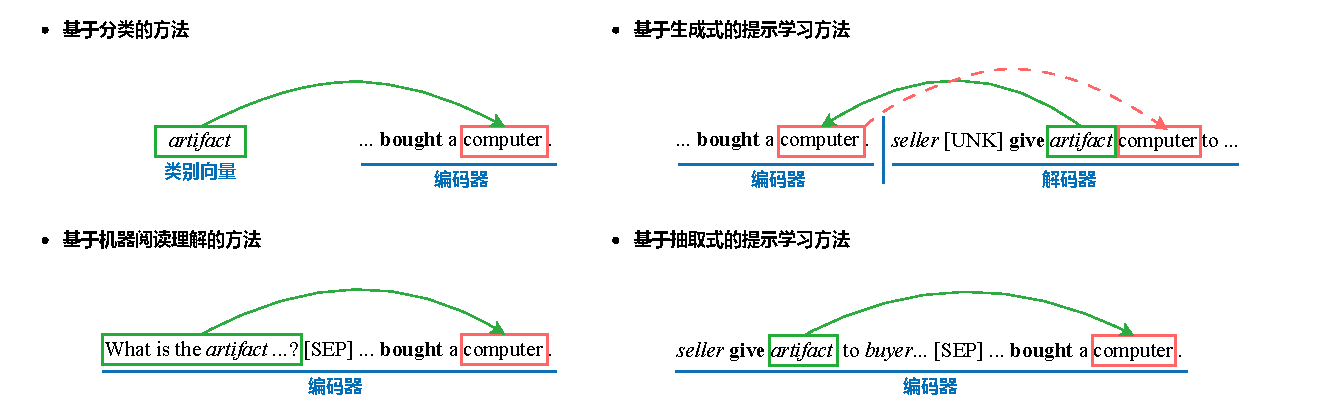
\includegraphics[width=1\linewidth]{figures/chap2/four_cls.pdf}
   \caption{四类事件要素抽取方法示意图}
   \label{four_cls}
\end{figure}

\subsection{基于分类的方法}

基于分类的方法使用传统的分类方式,构建随机初始化的分类器进行事件要素的预测。Ma等人~\cite{ma2020resource}利用预训练语言模型获取能够感知触发词信息的序列上下文表示,并进一步设计了融入依存句法结构信息的Transformer架构,得到融合句法信息的编码表示,最后使用多分类器同时完成要素文段范围和类型的建模。具体地,其首先使用BERT编码待抽取文本,并利用BERT输入中的分隔向量(segment embedding)区分对应词是否为事件触发词。对于每个词,在其BERT输出的编码表示基础上,均串接触发词和触发词对应的事件类型等信息,以增强对于事件信息的感知。然后,根据文本的依存句法解析结果,修改Transformer中的多头自注意力机制,将每个词注意力计算中的键和值限制为与其存在依存句法关系的词,从而使得其聚焦句法关联词间的自注意力建模。最后,结合预定义要素类型和BIO标注策略,利用多分类器同时完成对事件要素的文段和类型的抽取。与Ma等人~\cite{ma2020resource}直接使用序列标注建模的方式不同,一些研究者将事件要素抽取分解为子任务依次解决。例如,Zhang等人~\cite{zhang2020two}将文档级别事件要素抽取拆解为要素头单词识别和基于头单词的文段扩充两个子问题。在要素头单词识别中,对于要素类型$r$,利用特定于$r$的双仿射注意力机制(Biaffine)\cite{dozat2018simpler}参数建模候选词作为该要素类型出现的概率:
\begin{equation}
    \textrm{Pr}_r(t, c)=\frac{\exp \textrm{Biaffine}_r\left(\boldsymbol{e}_t, \boldsymbol{e}_c\right)}{\sum_{c^{\prime} \in \mathcal{C} \cup\{\epsilon\}} \exp \textrm{Biaffine}_r\left(\boldsymbol{e}_t, \boldsymbol{e}_{c^{\prime}}\right)}
\end{equation}
其中$\boldsymbol{e}_t$和$\boldsymbol{e}_c$为事件触发词和候选词经BERT编码后得到的特征表示,$\mathcal{C}$为候选词集合,$\epsilon$表示要素类型$r$不存在对应要素。而在获取头单词后,根据设置的最大要素文段长度,枚举所有可能的候选左边界和右边界词。然后,将基于头单词的文段扩充子问题转化为寻找包含该头单词的左右边界词问题,并视每个候选边界词为一个类别,构建两个多分类任务分别建模。同样地,Xu等人~\cite{xu2022two}将文档级别事件要素抽取转化为要素边界识别和要素类型分类两个子任务依次进行建模。在要素边界识别任务中,使用两个不同的BERT编码器捕捉局部和全局上下文信息。其中,局部信息的编码通过遮掩跨句词间的注意力计算得到。进一步,为了在局部信息中融入更加丰富的语义结构知识,其基于抽象语义表示(Abstract Meaning Representation,AMR)\cite{banarescu2013abstract}的解析结果,使用GCN对于局部编码表示进行语义关联信息的聚合。最后,基于门控机制融合包含了语义结构知识的局部信息和文档全局信息,并使用两个二分类损失构建要素边界的识别。而在要素类型分类中,同时使用触发词、事件类型、识别出的要素以及要素与触发词间的交互等信息进行要素类别的判断。此外,Liu等人~\cite{liu2023enhancing}将事件要素抽取转化为基于枚举文段的分类问题。具体地,其使用BERT或RoBERTa模型联合编码事件信息、待抽取文本和事件相关的要素类型信息,并对于给定的枚举文段,使用同时与该文段和事件触发词存在相关性的上下文和要素类型信息作为其整体表示。在此基础上,一方面根据对应的边界表示构建二分类边界损失,另一方面融合整体表示、边界表示和事件触发词表示等信息,构建事件要素类型的多分类损失。

\subsection{基于机器阅读理解的方法}

本类方法为每个要素类型构建相应的问题,将抽取对应要素转变为机器阅读理解(Machine Reading Comprehension,MRC)\cite{rajpurkar2016squad}问题,其能够同时获取要素的边界和类型信息,并利用到要素类型本身的语义知识。Du等人~\cite{du2020event}探索了三种不同的要素类型问题模版,包括只使用要素类型名称、结合要素类型名称与对应语义类型的疑问词、结合ACE项目中关于要素类型的标注指南与对应疑问词。然后,使用BERT对待抽取文本和问题模版进行联合编码,并参照传统的MRC方法构建要素开头和要素结尾的查询向量,使用softmax归一化建模文本中每个词分别为要素开始词和要素结尾词的概率。由于给定要素类型可能不存在或存在多个事件要素,在要素边界推断时需人为设置预测阈值。为此,其进一步根据验证集设计启发式算法,以动态决定划分要素文段和非要素文段边界概率值的最佳阈值。同样地,Li等人~\cite{li2020event}设计了包含事件触发词、事件类型和待抽取的要素类型等信息的模版作为MRC中的对应问题。为了抽取可能存在的多个事件要素,其根据每个词的编码表示构建BIO的三分类器,以替代Du等人~\cite{du2020event}采用预测阈值的做法。与Du等人~\cite{du2020event}和Li等人~\cite{li2020event}基于规则模版构建问题不同,Liu等人~\cite{liu2020event}利用无监督问题生成技术,获取与待抽取文本上下文和主题相关的自然语言表达的问题,以提升MRC模型获取答案的能力。其无监督问题生成主要包括两个部分:问题主题生成和问题上下文生成。问题主题生成与Du等人~\cite{du2020event}的设置相似,通过要素类型的语义类型使用不同的疑问词作为问题开端。而在问题上下文生成中,设计两个不同的编码器-解码器架构,以分别学习陈述性文本映射到问题描述和对应的相反映射。进一步,构建由大规模陈述性文本和未对齐的问题组成的数据语料,利用领域内自编码、去噪自编码和跨领域在线还原翻译任务进行训练。最后,使用将陈述性文本映射到对应问题的编码器-解码器模型生成待抽取文本对应的问题上下文。Zhou等人~\cite{zhou2021role}根据要素文段识别和要素类型识别分别构建两个对偶的MRC任务,通过参数共享和联合训练,实现相互协作,以提升建模性能。具体地,基于BERT分别编码待抽取文本、由要素文段和要素类型转换的问题,并利用流动注意力模块~\cite{seo2016bidirectional}实现问题表示和待抽取文本表示的交互。

进一步,一些研究利用MRC技术解决文档级别事件要素抽取带来的新问题与挑战。例如,Liu等人~\cite{liu2021machine}为了解决文档中存在的事件数据稀疏问题,利用MRC实现两种不同的数据增广。一方面,利用机器阅读理解、语义角色标注~\cite{atkins2003contribution}和事件要素抽取的跨任务数据集进行MRC模型的预训练,实现相似任务中隐式知识的传递。另一方面,使用预训练后的模型对无标注信息的文档进行事件要素信息的标注,以生成事件要素抽取任务中的更多数据实例。Wei等人~\cite{wei2021trigger}考虑到文档数据中事件要素可能分布在不同句子中,使得模型无法较好地捕捉事件触发词与要素间的长距离依赖以及事件要素间的隐式关联。为此,其在MRC模型中引入知识蒸馏技术,以提升模型在长范围文本场景下的事件内部推理和依赖知识建模能力。具体地,在其知识蒸馏框架中,对于每个要素类型,在教师网络的输入中引入事件内其他要素文段和类型信息,并使用MRC进行对应要素文段的建模。而在学生网络中,同样构建MRC抽取要素文段。基于此,从特征表示和预测概率分布两种角度将教师网络中引入的相关要素知识迁移到学生网络中。

% 进一步,采用输入中包含不同相关要素信息的多教师网络策略以提供学生网络学习到多视角知识,并基于课程学习技术逐步增加学生网络与教师网络输入不同的训练实例比例,以增强学生网络的学习效率。

此外,存在研究工作利用序列到序列框架直接生成对应的要素文段,以替代从文本中建模要素文段的范围。例如,Lu等人~\cite{lu2023event}首先构建问题生成模型,为每个要素类型获取包含了其他要素信息的问题,然后基于BART或T5~\cite{raffel2020exploring}模型生成所有归属该要素类型的要素文段。其问题生成模型同样基于BART或T5构建,输入序列为待抽取文本,对应输出序列则融合了ACE项目中关于目标要素类型的标注指南和待抽取文本中存在的其他要素文段信息。

% 采取了与Liu等人~\cite{liu2020event}类似的方法,以生成与待抽取文本相关的动态模版。为此,构建输入序列为待抽取文本,对应输出序列则融合了ACE项目中的关于目标要素类型的标注指南和待抽取文本中存在的其他要素文段信息,同样使用BART或T5进行建模。

\subsection{基于生成式的提示学习方法}

本类方法构建提示模版,利用序列到序列模型生成待抽取的事件要素信息,其相比基于机器阅读理解的方法,能够更加直接地同时抽取多个具有相同要素类型的事件要素。Li等人~\cite{li2021document}将文档级别事件要素抽取建模为基于提示模版进行填空的条件生成任务。其使用的提示模版为数据标注时参照的事件本体模版,并将模版中具体的要素类型名称替换为特殊占位符,即挖空操作。进一步,将经过挖空的提示模版和文本串接后输入到BART模型的编码器中,并在解码器中依次建模已完成要素文段填空后的提示模版序列。然后,比对填空的文段内容和对应被挖空的要素类型名称,实现要素信息的抽取。若挖空槽位的所属要素类型对应文本中多个要素文段,则在解码时使用“and”进行串联。Zeng等人~\cite{zeng2022ea2e}使用了和Li等人~\cite{li2021document}完全相同的模型架构和提示模版进行文档级别的事件要素抽取。不同的是,其在此基础上对于每个输入文本同时构建一个标注了相邻事件要素类型标签的信息增广文本,并通过对齐这两种输入文本中事件要素的编码表示,使得模型更好地感知跨事件要素的语义一致性。

类似地,Hsu等人~\cite{hsu2022degree}使用序列生成模型构建适用于不同级别文本的事件要素抽取。其与Li等人~\cite{li2021document}的研究工作相比,主要存在以下不同:(1)在构造提示模版时融合了更丰富的事件信息,包括事件类型定义和与事件语义密切相关的关键词。(2)在对事件提示模版进行挖空时,使用自然语言词汇如“some attacker”、“some organization”等替代Li等人~\cite{li2021document}使用的特殊词符进行占位。该设计使得模型可以更好地学习到要素类型的语义信息和事件整体结构信息。(3)基于人工设计进行事件提示模版的构造,未直接利用数据集中的事件本体模版知识。在序列生成模型的基础上,Hsu等人~\cite{hsu2023ampere}进一步利用AMR语义图知识。其将文本的AMR语义解析图转化为线性序列,并编码表示为若干向量表示,添加到模型Transformer架构的键向量和值向量中,从而实现结构化图知识与自然语言文本的异质融合。

进一步,Du等人~\cite{du2022dynamic}研究当文档中存在较多事件时,在序列生成模型中利用已预测的跨事件知识进行信息增益。在预测目标事件时,使用预训练的文本相似度衡量模型S-BERT~\cite{reimers2019sentence}检索出最相关的已预测事件序列,并作为额外的记忆知识和文本以及事件提示模版串接输入到生成模型的编码器中,为目标事件的要素抽取提供跨事件信息。而当预测下一个事件的要素时,根据当前目标事件要素抽取结果转化的事件序列信息将同样参与到相似度检索中,从而不断丰富待检索的事件知识。进一步,Ren等人~\cite{ren2023retrieve}研究在序列生成框架中利用多种检索增强策略提升事件要素抽取性能,包括上下文一致检索、模式一致检索和自适应混合检索。其中,上下文一致检索策略与Du等人~\cite{du2022dynamic}采用的方法相似,模式一致检索策略利用事件类型标签进行检索查询,而最后一种策略则采用连续空间中的伪示例采样进一步提升序列生成模型的类比能力。

% 此外,Zhang等人~\cite{}使用序列生成模型建模事件要素抽取的同时,利用跨数据集中的重叠知识增强模型在目标数据集的性能。训练过程可分为两大阶段:重叠知识学习阶段和特定知识学习阶段。在第一阶段中,构建一个通用的事件描述提示模版,其中包含不同的特殊占位符用于表示对应的实体类型。其训练目标为给定该通用模版及不同数据集中的待抽取文本,模型能够生成将相应事件要素填充到对应的实体类型占位符位置的序列。为了更好地存储学习到的重叠知识,该阶段在每一层Transformer的输入中均引入若干前缀向量进行训练学习并在之后阶段进行冻结。而在第二阶段,针对目标数据集的特定事件提示模版,将其中被“挖空”的事件要素类型映射到合适的实体类型占位符上,同样训练模型生成将相应事件要素填充到对应的实体类型占位符位置的序列。因而,通过实体类型与要素类型之间的映射,实现了跨数据集的有效知识迁移。

\subsection{基于抽取式的提示学习方法}

本类方法在构建提示模版的基础上,使用模版中要素类型对应的槽位表示作为查询信息,构建与机器阅读理解相似的答案获取过程,以抽取要素文段内容。该类方法结合了MRC和提示学习的优势,较好地挖掘了预训练语言模型中的先验知识。

Ma等人~\cite{ma2022prompt}最早提出了抽取式提示学习方法,以应用于句子级别和文档级别的事件要素抽取任务,其改变了之前提示学习方法基于挖空操作构建完形填空的建模方式。对于给定事件,其使用包含了该事件中所有候选要素类型的人工设计或自动学习的提示模版,并标记各自要素类型对应的槽位词位置。然后,利用BART模型建模,
以文本作为编码器输入,事件提示模版作为解码器输入,得到融合了文本上下文信息的提示模版表示。进一步,基于标记的槽位词位置,分别获取不同要素类型对应的开头与结尾查询表示向量,而后利用MRC技术构建要素文段范围。此外,其使用了二分图匹配问题中的匈牙利算法优化多答案情况下的训练损失计算。Zhang等人~\cite{zhang2022transfer}同样将事件要素抽取任务转化为基于事件模版的槽位查询问题,使得其能够与语义角色标注任务相统一,从而利用到语义角色标注的数据集进行知识迁移,提升模型在低资源场景下的性能。与Ma等人~\cite{ma2022prompt}不同的是,其使用RoBERTa模型替代BART模型,直接对文本和事件模版进行联合编码。Nguyen等人~\cite{nguyen2023contextualized}基于Ma等人~\cite{ma2022prompt}的研究工作,提出了增加软提示模版的学习,以构建每个训练实例的定制化模版输入,实现从外部文档中获取相关的上下文信息。

此外,一些研究在抽取式提示学习方法框架内考虑跨事件信息的利用。例如,Li等人~\cite{li2023intra}在利用BART模型获取目标事件中所有要素类型表示的基础上,分别构建事件内和事件外的要素类型依赖图。其中,事件外的图基于目标事件和与其最相似的事件进行构造。在此基础上,分别利用GCN建模各自的图结构信息,并在每层GCN迭代后进行跨图表示的融合。最后,利用融合了相似事件信息的不同要素类型表示和MRC技术,获取对应的要素文段。He等人~\cite{he2023revisiting}则进一步在整个上下文范围内利用跨事件信息,将多事件的并行抽取过程转化为表格生成任务。具体地,该表格提示模版的表头为多个事件提示模版的串接,而每一个行则对应包含了事件触发词和要素类型槽位的单个事件信息。在建模中,其拆分RoBERTa模型的不同网络层分别作为编码器和解码器,以替代BART模型,并通过设计结构化感知的自注意力机制并行获取不同事件内的要素类型表示,进而实现多事件的要素抽取。

\subsection{其他方法}

最近,存在一些研究工作利用最优传输(Optimal Transport)\cite{veyseh2022document}、图的链接预测(Link Prediction)\cite{yang2023amr}和链推理(Chain Reasoning)\cite{liu2023document}等方式建模文档级别的事件要素抽取任务。此外,与事件检测任务相同,一些研究基于大语言模型评估了事件要素抽取的性能。例如,Li等人~\cite{li2023evaluating}在零样本场景下评测了ChatGPT的句子级别事件要素抽取性能,其输入由任务描述、给定事件类型对应的预定义事件要素类型集合、待抽取文本和输出格式要求等。Han等人~\cite{han2023information}构建了和Li等人~\cite{li2023evaluating}相似的输入模版,并引入ICL和COT技术,提升ChatGPT在句子级别事件要素抽取上的性能表现。然而,现有方法缺乏对更具挑战性的文档级别事件要素抽取的性能评估,本文将在章节\ref{chap:chapter5}中给出ChatGPT在不同文本级别的事件要素抽取数据集上的详细实验结果。

\section{现有研究存在的问题}

前文分别基于神经网络架构的使用类型对事件检测和给定实体提及的事件要素抽取、以及基于建模方式对未给定实体提及的事件要素抽取进行了详细的梳理。然而,即使采用了不同的神经网络架构或者建模方式,这些方法均存在各自的共性问题如下:

\textbf{(1)数据不平衡依赖带来的共性识别事件能力的下降}。现有事件检测数据集中存在事件的实例比例过小,其导致的数据不平衡依赖限制了现有基于不同网络架构的事件检测模型识别事件的能力,进而降低了整体检测的性能。虽然已有方法采用偏差损失函数~\cite{chen2018collective,yan2019event,cui2020edge}或构建识别正实例/负实例~\cite{ye2019exploiting}的辅助任务进行消解,但均需要额外的超参数,以适应不同模型架构和不同程度的数据不平衡,缺乏通用性和扩展性。

\textbf{(2)实体提及带来的共性类型信息过度依赖}。现有给定实体提及的事件要素抽取方法,尽管使用的网络架构不同,但均主要研究更好地建模实体提及与事件触发词间的上下文交互~\cite{chen2015event,wang2019hmeae,xiangyu2021capturing},从而利用实体提及带来的信息增益。然而,现有方法均忽略了实体提及的类型信息与要素类型呈现出的强关联数据特性,缺乏对于这种强关联性带来的潜在实体类型信息过度依赖问题的研究和统一解决方法。

\textbf{(3)不同级别文本中存在的共性跨事件依赖关系构建限制}。现有适用于不同级别文本的事件要素抽取主要基于未给定实体提及的定义方式进行构建,其主要类型划分如章节\ref{no_entity}所总结。大多数方法均忽略了不同事件间的依赖关系,仅有少数方法~\cite{zeng2022ea2e,du2022dynamic,he2023revisiting,li2023intra}在建模时利用了这种关联依赖进行性能增益。然而,这些方法受限于构建的提示模版质量或长范围文本等因素。因此,缺乏同时解决建模方式和跨事件信息构建与利用的通用事件要素抽取方法。

根据这些共性数据依赖挑战,本文研究通用性的应对方法。具体地,研究提升事件识别能力的通用技术,在第\ref{chap:chapter3}章中提出分类器自适应知识蒸馏的事件检测方法,以消解数据不平衡依赖;研究减少建模过程产生的实体类型信息依赖的统一思路,在第\ref{chap:chapter4}章中提出多角度实体类型过度依赖消解的事件要素抽取方法,以消解对实体类型的过度依赖;研究同时解决通用文本级别事件要素建模的内在局限和构建事件间的关联依赖,在第\ref{chap:chapter5}章中提出基于分离-融合范式的多词元链接事件要素抽取模型,以实现对跨事件信息的高效构建与利用。


















































%%==================================================
%% chapter01.tex for BIT Master Thesis
%% modified by yang yating
%% version: 0.1
%% last update: Dec 25th, 2016
%%==================================================
% \chapter{基于分类器自适应知识蒸馏的事件检测框架}
\chapter{基于分类器自适应知识蒸馏的数据不平衡依赖消解}
\label{chap:chapter3}

事件检测作为事件抽取的基础子任务,其数据集中存在严重的数据不平衡现象,限制了不同事件检测模型系统的事件识别能力。针对该问题,现有方法主要利用人工设计的损失函数减少不平衡数据产生的负面影响。然而,这些方法特定于具体的模型架构和任务设计,依赖额外超参数,阻碍了其在不同数据不平衡情况下的扩展应用。为此,本章提出了一种基于分类器自适应知识蒸馏方法,以消解数据不平衡依赖问题。实验结果证明,该方法可以通用有效地提升不同事件检测模型的性能。此外,经本章实验验证,该方法可有效迁移到其他存在数据不平衡依赖的信息抽取任务中,如关系抽取等,证明了其良好的任务普适性。

\section{引言}
随着神经网络技术的快速发展,现有事件检测方法的性能取得了显著提升。然而,事件检测数据集中不存在事件的句子过多,导致这些方法普遍遭受数据不平衡依赖的困扰。例如,在ACE2005数据集的训练集部分,超过76\%的句子文本不存在事件,由此产生的过量负实例(非事件触发词)限制了现有方法高效捕捉正实例(事件触发词)的特性,使得这些方法在识别事件时性能表现有待提升。为了消解此种依赖,一些研究工作致力于增强对于正实例特性的建模或减少过高的负实例比例产生的负面影响。例如,Dos等人~\cite{dos2015classifying}在训练中不使用负实例数据,并利用成对排序损失捕捉正实例的通用特性。Chen等人~\cite{chen2018collective}在事件检测的训练损失中引入偏置参数,使得正实例和负实例以不同的权重进行训练。Ye等人~\cite{ye2019exploiting}提出了一个多任务框架,通过增加一个额外的加权损失函数进行正负实例识别能力的学习,进而更好地捕捉正实例的特性。然而,这些方法依赖于人工设计的损失函数,其需要额外的超参数以适应不同数据集的不平衡程度差异,缺乏可扩展性。此外,这些方法只针对特定的模型架构和任务设计,缺乏通用性。因此,本章研究通用的事件检测框架,在不依赖额外超参数的情况下,自动消解数据不平衡问题。

与现有工作聚焦于调整正实例或负实例的训练权重不同,本章基于数据不平衡依赖问题影响事件检测性能的方式,研究减轻其性能影响的通用方法。根据Ye等人~\cite{ye2019exploiting}的研究工作,可知数据不平衡依赖导致现有模型易将正实例预测为负实例,反之亦然。因此,数据不平衡依赖限制了现有模型识别正负实例的能力,进而降低了整体事件检测性能。

为了提升正负实例的识别性能,本章首先定义了句子级别识别信息,其表示给定实例的所在句子中是否存在事件。例如,给定文本“Mary \underline{died} on Thursday in Memphis.”和实例“died”,已知“died”触发了$Die$事件,则其句子级别识别信息为在该句子中存在事件。若给定文本“Mary lives in Memphis.”和实例“lives”,已知其文本中不存在任何事件触发词,则其句子级别识别信息为在该句子中不存在事件。基于此,在事件检测中引入了该信息,并通过预实验评估了其在消解数据不平衡依赖导致的性能下降方面的优势。表\ref{tab:gap_event}具体展示了在不同事件检测基线模型\footnote{DMRoBERTa为本章结合DMBERT和RoBERTa~\cite{liu2019roberta}而提出的一个变体模型。}中引入句子级别识别信息后的性能变化,其中“TI”和“TC”分别表示事件触发词(正例)识别\footnote{事件触发词识别在表述上等同于事件识别。}和事件检测的F1性能指标,“TI+”和“TC+”分别表示在模型输入中引入句子级别识别信息后对应的“TI”和“TC”。可以观察到,该信息的引入使得不同事件检测基线模型的事件触发词识别性能均显著提升,且提升的识别性能进一步增强其在事件检测任务的整体性能。然而,句子级别识别信息需要根据标注的事件检测标签转化得到,因此无法在推理测试阶段进行利用。

\begin{table}[htp]
\centering
\caption{ACE2005数据集上引入句子级别识别信息在F1(\%)指标上的结果对比}
\begin{tabular}{l|cccc}
\toprule
模型  & TI   & TI+  & TC   & TC+  \\ \midrule
Bi-LSTM~\cite{hochreiter1997long} & 70.1 & 78.6 & 67.8 & 71.7 \\
JMEE~\cite{liu2018jointly}    & 75.2 & 79.4 & 72.8 & 75.4 \\
MOGANED~\cite{yan2019event} & 75.9 & 79.8 & 73.4 & 76.6 \\
% EE-GCN~\cite{cui2020edge} & 78.3 & 81.8 & 77.6 & 79.2 \\
DMBERT~\cite{wang2019adversarial} & 79.4 & 84.4 & 74.6 & 80.0 \\ 
DMRoBERTa & 80.1 & 85.5 & 75.5 & 81.9 \\ \bottomrule
\end{tabular}
\label{tab:gap_event}
\end{table}

为了解决该挑战,本章构建两种网络,分别采用两类不同的输入,其主要区别为是否引入了句子级别识别信息,并实现这两种网络间的知识引导,从而弥补句子级别识别信息在不同阶段的获取差异。因此,本章进一步考虑利用知识蒸馏技术解决。传统的知识蒸馏~\cite{hinton2015distilling}将教师网络输出的软标签分布作为学生网络的监督信息,以实现将知识从教师网络转移到学生网络。然而,事件检测数据集中负实例的比例过高,导致教师网络的软标签分布中包含的正实例信息较少,知识利用效率较低。

为此,本章提出了基于分类器自适应知识蒸馏的数据不平衡依赖消解方法(Clas-

\noindent sifier-Adaptation Knowledge Distillation,CAKD),有效提升不同事件检测基线模型的性能。首先,根据训练实例的标签转化得到对应的句子级别识别信息,并作为事件识别增强网络输入的一部分参与训练,并在训练完成后固定其对应的分类器参数。然后,移除输入中的句子级别识别信息以训练事件检测网络,并共享固定的事件识别增强网络的分类器参数。通过设置额外的训练任务,使得该分类器参数引导事件检测网络从原始文本中自动学习句子级别识别信息,从而提高触发词识别任务性能并进一步增强事件检测的性能。本章的主要贡献如下:
\begin{enumerate}
    \item 研究数据不平衡依赖问题影响事件检测性能的方式,引入了句子级别识别信息消解其导致的性能下降。
    \item 提出了一种分类器自适应知识蒸馏的事件检测通用方法,自动捕捉句子级别识别信息,以消解数据不平衡依赖。
    \item 基于多种事件检测基线模型,在ACE2005数据集上进行了充分的实验。实验结果表明,本章提出的方法能够通用有效地提升不同模型的事件检测性能。
    \item 将本章提出的方法应用到同样存在数据不平衡依赖问题的关系抽取任务上,基于TACRED数据集的实验证明了其在信息抽取任务上良好的扩展性。
\end{enumerate}

\section{方法设计}
遵循最近的研究工作,给定$n$个词组成的句子实例$\left\{w_{1}, w_{2}, \cdots, w_{n}\right\}$,事件检测任务旨在为每个词$w_{i} \left(1 \leq i \leq n\right)$分配预定义的事件类型标签(包括特殊事件类型$None$,其表示对应的词不为事件触发词)。

本章提出的基于分类器自适应知识蒸馏的数据不平衡依赖消解方法主要由事件识别增强网络和事件检测网络组成,可应用于不同的事件检测基线模型。图\ref{framework_cakd}展示了基于DMBERT基线模型的CAKD方法架构。接下来,本章将作具体介绍。

% 在事件识别增强网络中,根据基线模型类型的不同,在其输入部分增加句子级别识别向量或特殊词元,以在其训练过程中引入句子级别识别信息。然后,冻结事件识别增强网络的分类器参数,进行事件检测网络的学习训练。一方面,通过共享事件识别增强网络分类器,使得句子级别识别信息可以从事件识别增强网络转移到事件检测网络,引导事件检测网络自动从原始句子中捕获句子级识别信息。同时,事件检测网络学习训练另一个分类器,用于最终的事件检测的结果预测。接下来,本章将具体介绍所提框架。

\begin{figure}[htp]
    \centering
   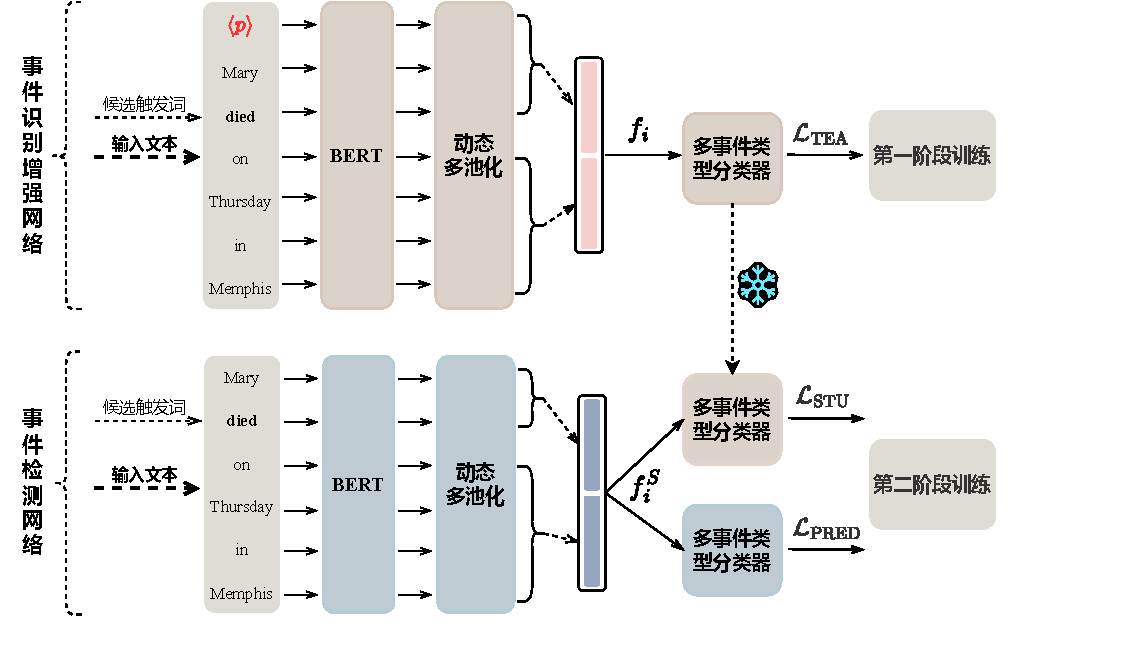
\includegraphics[width=1\linewidth]{figures/chap3/framework_cakd.pdf}
   \caption{基于DMBERT的CAKD方法架构图}
   \label{framework_cakd}
\end{figure}

\subsection{事件识别增强网络}

事件识别增强网络旨在在训练中引入句子级别识别信息,该信息可根据训练集的事件标签直接获取,不依赖于任何外部知识或资源。具体地,首先根据句子中是否存在事件触发词,将该句子标记为“\emph{Positive}”或“\emph{Negative}”。如果句子中不存在任何事件触发词,则该句子被标记为“\emph{Negative}”。如果至少存在一个事件触发词,则该句子被标记为“\emph{Positive}”。然后,基于在事件识别增强网络中使用的事件检测基线模型的类型,采用两种不同的方式在输入部分引入句子级别识别信息并进行相应编码,分别为:

\textbf{基于预训练词向量的事件检测模型}~对于句子中任意一个词$w_{i} \left(1 \leq i \leq n\right)$,首先拼接以下两类向量,表示为$\boldsymbol{x}_{i}$:
\begin{itemize}
    \item \textbf{原始输入向量}~采用其事件检测基线模型的原始输入设置。不同基线模型的输入向量有所差别,通常由预训练词向量、实体类型向量、词性标注向量和位置向量中的全部或部分串接得到。
    \item \textbf{句子级别识别向量}~通过随机初始化得到两个向量$\boldsymbol{s}_P$和$\boldsymbol{s}_N$,用于提供句子级别识别信息。若词$w_{i}$所在句子被标记为“\emph{Positive}”,则$w_{i}$对应的句子级别识别向量为$\boldsymbol{s}_P$,否则其对应的句子级别识别向量为$\boldsymbol{s}_N$。
\end{itemize}
然后,使用事件检测基线模型对输入$\boldsymbol{X}_\textrm{teacher} = (\boldsymbol{x}_{1}, \cdots, \boldsymbol{x}_{n})$进行编码。为了描述方便,本章选取Bi-LSTM~\cite{hochreiter1997long}作为基线模型,得到编码表示$\boldsymbol{f}_i \in {\mathbb{R}}^{d_{out}}$如下:
\begin{equation}
\label{eq3_1}
\boldsymbol{f}_i=\left[\overrightarrow{LSTM}\left(\boldsymbol{x}_{i}\right) ; \overleftarrow{LSTM}\left(\boldsymbol{x}_{i}\right)\right]
\end{equation} 

\textbf{基于预训练语言模型的事件检测模型}~对于句子中任意一个词$w_{i} \left(1 \leq i \leq n\right)$,首先根据句子级别识别信息在所在句子中插入可训练学习的特殊词元。具体地,若词$w_{i}$所在句子被标记为“\emph{Positive}”,则在句首插入特殊词元$\langle p \rangle$,否则在句首插入特殊词元$\langle n \rangle$。假设句首插入的特殊词元为$\langle p \rangle$,且选取DMBERT~\cite{wang2019adversarial}作为事件检测基线模型,则首先使用BERT~\cite{devlin2019bert}进行编码,得到特征表示如下:
\begin{equation}
  \left\{\boldsymbol{s}_P,\boldsymbol{h}_{1},\cdots,\boldsymbol{h}_{j},\cdots,\boldsymbol{h}_{n}\right\}=\textrm{BERT}(\langle p \rangle, w_{1},\cdots, w_{j},\cdots, w_{n})
\end{equation}
其中$\boldsymbol{s}_P$为$\langle p \rangle$对应的特征表示,$\boldsymbol{h}_{j} \left(1 \leq j \leq n\right)$为${w}_{j} \left(1 \leq j \leq n\right)$对应的特征表示。在此之后,使用一个动态多池化操作分段聚合编码后的特征表示:
\begin{equation}
    \left[\boldsymbol{h}_{1, i}\right]_{k}=\max \left\{\left[\boldsymbol{s}_P\right]_{k}, \left[\boldsymbol{h}_{1}\right]_{k} \cdots,\left[\boldsymbol{h}_{i}\right]_{k}\right\}
\end{equation}
\begin{equation}
    \left[\boldsymbol{{h}}_{i+1, n}\right]_{k}=\max \left\{\left[\boldsymbol{h}_{i+1}\right]_{k} \cdots,\left[\boldsymbol{h}_{n}\right]_{k}\right\}
\end{equation}
其中$[\cdot]_{k}$表示一个向量的第$k$个元素值。最后,串接上述表示得到$w_{i}$的特征表示$\boldsymbol{f}_i \in {\mathbb{R}}^{d_{out}}$:
\begin{equation}
\label{input_information}
\boldsymbol{f}_i=\left[\boldsymbol{h}_{1, i};\boldsymbol{{h}}_{i+1, n}\right]
\end{equation}

然后,对于不同类型的事件检测基线模型,将特征表示$\boldsymbol{f}_i$输入到多事件类别分类器,以计算概率分布$p\left(w_{i}\right)$如下:
\begin{equation}
  p\left(w_{i}\right) = \textrm{softmax}\left(\boldsymbol{W}_{S}\boldsymbol{f}_i + \boldsymbol{b}_{S}\right)
\end{equation}
其中$\boldsymbol{W}_{S} \in {\mathbb{R}}^{C \times d_{out}}$和$\boldsymbol{b}_{S} \in {\mathbb{R}}^{C}$表示分类器中需要学习训练的参数,其中$C$为预定义的事件类型数目。假设给定的批数据$\mathcal{B}$中存在$K$个词,其交叉熵损失$\mathcal{L_\textrm{TEA}}$计算如下:
\begin{equation}
  \mathcal{L_\textrm{TEA}} = -\sum^{K} \log p\left(e|w_{i}\right)
 \label{ce}
\end{equation}
其中$p\left(e|w_{i}\right)$表示事件识别增强网络将词$w_{i}$预测为正确的事件类型$e$的概率值。

\subsection{事件检测网络}

事件检测网络旨在建模事件检测任务,其使用原始的文本信息作为输入。然后,一方面基于固定的事件识别增强网络分类器参数设计辅助训练任务,引导事件检测网络自动从原始文本中捕获句子级别识别信息。同时,学习训练另一个分类器,以用于事件类型预测。

在事件检测网络输入部分,若使用基于预训练词向量的事件检测模型如Bi-LSTM进行编码,则移除$\boldsymbol{X}_\textrm{teacher} = (\boldsymbol{x}_{1}, \cdots, \boldsymbol{x}_{n})$中拼接的句子级别识别向量$\boldsymbol{s}_P$或$\boldsymbol{s}_N$,记作$\boldsymbol{X}_\textrm{student} = (\boldsymbol{x}_{1}^{S}, \cdots, \boldsymbol{x}_{n}^{S})$。然后,利用另一个Bi-LSTM~\cite{hochreiter1997long}得到编码表示$\boldsymbol{f}_i^{S} \in {\mathbb{R}}^{d_{out}}$如下:
\begin{equation}
\label{eq3_8}
\boldsymbol{f}_i^{S}=\left[\overrightarrow{LSTM}\left(\boldsymbol{x}_{i}^{S}\right) ; \overleftarrow{LSTM}\left(\boldsymbol{x}_{i}^{S}\right)\right]
\end{equation}

若使用基于预训练语言模型的事件检测模型如DMBERT,则首先利用另一个BERT编码不包含特殊词元$\langle p \rangle$或$\langle n \rangle$的原始文本:

\begin{equation}
  \left\{\boldsymbol{h}_{1}^{S},\cdots,\boldsymbol{h}_{j}^{S},\cdots,\boldsymbol{h}_{n}^{S}\right\}=\textrm{BERT}(w_{1},\cdots, w_{j},\cdots, w_{n})
\end{equation}
在此之后,同样使用一个动态多池化操作分段聚合编码后的特征表示,并进一步串接得到$\boldsymbol{f}_i^{S} \in {\mathbb{R}}^{d_{out}}$:
\begin{equation}
    \left[\boldsymbol{h}_{1, i}^{S}\right]_{k}=\max \left\{\left[\boldsymbol{h}_{1}^{S}\right]_{k} \cdots,\left[\boldsymbol{h}_{i}^{S}\right]_{k}\right\}
\end{equation}
\begin{equation}
    \left[\boldsymbol{{h}}_{i+1, n}^{S}\right]_{k}=\max \left\{\left[\boldsymbol{h}_{i+1}^{S}\right]_{k} \cdots,\left[\boldsymbol{h}_{n}^{S}\right]_{k}\right\}
\end{equation}
\begin{equation}
\label{input_information}
\boldsymbol{f}_i^{S}=\left[\boldsymbol{h}_{1, i}^{S};\boldsymbol{{h}}_{i+1, n}^{S}\right]
\end{equation}

然后,对于不同类型的事件检测基线模型,将特征表示$\boldsymbol{f}_i^{S}$输入到事件识别增强网络分类器中,计算概率分布$p^{S}\left(w_{i}\right)$如下:
\begin{equation}
  p^{S}\left(w_{i}\right) = \textrm{softmax}\left(\boldsymbol{W}_{S}\boldsymbol{f}_i^{S} + \boldsymbol{b}_{S}\right)
\end{equation}
给定包含$K$个词的批数据$\mathcal{B}$,其交叉熵损失$\mathcal{L_\textrm{STU}}$计算如下:
\begin{equation}
  \mathcal{L_\textrm{STU}} = -\sum^{K} \log p^{S}\left(e|w_{i}\right)
\end{equation}
其中$p^{S}\left(e|w_{i}\right)$表示将词$w_{i}$预测为正确的事件类型$e$的概率值。同时,将特征表示$\boldsymbol{f}_i^{S}$输入到另一个多事件类别分类器中,得到概率分布$p^{E}\left(w_{i}\right)$如下:
\begin{equation}
  p^{E}\left(w_{i}\right) = \textrm{softmax}\left(\boldsymbol{W}_{E}\boldsymbol{f}_i^{S} + \boldsymbol{b}_{E}\right)
\end{equation}
其中$\boldsymbol{W}_{E} \in {\mathbb{R}}^{C \times d_{out}}$和$\boldsymbol{b}_{E} \in {\mathbb{R}}^{C}$表示该分类器中需要训练的参数。给定包含$K$个词的批数据$\mathcal{B}$,则其交叉熵损失$\mathcal{L_\textrm{PRED}}$计算如下:
\begin{equation}
  \mathcal{L_\textrm{PRED}} = -\sum^{K} \log p^{E}\left(e|w_{i}\right)
 \label{ce}
\end{equation}
其中$p^{E}\left(e|w_{i}\right)$表示事件检测网络将词$w_{i}$预测为正确的事件类型$e$的概率值。

\subsection{训练和推理}
在训练阶段,首先基于损失$\mathcal{L_\textrm{TEA}}$训练事件识别增强网络。在完成事件识别增强网络训练后,固定其分类器参数$\boldsymbol{W}_{S}$和$\boldsymbol{b}_{S}$,并基于如下损失训练事件检测网络:
\begin{equation}
  \mathcal{L_\textrm{OVERALL}} = \mathcal{L_\textrm{STU}} + \mathcal{L_\textrm{PRED}}
  \label{overall_stu}
\end{equation}
其中最小化$\mathcal{L_\textrm{STU}}$能够在训练过程中通过共享固定的事件识别增强网络参数$\boldsymbol{W}_{S}$和$\boldsymbol{b}_{S}$,引导事件检测网络自动从文本中捕获句子级别识别信息。同时,最小化$\mathcal{L_\textrm{PRED}}$使得参数$\boldsymbol{W}_{E}$和$\boldsymbol{b}_{E}$聚焦于事件类型的分类建模。在推理阶段,使用$p^{E}\left(w_{i}\right)$获取$w_{i}$对应的事件类型。

\section{实验评估}

\subsection{实验设置}
\label{experiment_settings}
\textbf{1.数据集}~对于事件检测任务,本章使用了包含599个文档和33种事件类型的ACE2005语料库~\cite{doddington2004automatic},该语料库数据来源为报纸、新闻专线数据和广播新闻,由自动内容提取项目(Automatic Content Extraction,ACE)完成标注。其存在英文、中文和阿拉伯文版本,遵循最近的研究工作~\cite{chen2015event,lu2019distilling},本章使用英文版本(以下简称ACE2005数据集),并分别使用了529、40和30个文档作为训练集、验证集和测试集。此外,在训练集中,仅3325个句子存在至少一种事件,而剩余的10594个句子中不存在任何事件,因此其数据不平衡问题显著。

\textbf{2.评价指标}~本章实验遵循事件检测任务的标准评估~\cite{li2013joint,chen2015event}。如果事件触发词和对应的事件类型均与数据集标注的信息完全相同,则认定该事件触发词被正确检测,本章模型采用包括特殊事件类型$None$(空)的多分类方式同时识别事件触发词和预测对应的事件类型。
基于此,本章使用不区分事件类别的微平均方式计算准确率(P)、召回率(R)和F1值(F1)作为评估指标,具体如下:
\begin{equation}
   P=\frac{TP}{TP+FP}
\end{equation}
\begin{equation}
   R=\frac{TP}{TP+FN}
\end{equation}
\begin{equation}
   F1=\frac{2 \times P \times R}{P+R} 
\end{equation}
其中$TP$为检测出的正确事件触发词数目,$FP$为检测出的错误事件触发词数目,而$FN$则表示未被检测出的事件触发词数目。

\textbf{3.基线方法}~本节选择以下方法参与实验比较,这些方法均可基于不同的事件检测基线模型进行性能评估,具体包括:
\begin{itemize}
    \item \textbf{基线模型}:仅利用$\mathcal{L_\textrm{PRED}}$训练事件检测网络,其退化为对应的事件检测模型。
    \item \textbf{基线模型+Sim-CAKD}:本章提出的CAKD方法的简化版本。具体地,事件检测网络不额外学习训练新的多事件类别分类器,而直接利用事件识别增强网络的分类器进行事件类型的建模。因此,公式~\ref{overall_stu}中$\mathcal{L_\textrm{OVERALL}} = \mathcal{L_\textrm{STU}}$。在推理阶段,同样利用事件识别增强网络的分类器获取事件检测任务的结果。
    \item \textbf{基线模型+MTL}:遵循Ye等人~\cite{ye2019exploiting}消解关系抽取中数据不平衡依赖的思路,通过共享网络编码,增加额外的事件触发词识别任务,采用多任务学习方式进行建模。下文将介绍关键细节。
\end{itemize}

对于基线模型+MTL方法,假设给定句子中任意一个词$w_{i} \left(1 \leq i \leq n\right)$,根据选定的事件检测基线模型编码得到特征表示为$\boldsymbol{f}_i^{M}$。在事件触发词识别任务中,计算对应的二分类损失$\mathcal{L_\textrm{ID}}$如下:
\begin{equation}
  p^{I}\left(w_{i}\right) = \sigma\left(\boldsymbol{W}_{I}\boldsymbol{f}_i^{M} + \boldsymbol{b}_{I}\right)
\end{equation}
\begin{equation}
    \mathcal{L_\textrm{ID}} = - \sum^{K} \left(L_{i} \log p^{I}\left(w_{i}\right) + (1-L_{i}) \log \left(1-p^{I}\left(w_{i}\right)\right) \right)
\end{equation}
其中$\boldsymbol{W}_{I} \in {\mathbb{R}}^{1 \times d_{out}}$和$\boldsymbol{b}_{I} \in {\mathbb{R}}^{1}$分别表示该二分类器的训练参数,$\sigma(\cdot)$为sigmoid激活函数。当词$w_{i}$为事件触发词,则$L_{i}$设置为1,否则设置为0。而在事件检测任务中,将特征表示$\boldsymbol{f}_i^{M}$输入到多事件类别分类器中,得到对应的事件检测任务损失$\mathcal{L_\textrm{CL}}$:
\begin{equation}
  p^{C}\left(w_{i}\right) = \textrm{softmax}\left(\boldsymbol{W}_{C}\boldsymbol{f}_i^{M} + \boldsymbol{b}_{C}\right)
\end{equation}
\begin{equation}
  \mathcal{L_\textrm{CL}} = -\sum^{K} \log p^{C}\left(e|w_{i}\right)
 \label{ce}
\end{equation}
其中$\boldsymbol{W}_{C} \in {\mathbb{R}}^{C \times d_{out}}$和$\boldsymbol{b}_{C} \in {\mathbb{R}}^{C}$表示该分类器中需要训练的参数。基于损失$\mathcal{L_\textrm{ID}}$和$\mathcal{L}_\textrm{CL}$,则可得该多任务学习方法的总训练损失:
\begin{equation}    \mathcal{L}_\textrm{M}=\alpha\mathcal{L}_\textrm{ID}+(1-\alpha)\mathcal{L}_\textrm{CL}
\end{equation}
其中$\alpha$为权重超参数。

在本章所提的CAKD方法和上述基线方法中,不仅使用Bi-LSTM~\cite{hochreiter1997long},还利用以下事件检测基线模型参与性能验证:(1)Liu等人提出的JMEE~\cite{liu2018jointly},其融合了自注意力机制和GCN,以编码句法结构信息和捕捉不同事件间的关联。(2)Yan等人提出的MOGANED~\cite{yan2019event},其使用GAT网络聚合依存句法树中的多跳句法信息,以有效建模非邻接依存关系。(3)Wang等人提出的DMBERT~\cite{wang2019adversarial},其将DMCNN~\cite{chen2015event}模型中的CNN替换成BERT,并保留动态多池化操作。(4)本章提出的DMRoBERTa,其将DMBERT中的BERT替换成对应的改进版预训练语言模型RoBERTa~\cite{liu2019roberta},其他部分保持不变。

\textbf{4.实验配置}~对于基于预训练词向量的事件检测模型,各自原始输入向量保持不变,一般由预训练词向量、随机初始化的实体类型标签向量、位置向量和词性标注向量等组成,而其句子级别识别向量的维度均设置为300。此类事件检测模型的实验服务器配置均为:CPU型号Intel(R) Xeon(R) Gold 5218,主频2.30GHz;内存128G;GPU计算卡型号NVIDIA GeForce RTX 1080Ti,显存11G。对于基于预训练语言模型的事件检测模型,分别加载HuggingFace上发布的“google-bert/bert-base-uncased”文件\footnote{https://huggingface.co/google-bert/bert-base-uncased}和“FacebookAI/roberta-base”文件\footnote{https://huggingface.co/FacebookAI/roberta-base}作为编码使用的BERT和RoBERTa预训练模型参数。学习率均设置为5e-5,并使用AdamW进行训练优化。此类事件检测模型的实验服务器配置均为:CPU型号Intel(R) Xeon(R) Gold 5320,主频2.20GHz;内存256G;GPU计算卡型号NVIDIA GeForce RTX 3090,显存24G。此外,对于所有事件检测模型,其第一阶段训练均采用早停策略决定训练的轮次。当事件识别增强网络连续3轮在验证集上的F1指标没有出现提升,则结束该阶段的训练。在第二阶段训练中,若使用的基线模型为Bi-LSTM,则事件检测网络的轮次设置为30。对于其他事件检测基线模型,其事件检测网络采用对应事件检测模型的训练轮次或策略\footnote{DMRoBERTa参照DMBERT的训练轮次设置。}。本章实验均基于Pytorch~\cite{paszke2017automatic}框架完成。

\subsection{性能结果}
\label{3_3_2}

表\ref{tab:event}展示了在ACE2005数据集上的事件检测实验结果,其中$*$表示重新运行其发布的源代码得到的F1指标值。可以看出,本章所提的CAKD方法可以显著增强所有事件检测基线模型的F1指标,其涵盖了基于预训练词向量和预训练语言模型两种不同的类型。其中,CAKD方法能够大幅提升基于预训练语言模型的事件检测基线模型,分别在DMBERT和DMRoBERTa的F1指标上取得了4.0\%和3.8\%的性能提升。进一步,可以观察到对于所有的事件检测基线模型,CAKD方法在F1性能指标上都超过了相应的简化方法Sim-CAKD,其证明了将预测事件类型和学习句子级别识别信息的训练参数进行分隔,能提升对应基线模型的性能。对于MTL方法,其能够提升Bi-LSTM、DMBERT和DMRoBERTa等基线模型的F1性能表现,但其性能提升幅度均不如CAKD方法。而且,在使用了GNN网络架构的JMEE和MOGANED模型上,MTL方法降低了其对应的F1指标结果。因此,相比于MTL方法,本章所提的CAKD方法表现出在不同类型基线模型上的性能优势和通用性。此外,可以发现CAKD方法在不同基线模型上均主要通过显著增强预测的召回率提高整体的F1指标。该发现可以归因于本章提出的CAKD方法能够提升基线模型自动从文本中学习句子级别识别信息的能力,以更好地获取给定实例的正负实例情况,从而在事件检测中能以更高的置信水平预测出比例较小的正例数据。与之相反,基线模型本身在缺乏获取句子级别识别信息的能力时,倾向于避免将更多的给定实例预测为正例,导致较低的召回率。

\begin{table}[htp]
\centering
    \caption{ACE2005数据集上的事件检测性能结果}
	\begin{tabular}{lccc}
		\toprule
		模型 & P(\%) & R(\%) & F1(\%)  \\
		\midrule
		Bi-LSTM            & 68.6  & 67.0  & 67.8      \\
		Bi-LSTM+MTL            & 66.4  & 70.6  & 68.4        \\
		Bi-LSTM+Sim-CAKD   & 67.2  & 71.5  & 69.3      \\
        Bi-LSTM+CAKD   & 68.2  & 71.7  & \textbf{69.6}      \\
        \midrule
	 %    Bi-GRU            & 69.4  & 68.4  & 68.9      \\
		% Bi-GRU+MTL     & 67.0  & 73.3  & 70.0        \\
		% Bi-GRU+Sim-CAKD   & 67.5  & 73.8  & 70.5      \\
  %       Bi-GRU+CAKD   & 68.1  & 76.2  & \textbf{71.9}      \\
		% \midrule
		JMEE           & 75.3  & 70.5  & 72.8$^*$      \\
		JMEE+MTL            & 71.9  & 65.3  & 68.5      \\
		JMEE+Sim-CAKD           & 74.0  & 73.1  & 73.6      \\
        JMEE+CAKD           & 75.0  & 72.4  & \textbf{73.7}      \\
        	\midrule
		MOGANED          & 81.0  & 67.0  & 73.4$^*$      \\
		MOGANED+MTL            & 76.5  & 66.1  &  70.9     \\
		MOGANED+Sim-CAKD          & 79.4  & 69.1  & 73.9     \\
        MOGANED+CAKD           & 78.7  & 72.3  & \textbf{75.4}    \\
        	\midrule
		% EE-GCN          & 76.7   & 78.6  & 77.6      \\
		% EE-GCN+MTL            & 75.5  & 75.6  &  75.5     \\
		% EE-GCN+Sim-CAKD          & 76.2  & 79.1  & 77.6     \\
  %       EE-GCN+CAKD           & 76.4  & 79.9  & \textbf{78.1}    \\ \midrule
        DMBERT & 77.6 & 71.8 & 74.6   \\
	DMBERT+MTL &  75.3 & 77.7  & 76.5    \\
	DMBERT+Sim-CAKD & 76.0  & 81.2  & 78.5 \\
        DMBERT+CAKD & 75.6  & 81.9  & \textbf{78.6}  \\ \midrule
        DMRoBERTa & 71.1 & 80.5 & 75.5   \\
	DMRoBERTa+MTL & 76.4  & 76.0  &  76.2   \\
	DMRoBERTa+Sim-CAKD & 71.6  & 85.7  & 78.0 \\
        DMRoBERTa+CAKD & 73.7  & 85.9  & \textbf{79.3}  \\
		\bottomrule
	\end{tabular}
	\label{tab:event}
\end{table}

\subsection{与基于预训练语言模型的基线性能比较}

结合本章研究工作、DMBERT~\cite{wang2019adversarial}和RoBERTa~\cite{liu2019roberta}的发表时间,本章选取基于预训练语言模型且性能表现优秀的事件检测模型与CAKD方法作性能对比,具体包括:(1)Lai等人提出的GatedGCN~\cite{lai2020event},其基于BERT进行编码,并利用依存句法树在GCN中构建候选触发词特征表示对其他单词信息的过滤筛选。(2)Tong等人提出的EKD~\cite{tong2020improving},其基于BERT进行编码,并构建知识蒸馏框架,利用从WordNet获取的开放域触发词知识提升对训练集中稀疏和未出现事件触发词的识别。(3)Veyseh等人提出的GPTEDOT~\cite{veyseh2021unleash},其基于BERT进行编码,并利用GPT-2为事件检测生成额外的训练数据。此外,考虑到ChatGPT在多种自然语言处理任务上表现优异,Han等人~\cite{han2023information}利用情境学习(In-Context Learning,ICL)~\cite{brown2020language}构建5-shot ICL提示模版作为ChatGPT的输入,以生成ACE2005数据集上所有测试样本的事件检测结果。本章展示其F1指标作为性能参考。


表\ref{sota_comparison}展示的结果表明,DMRoBERTa+CAKD在F1指标上获得了最优性能,而DMBERT+CAKD也在F1指标上超越了GatedGCN和EKD模型。此结果表明,虽然只采用了简单的预训练语言模型编码和池化操作,但在应用了本章提出的CAKD方法后,与上述引入了外部知识资源如依存句法信息、WordNet和额外生成数据的事件检测模型相比,仍表现出具有竞争力的实验结果,进一步验证了CAKD方法的性能效率。另外,可以观察到ChatGPT的输入受限于少样本场景,在事件检测任务上性能表现不佳。

\begin{table}[htp]
\centering
    \caption{ACE2005数据集上基于预训练语言模型的事件检测性能结果对比}
	\begin{tabular}{lccc}
		\toprule
		模型 & P(\%) & R(\%) & F1(\%)  \\
		\midrule
        ChatGPT & - & - & 27.3 \\
        \midrule
		GatedGCN & 78.8 & 76.3 & 77.6       \\
		EKD & 79.1 & 78.0 & 78.6  \\ 
        GPTEDOT & 82.3 & 76.3 & 79.2 \\ \midrule  
        DMBERT+CAKD & 75.6  & 81.9  & 78.6  \\ 
        DMRoBERTa+CAKD & 73.7  & 85.9  & \textbf{79.3}  \\
		\bottomrule
	\end{tabular}
	\label{sota_comparison}
\end{table}

\subsection{事件触发词识别能力分析}

% 为了证明所提出的CAKD框架可以提高基线模型识别给定实例是正还是负例的能力(即事件触发词识别能力),
本节比较CAKD方法和相应的基线模型在事件触发词识别任务上的F1性能指标。如表\ref{tab:identification_compare}所示,在不同基线模型上引入CAKD方法,其识别事件触发词的性能均显著提升,证明其能够通用地消解数据不平衡依赖问题带来的正负例识别能力的下降。

\begin{table}[htp]
    \centering
    \caption{ACE2005数据集上的事件触发词识别任务F1(\%)指标结果}
	\begin{tabular}{lcc}
	    \toprule
		模型  & 基线模型  & 基线模型+CAKD   \\
		\midrule
		Bi-LSTM   & 70.1  & 71.6      \\
		JMEE      & 75.2  &  77.2        \\
		MOGANED   & 75.9  & 78.7    \\
            % EE-GCN   & 78.3  & 79.4    \\
            DMBERT   &  79.4 &  82.8   \\
            DMRoBERTa   &  80.1 &  84.3   \\   
		\bottomrule
	\end{tabular}
	\label{tab:identification_compare}
\end{table}

\subsection{数据不平衡程度分析}

本节分析在不同程度数据不平衡场景下,CAKD方法、MTL方法以及相应的基线模型方法在事件检测任务上的性能变化。具体地,在分析实验中采用DMRoBERTa作为基线模型,并依次从ACE2005数据集训练集中随机删减等间隔数量存在事件的句子数据,以构建存在不同数据不平衡程度的训练数据。如图\ref{imbalance}所示,随着数据不平衡程度的增加,不同方法的F1指标均呈现下降趋势,但DMRoBERTa+CAKD的下降最为平缓,在不同场景下的F1指标均显著优于同样应用了数据不平衡依赖消解的DMRoBERTa+MTL,验证了本章提出的CAKD方法在消解不同数据不平衡依赖的优势。进一步,可以观察到DMRoBERTa相比于应用了数据不平衡依赖消解的DMRoBERTa+CAKD和DMRoBERTa+MTL,在更加极端的不平衡数据场景下性能劣势显著增加,表明了数据不平衡依赖消解的必要性。

\begin{figure}[htp]
    \centering
   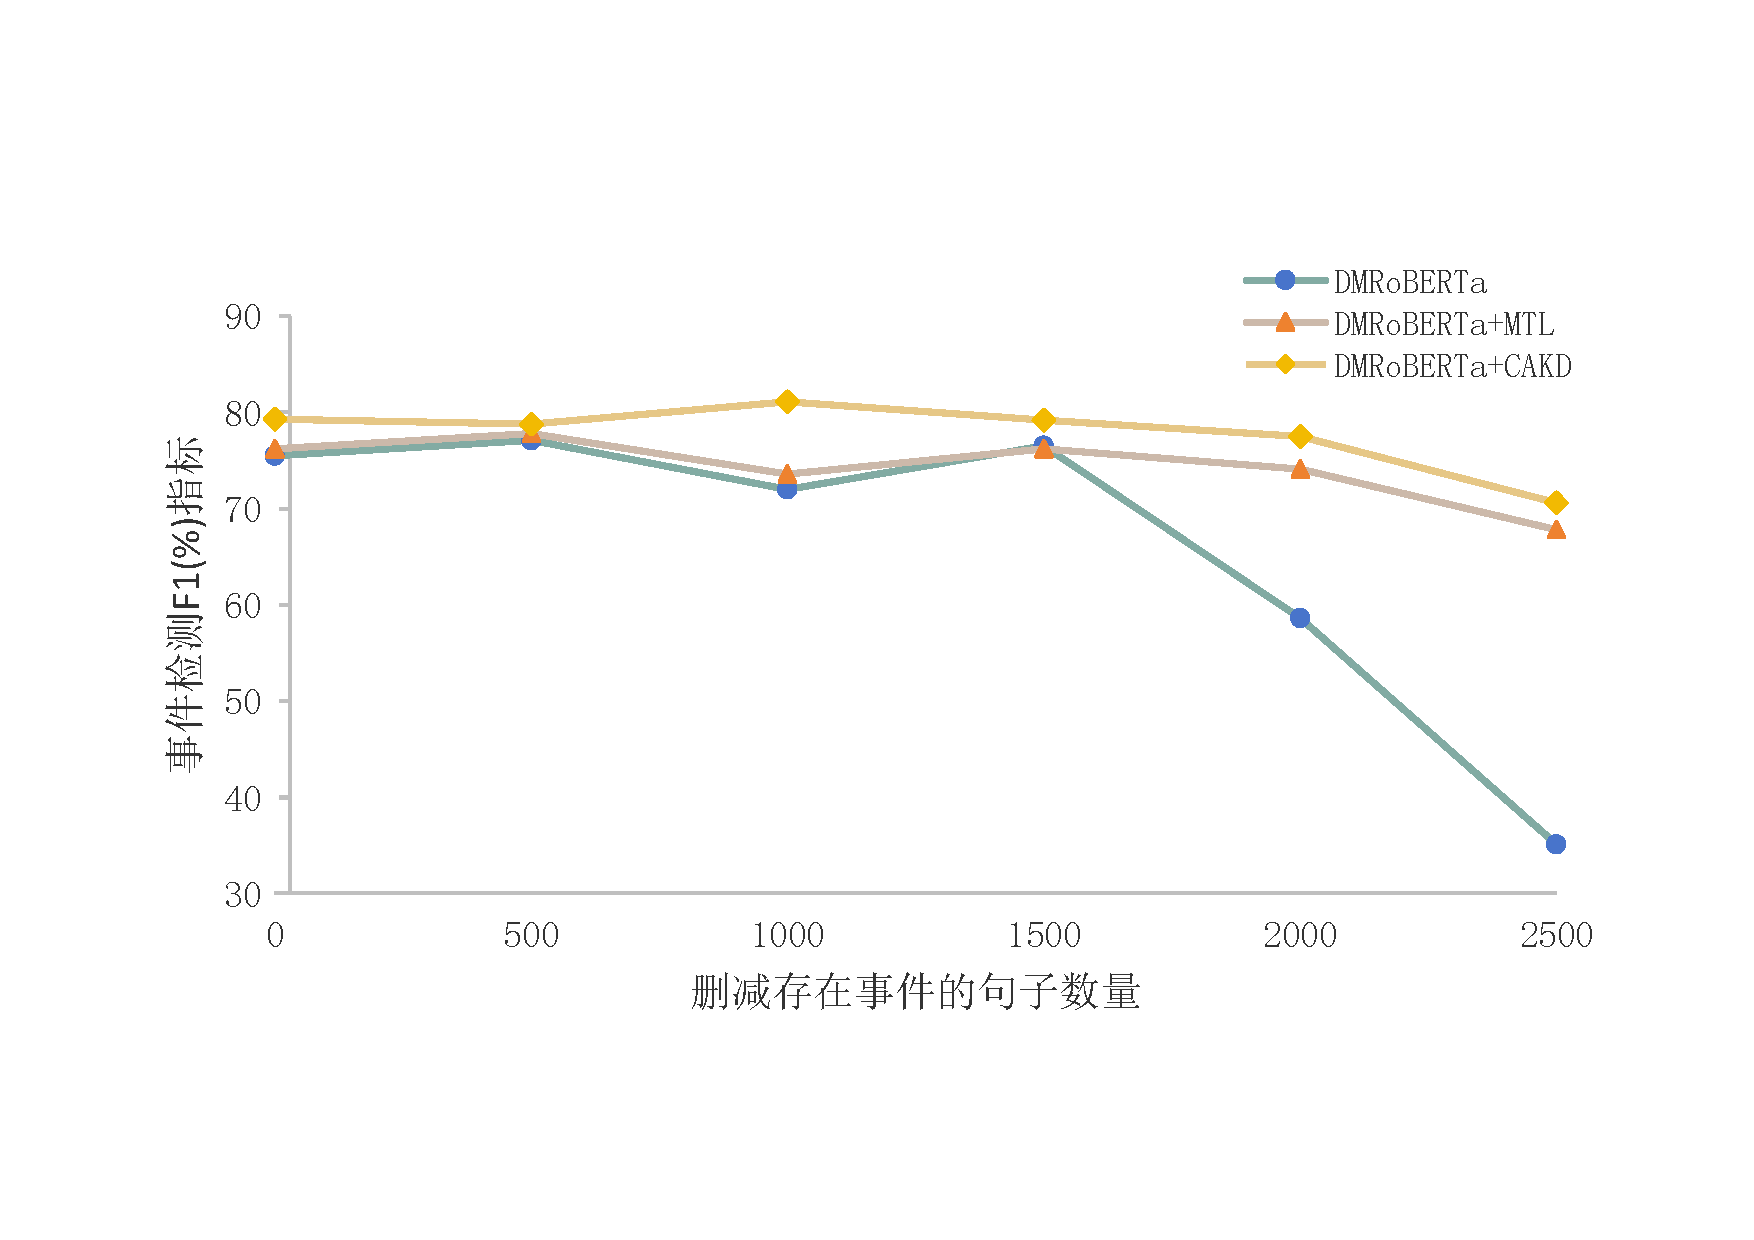
\includegraphics[width=0.8\linewidth]{figures/chap3/imbalance.pdf}
   \caption{不同程度数据不平衡下不同方法在F1(\%)指标上的结果对比}
   \label{imbalance}
\end{figure}

\subsection{案例研究}
本节基于ACE2005数据集中的具体实例进行案例分析。表\ref{case_study_event}展示了本章提出的CAKD方法和对应的基线模型在具体实例上的事件检测结果,其中粗体单词表示事件触发词,“频率”为对应事件类型的触发词占总事件触发词数目的比例。可以看到,在实例(1)中,虽然“acquitted”较为明显地触发了$Acquit$(宣判无罪)事件类型,基线模型仍由于该事件类型的稀疏性而将“acquitted”预测为非事件触发词。类似地,在实例(2)中,由于“rally”为罕见的事件触发词,基线模型无法识别出“rally”触发了$Demonstrate$(认定)事件类型。与之相比,CAKD方法能够基于文本内容建模句子级别识别信息,具备了更好地预测句子中是否存在事件的能力,相应提升了对于罕见事件类型和罕见事件触发词的识别,从而给出了正确的检测结果。

\begin{table*}[htp]
\centering
\small
\caption{ACE2005数据集上的案例分析}
\begin{tabular}{lcccc}
\toprule
\multicolumn{1}{c}{实例} & 正确事件标签 & 基线模型 & 基线模型+CAKD & 频率 \\ \midrule
\begin{tabular}[c]{@{}l@{}}(1) The Pakistani supreme court \\ last year \textbf{acquitted} Ayub Masih.\end{tabular} & Acquit & None & Acquit & 0.01\%  \\ \midrule
\begin{tabular}[c]{@{}l@{}}(2) Judge Shahid Rafiq..., found \\ Ranjha Masih guilty of defiling \\ Koranic verses during a protest \\ \textbf{rally} by the minority Christian \\ community in 1998.\end{tabular} & \multicolumn{1}{l}{Demonstrate} & None  & Demonstrate & 1.47\% \\ \bottomrule
\end{tabular}
\label{case_study_event}
\end{table*}

\subsection{其他信息抽取任务上的扩展实验}

为了进一步验证CAKD方法在其他任务上的良好扩展性,本章将CAKD方法迁移到信息抽取的另一关键任务—关系抽取上。在该任务中,数据不平衡问题同样严重存在。例如,在广泛使用的关系抽取数据集TACRED~\cite{zhang2017position}上,约80\%的实体对中不存在关系。因此,本章在TACRED数据集上比较CAKD方法和章节\ref{experiment_settings}中介绍的基线方法的性能结果。同样地,在这些方法中,使用不同的基线模型,包括Bi-LSTM、Bi-GRU、PA-LSTM~\cite{zhang2017position}、C-GCN~\cite{zhang2018graph}、C-AGGCN~\cite{guo2019attention}和GDPNet~\cite{xue2021gdpnet}。其中,在CAKD和Sim-CAKD方法中,采用和事件检测任务相似的策略,构建两个网络,在其中一个网络的输入中引入句子级别识别信息,并分别利用这些基线模型得到两个网络对应的编码表示,以替代公式\ref{eq3_1}和公式\ref{eq3_8}中的$\boldsymbol{f}_i$和$\boldsymbol{f}_i^{S}$,而方法中的其他部分则保持不变。

表\ref{relation_results}展示了在TACRED数据集上的关系抽取实验结果,其中$*$表示重新运行其发布的源代码得到的F1指标值。可以看出,将本章提出的CAKD方法迁移到不同的基线模型上,均提升了在关系抽取任务上的F1性能结果,有效地证明了本章所提方法的良好任务扩展性。同样地,其对应的简化方法Sim-CAKD也提升了不同关系抽取模型的整体性能,但其平均性能表现与CAKD方法存在一定差距,验证了与章节\ref{3_3_2}类似的结论,即分隔预测关系类型和学习句子级别识别信息的训练参数,能提升对应基线模型的性能。对于MTL方法,其能够提升Bi-LSTM和Bi-GRU模型的F1指标,但在其他关系抽取基线模型上表现不佳,进一步证明了该方法只适用于部分类型的网络架构模型。

\begin{table}[htp]
    \centering
    \caption{TACRED数据上的关系抽取性能结果}
	\begin{tabular}{lccc}
		\toprule
		模型 & P(\%) & R(\%) & F1(\%)  \\
		\midrule
		Bi-LSTM            & 65.7  & 58.9  & 62.1      \\
		Bi-LSTM+MTL            & 63.4  & 62.8  & 63.1       \\
        Bi-LSTM+Sim-CAKD            & 63.8  & 62.3  & 63.0    \\
		Bi-LSTM+CAKD   & 66.2  & 62.0  & \textbf{64.1}      \\
		\midrule
	    Bi-GRU            & 70.1 & 59.1  & 64.2      \\
		Bi-GRU+MTL     &  64.0 & 65.8  &  64.9       \\
		Bi-GRU+Sim-CAKD   &  66.7 & 64.5  &  65.6     \\
        Bi-GRU+CAKD   & 67.4 & 64.1  & \textbf{65.7}      \\
		\midrule
		PA-LSTM   & 65.7  & 64.5  & 65.1      \\
		PA-LSTM+MTL            & 66.2  & 63.4  & 64.8      \\
        PA-LSTM+Sim-CAKD            & 69.1  & 61.9  & 65.3        \\
		PA-LSTM+CAKD            & 67.1  & 66.4  & \textbf{66.7}     \\
		\midrule
		GCN            & 69.8  & 59.0  & 64.0      \\
		GCN+MTL            & 67.4  & 59.9  & 63.4      \\
		GCN+Sim-CAKD            & 68.1  & 62.5  & \textbf{65.2}        \\
        GCN+CAKD           & 68.5  & 61.7  & 64.9      \\
        \midrule
		C-GCN            & 69.9  & 63.3  & 66.4      \\
		C-GCN+MTL            & 69.8  & 62.2  & 65.8      \\
		C-GCN+Sim-CAKD            & 70.4  & 63.5  & 66.8        \\
        C-GCN+CAKD           & 69.7  & 65.0  & \textbf{67.3}      \\
        \midrule
		C-AGGCN            & 71.8  & 66.4  & 67.7$^*$      \\
		C-AGGCN+MTL            & 69.2  & 64.1  & 66.6      \\
		C-AGGCN+Sim-CAKD            & 71.6  & 64.7  & 68.0        \\
        C-AGGCN+CAKD           & 70.7  & 65.5  & \textbf{68.0}        \\
        \midrule
		GDPNet            & 72.0  & 69.0  & 70.5      \\
		GDPNet+MTL            & 69.9  & 66.9  & 68.4      \\
		GDPNet+Sim-CAKD            & 71.0  & 70.2  & 70.6        \\
        GDPNet+CAKD           & 71.3  & 70.6  & \textbf{70.9}        \\
		\bottomrule
	\end{tabular}
	\label{relation_results}
\end{table}

\section{本章小结}
本章首先研究了数据不平衡依赖对于事件检测性能的影响方式,并以此构建了句子级别识别信息进行辅助消解。进一步,本章提出了一种新的分类器自适应知识蒸馏的事件检测通用方法,其在事件识别增强网络输入部分通过学习的向量或特殊词元引入句子级别识别信息,并共享分类器参数引导事件检测网络自动捕捉该句子级别识别信息,实现事件检测的性能增强。本章在ACE2005数据集上使用不同事件检测基线模型进行了实验评估,评估结果表明本章提出的方法均能提升相应的性能结果。此外,本章通过实验验证了提出的方法能够自动适应不同数据不平衡程度和迁移到其他信息抽取任务上的能力,有效验证了提出的方法的多维度通用性。
%%==================================================
%% chapter01.tex for BIT Master Thesis
%% modified by yang yating
%% version: 0.1
%% last update: Dec 25th, 2016
%%==================================================
% \chapter{多角度实体类型过度依赖缓解的事件要素抽取模型}
\chapter{基于多角度对比学习的实体类型过度依赖消解}
\label{chap:chapter4}

事件要素抽取任务是事件抽取的关键组成部分,成为了限制事件抽取整体性能的瓶颈。正如章节\ref{section2_2}所述,现有事件要素抽取的建模存在两种不同的定义,其不同定义的一个显著区别为是否将实体提及识别与事件抽取进行分隔,本章节研究在已经给定实体提及的情况下进行的事件要素抽取。

基于给定的实体提及,大多数事件要素模型在建模过程中利用了其正面信息增益,而忽视了实体类型和要素类型间的强关联对性能产生的负面影响。为了更好地研究该负面影响,本章节首先定义实体类型过度依赖并通过实验验证其降低了多种事件要素抽取模型的整体性能。进一步,本章提出了一种基于多角度对比学习的实体类型过度依赖消解方法解决该问题。实验评估表明,提出的方法可以通用有效地消解不同事件要素抽取模型对于实体类型信息的过度依赖。


\section{引言}

作为基于实体的抽取任务,事件要素抽取~\cite{chen2015event,wang2019hmeae,xiangyu2021capturing}主要研究在给定上下文语义信息的情况下如何更好地建模实体提及和事件触发词间的复杂交互。进一步,结合现有的事件要素抽取方法和以ACE2005为代表的事件要素抽取数据集,可以观察到以下两个数据特征:(1)实体类型为事件要素抽取的实体提及提供了主要信息来源。具体地,按照Peng等人~\cite{peng2020learning}在关系抽取任务中的类似设置,将ACE2005数据集中的实体提及替换成对应的实体类型,并以此训练一个事件要素抽取任务的代表性模型DMBERT~\cite{wang2019adversarial}。实验结果表明DMBERT取得了和替换前几乎相同的性能结果。(2)大多数实体类型在事件中仅以少数特定要素类型参与~\cite{hong2011using}。例如,ACE2005数据集中出现了43种实体类型,但有超过74\%的实体类型以少于5种的要素类型参与到事件中。

基于上述两个数据特征,可以得知实体类型信息对于事件要素抽取任务是至关重要的,且与要素类型密切相关。现有事件要素抽取方法基于实体类型信息的重要性,更多地关注其正面信息增益,而忽略了实体类型和要素类型间的相关性带来的潜在负面影响。如表\ref{example_eto}所示,给定目标抽取文本“A rocket holding the first of \underline{two Mars rovers} blasted off Tuesday on a seven-month \underline{voyage} to the planet.”和$Transport$(运输)事件的事件触发词“voyage”,一个性能优良的事件要素抽取模型需要识别出实体类型为$Landing$的实体提及“two Mars rovers”没有以任何要素类型参与到该事件中,即对应的事件要素类型为空。然而,由于其他实体类型为$Landing$的实体提及在训练数据中较高频率地以要素类型$Vehicle$出现在事件中,正如表\ref{example_eto}中所示的句1和句2,使得现有事件要素抽取模型容易受到实体类型$Landing$的误导,将实体提及“two Mars rovers”的要素类型错误地预测为$Vehicle$。

\begin{table}[htp]
\small
\centering
\caption{实体类型过度依赖示例}
\begin{tabular}{l|ccc}
\toprule
\multicolumn{1}{c|}{实例} & \multicolumn{1}{c}{实体类型} & \multicolumn{1}{c}{要素类型标签} & 要素类型预测 \\ \midrule
\begin{tabular}[c]{@{}l@{}}\textbf{例}: A rocket holding the first of \textcolor{blue}{two Mars} \\ \textcolor{blue}{rovers} blasted off Tuesday on a seven-month \\ \textcolor{red}{voyage} to the planet.\end{tabular}            & \multicolumn{1}{c}{Landing}     & \multicolumn{1}{c}{None}             & Vehicle $\times$            \\ \midrule
\begin{tabular}[c]{@{}l@{}}\textbf{句1}: \textcolor{blue}{The rovers'} \textcolor{red}{landing} sites, on opposite \\ sides of the planet, were chosen for their \\ likelihood of holding evidence of water.\end{tabular} & \multicolumn{1}{c}{Landing}     & \multicolumn{1}{c}{Vehicle}          & Vehicle $\checkmark$            \\ \midrule
\begin{tabular}[c]{@{}l@{}}\textbf{句2}: \textcolor{blue}{The bus} was ripped to shreds while \\ \textcolor{red}{traveling} between a residential area and \\ Haifa university.\end{tabular}                             & \multicolumn{1}{c}{Landing}     & \multicolumn{1}{c}{Vehicle}          & Vehicle $\checkmark$             \\ \bottomrule
\end{tabular}
\label{example_eto}
\end{table}

为此,本章首先定义了实体类型过度依赖并通过预实验评估证明了不同事件要素抽取基线模型均受到实体类型过度依赖问题的影响,使得整体性能出现下降。由于实体类型过度依赖是由建模时对实体类型信息的严重依赖导致的,消解该问题可以考虑提升模型学习除实体类型外的更多语义信息的能力。

广泛应用于计算机视觉~\cite{chen2020simple,he2020momentum}和自然语言处理~\cite{fang2020cert,wang2021cline}的对比学习技术是解决这一问题的有效方法,尤其是监督对比学习技术~\cite{khosla2020supervised,liu2021explicit,yang2022supervised},其可将属于同一类型实例(称之为正样本)的特征表示距离拉近,属于不同类型实例(称之为负样本)的特征表示距离推远。然而,在事件要素抽取任务中,直接应用传统的监督对比学习技术只能根据要素类型信息进行特征学习,而无法同时考虑到实体类型信息。

为了解决上述提到的挑战,本章提出基于多角度对比学习的实体类型过度依赖消解方法。在不同的事件要素抽取模型的基础上,提出了通用的多角度实体类型过度依赖消解(Multi-view Entity Type Overdependency Reduction,METOR)模型,其中多角度指正样本角度和负样本角度。基于正样本角度,本章提出了一种加权-选择的对比学习方法,以提升具有相同要素类型但具有不同实体类型的实例特征表示间的相似性。基于负样本角度,本章提出了一种伪正对比学习方法来降低具有不同要素类型但具有相同实体类型的实例特征表示间的相似性。此外,为了提升上述两种对比学习方法间的协作能力,在模型训练过程中提出了一种高效的循环训练策略。本章的主要贡献概括如下:

\begin{itemize}
\item 定义了实体类型过度依赖问题并通过预实验验证了不同事件要素抽取基线模型均受到该问题的影响而导致整体性能下降。
\item 针对实体类型过度依赖问题,本章提出了基于多角度对比学习的实体类型过度依赖消解方法。该方法可以应用于不同基线模型中,由两种对比学习方法和一种循环训练策略组成,其中循环训练策略能够提升不同对比学习方法间的训练协作。
\item 在广泛使用的ACE2005数据集上进行了大量实验。实验结果表明,本章提出的方法能够通用有效地消解不同基线模型的实体类型过度依赖问题,并基于预训练架构取得当前最优性能。
\end{itemize}

\section{实体类型过度依赖定义与验证}
\label{two}
% 启发于Peng等人~\cite{peng2020learning}在关系抽取任务中的实验结果,为了更好地研究实体类型是否为事件要素抽取任务提供了主要的实体提及信息,本节首先遵循其在关系抽取中的相同设置,在ACE 2005英文数据集中使用实体类型替换实体提及并在该设置下训练事件要素模型DMBERT。实验结果表明DMBERT在F1性能指标上相比于替换前仅下降了1\%,验证了实体类型在事件要素抽取任务中为实体提及提供了主要信息。此外,我们还观察到ACE 2005英文数据集中存在43种实体类型,其中32种实体类型参与的角色类型少于5种。此外,当我们只考虑实体-角色类型共现频率大于10的实体类型时,参与少于5个角色类型的实体类型的数量将增加到38个。
如上一章节所述,实体类型为事件要素抽取任务提供了关键信息且和要素类型信息强关联。为了更好地研究实体类型和要素类型之间的关联性,本节首先形式化地定义实体类型过度依赖,并通过预实验评估其对于事件要素抽取性能的影响。

\subsection{定义}

一般来说,事件要素抽取模型由两个主要部分组成:编码器和分类器。其中编码器将实例编码成特征表示,而分类器识别实例的特征表示和不同要素类型的表示间的相似性。由于实体类型构成了实体提及的主要信息,则以实体提及为重要组成部分的特征编码表示依赖于实体类型。假设$G(r_{k})$是由要素类型为$r_{k}$的实例构成的群组,$C(e_{i}, r_{k})$是由实体类型为$e_{i}$和要素类型为$r_{k}$的实例构成的簇,而$\boldsymbol{h}_{ r_{k}}^{M}$和 $\boldsymbol{h}_{e_{i}, r_{k}}^{M}$分别是$G(r_{k})$和$C(e_{i}, r_{k})$由给定事件要素抽取模型$M$的编码器编码得到的表示,则簇级别的实体类型依赖定义如下:
\begin{definition}[实体类型依赖]
\label{definition1}
给定$C(e_{i}, r_{k})$和由$M$编码得到的对应编码表示 $\boldsymbol{h}_{e_{i}, r_{k}}^{M}$,如果存在$C(e_{i}, r_{l})$和$C(e_{j}, r_{k})$ $(i \neq j,\ l \neq k)$满足如下条件,则称
$C(e_{i}, r_{k})$依赖于实体类型$e_{i}$: 
\begin{equation}
\label{equation1}
  \boldsymbol{h}_{e_{i},r_{k}}^{M} \cdot \boldsymbol{h}_{e_{i},r_{l}}^{M} > \boldsymbol{h}_{e_{i},r_{k}}^{M} \cdot \boldsymbol{h}_{e_{j},r_{k}}^{M} 
\end{equation}
\end{definition}
在定义\ref{definition1}中,如果$C(e_{i}, r_{k})$和$C(e_{i}, r_{l})$之间的相似性比$C(e_{i}, r_{k})$和$C(e_{j}, r_{k})$之间的相似性高,则认定$C(e_{i}, r_{k})$满足实体类型依赖定义。该定义阐述了由于实体类型$e_{i}$和要素类型$r_{k}$的关联性使得$C(e_{i}, r_{k})$与群组$G_{r_{l}}$中的$C(e_{i}, r_{l})$的特征表示间的相似性反而比其与同在一个群组中的$C(e_{j}, r_{k})$的特征表示间的相似性更高的现象。

为了进一步评估这种实体类型依赖是否影响事件要素抽取模型的性能,需要定义簇之间的语义不一致性。Ohashi等人~\cite{ohashi2020text}研究发现如果实例特征表示的相似性与其类别标签不一致,则相应的分类器更加容易出现预测错误。因此,簇级别的语义不一致性可以定义如下:
\begin{definition}[语义不一致]
\label{definition2}
给定$C(e_{i}, r_{k})$和由$M$编码得到的对应编码表示$\boldsymbol{h}_{e_{i}, r_{k}}^{M}$,如果存在$G(r_{l})\ (l \neq k) $满足如下条件,则称$C(e_{i}, r_{k})$存在语义不一致:
\begin{equation}
\label{equation2}
     \boldsymbol{h}_{e_{i},r_{k}}^{M} \cdot  \boldsymbol{h}_{r_{l}}^{M} > \boldsymbol{h}_{e_{i},r_{k}}^{M} \cdot \boldsymbol{h}_{r_{k}}^{M} \\
\end{equation}
\end{definition}
% \noindent 其中$\boldsymbol{h}_{r_{l}}^{M}$和 $\boldsymbol{h}_{r_{k}}^{M}$分别是$G(r_{l})$和$G(r_{k})$由事件要素抽取模型$M$的编码器编码得到的表示。

在定义\ref{definition2}中,虽然$C(e_{i}, r_{k})$中实例的要素类型是$r_{k}$而不是$r_{l}$,但$C(e_{i}, r_{k})$与群组$G(r_{k})$的特征表示间的相似性比其与群组$G(r_{l})$的特征表示间的相似性低。然而,理想情况下$C(e_{i}, r_{k})$应该与自身所属的群组相似性更高,否则将出现语义不一致现象,从而使得编码器$M$对应的分类器更容易预测出错。因此,语义不一致性可用于确定存在实体类型依赖的簇是否影响事件要素抽取模型的性能。基于此,定义簇级别的实体类型过度依赖如下:
\begin{definition}[实体类型过度依赖]
\label{definition3}
给定$C(e_{i}, r_{k})$和由$M$编码得到的对应编码表示$\boldsymbol{h}_{e_{i}, r_{k}}^{M}$,如果依次满足如下条件,则称$C(e_{i}, r_{k})$存在实体类型过度依赖:

(a) 存在$C(e_{i}, r_{l})$和$C(e_{j}, r_{k})$ $(i \neq j,\ l \neq k)$使得$C(e_{i}, r_{k})$满足定义\ref{definition1}。

(b) 存在$G(r_{l})\ (l \neq k)$使得$C(e_{i}, r_{k})$满足定义\ref{definition2}。
\end{definition}

在定义\ref{definition3}中,如果簇$C(e_{i}, r_{k})$满足实体类型依赖的定义且该依赖导致语义不一致,进而导致分类器容易预测错误~\cite{ohashi2020text},则认为该簇过度依赖实体类型。因此,实体类型过度依赖本质上为实体类型依赖导致的语义不一致。以图\ref{fig-overdependence}为例,若存在$C(e_{1}, r_{2})$和$C(e_{5}, r_{1})$使得$C(e_{1}, r_{1})$满足定义\ref{definition1},且存在$G(r_{2})$使得$C(e_{1}, r_{1})$满足定义\ref{definition2},则可以判定$C(e_{1}, r_{1})$对实体类型$e_{1}$过度依赖。

\begin{figure}[htp]
    \centering
   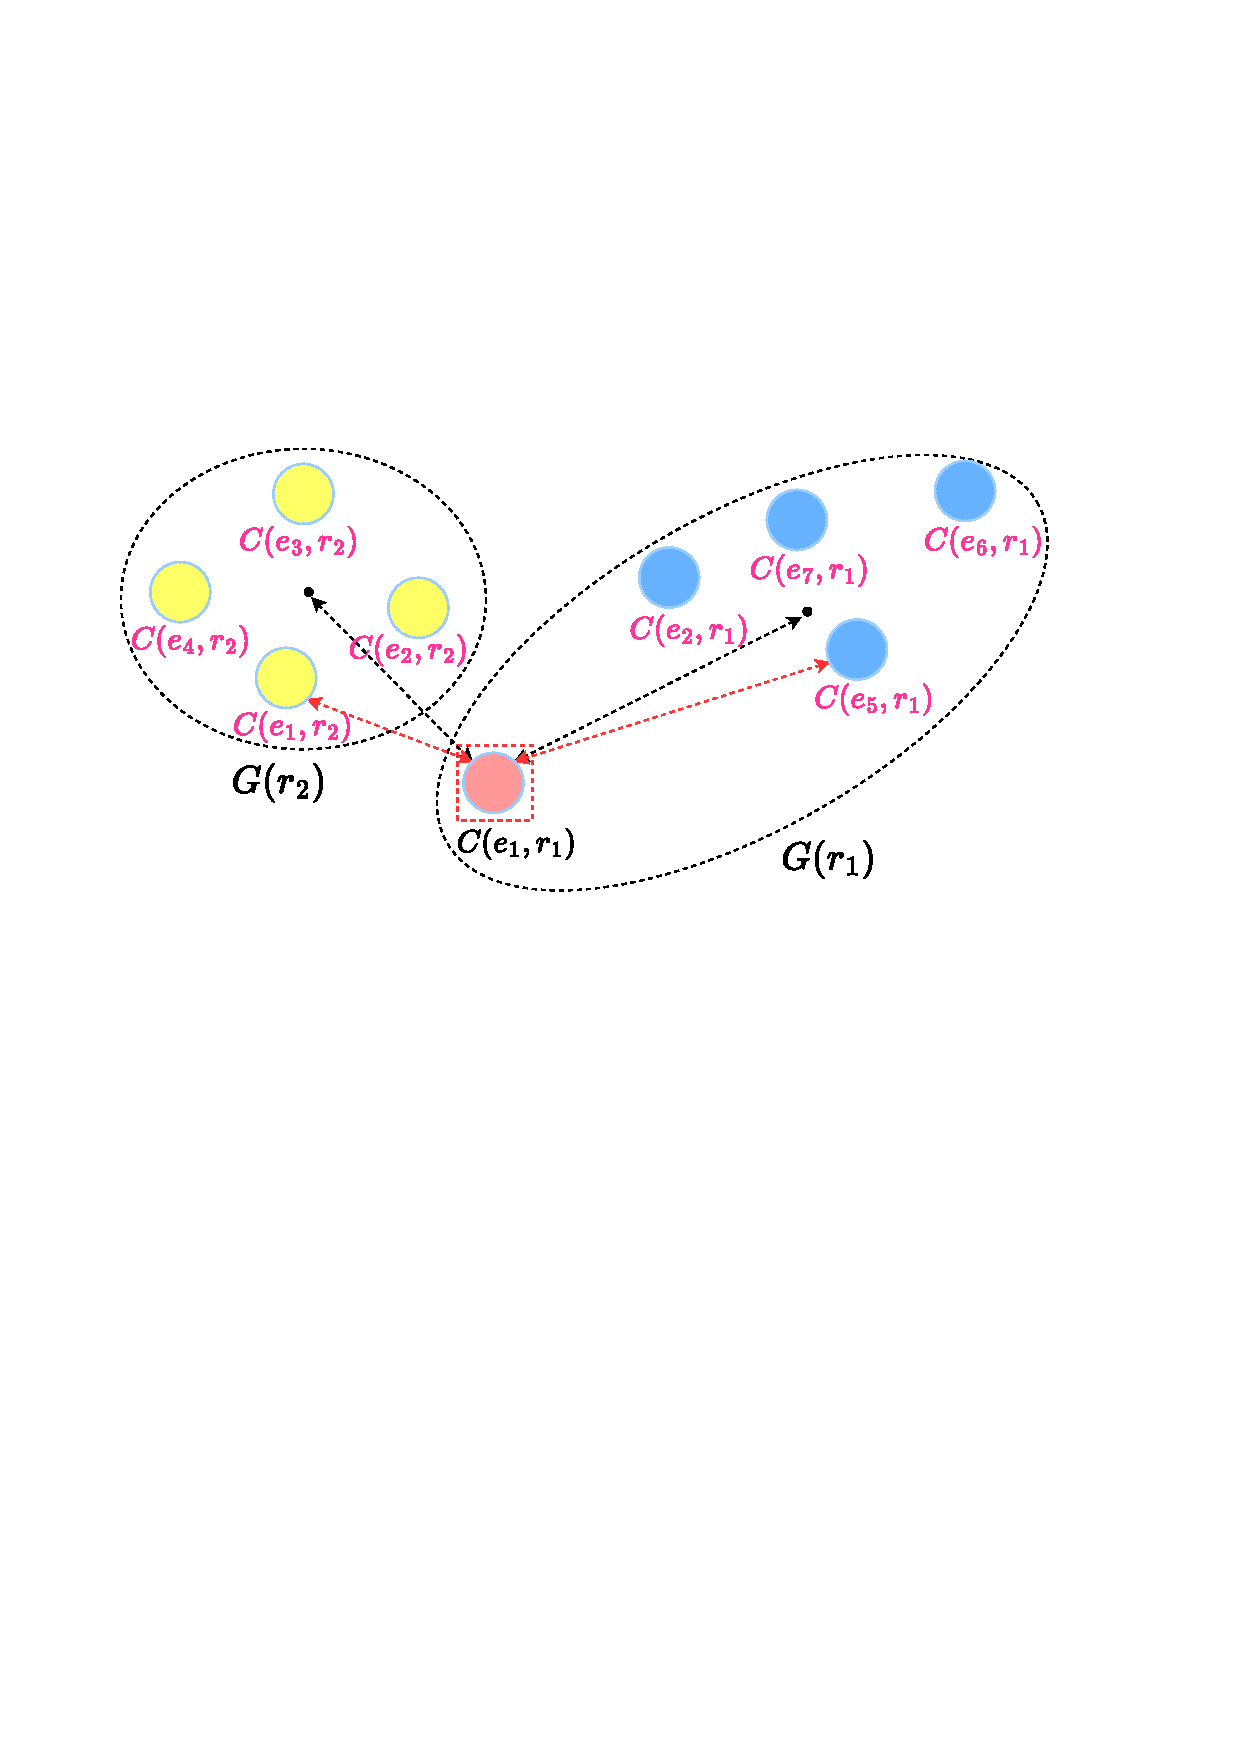
\includegraphics[width=0.7\linewidth]{figures/chap4/overdependence.pdf}
   \caption{实体类型过度依赖示例图}
   \label{fig-overdependence}
\end{figure}

\subsection{预实验验证}
\label{pre_experiment}
基于实体类型过度依赖的定义,本章节通过预实验验证其对于事件要素抽取性能的影响。

\textbf{数据集和模型}~在数据集方面,预实验评估选择了广泛使用的事件检测语料库ACE2005数据集,其具体细节将在主实验章节进行阐述。在模型方面,由于RNN、CNN和BERT是事件要素抽取最常用的三类编码器,预实验基于所选数据集训练了三种不同的事件要素抽取模型,包括AttRNN、DMCNN~\cite{chen2015event}和DMBERT~\cite{wang2019adversarial}。其中,基于RNN的事件要素抽取模型如JRNN~\cite{nguyen2016joint}和dbRNN~\cite{sha2018jointly}未公布源代码,因此本文受Lu等人~\cite{lu2019distilling}研究工作的启发,利用增加了注意力机制的双向LSTM作为使用RNN架构的基线模型,记作AttRNN。此外,由于训练集和测试集之间的数据分布相似,实验中将根据实体类型依赖、语义不一致和实体类型过度依赖的定义,分别评估测试集中相应簇的性能。由于事件要素抽取的测试集依赖于事件检测的预测结果,本文遵循Wang等人和Xi等人~\cite{wang2019hmeae,xiangyu2021capturing}的实验设置,分别使用训练好的AttRNN、DMCNN和DMBERT来检测事件类型和相应的触发词。考虑到测试的实例数量取决于不同事件检测模型正确预测的事件数量,本实验中三种基线模型对应的测试集实例数分别为4013、3630和4081。

\textbf{实验步骤}~首先,对于给定模型,本章使用其编码器获取测试集中每个实例的特征编码表示。然后,基于要素类型,测试集中的所有实例被划分为不同的群组,使得每个群组中实例的要素类型是相同的。进一步地,根据实体类型,将每个群组中的实例划分为不同的簇。因此,同一簇中实例的实体类型和要素类型是相同的。对于AttRNN、DMCNN和DMBERT各自对应的编码器,根据上述划分步骤可分别得到簇的数目为156、148和161。基于此,本章通过简单地计算各个群组/簇中所有实例特征表示的平均值,以用作其整体表示,其避免了引入额外计算参数和降低了计算复杂度。然后,本实验根据实体类型依赖、语义不一致和实体类型过度依赖的定义对每个簇进行判定,并分别计算符合不同定义的测试子集的性能(F1值)。

\textbf{评估验证}~预实验结果如表\ref{performance_pre}所示,其展示了根据不同定义类型划分的测试子集的簇数目及相应性能结果。从表中可以观察到:(1)对于不同的事件要素抽取模型,符合实体类型过度依赖的实例簇的性能都较低。其与其他类型的实例簇之间的巨大性能差异表明,现有事件要素抽取基线模型不擅长处理实体类型过度依赖问题。(2)符合实体类型过度依赖的实例簇和语义不一致的实例簇之间的性能差异表明,与语义不一致相比,由实体类型和要素类型之间的相关性导致的实体类型过度依赖进一步降低了模型的性能。(3)未对实体类型信息过度依赖的簇和整个测试集的性能差异表明,如果事件要素抽取模型缓解了实体类型过度依赖问题,则整体性能可以得到提升。

\begin{table*}[htp]
\footnotesize
\centering
\caption{测试集中不同类型实例簇的数目及性能结果}
\label{performance_pre}
\begin{tabular}{l|ccccc}
\toprule
模型  & \begin{tabular}[c]{@{}c@{}}实体类型依赖\\ (数目/F1 (\%))\end{tabular} & \begin{tabular}[c]{@{}c@{}}语义不一致\\ (数目/F1 (\%))\end{tabular} & \begin{tabular}[c]{@{}c@{}}实体类型过度依赖\\ (数目/F1 (\%))\end{tabular} & \begin{tabular}[c]{@{}c@{}}非实体类型过度依赖\\ (数目/F1 (\%))\end{tabular} & \begin{tabular}[c]{@{}c@{}}所有簇\\ (数目/F1 (\%))\end{tabular} \\ \midrule
AttRNN  & 100 / 40.6  & 56 / 38.9 & 48 / \textbf{18.1} & 108 / 63.6  & 156 / 50.9    \\
DMCNN   & 112 / 46.0 & 76 / 32.6 & 52 / \textbf{15.6} & 96 / 71.4  & 148 / 53.5    \\
DMBERT  & 95 / 38.6 & 48 / 40.7 & 31 / \textbf{15.3} & 130 / 68.9  & 161 / 57.2   \\ \bottomrule
\end{tabular}
\end{table*}

由于不同簇中的实例数量差异较大,本章节进一步统计了符合实体类型过度依赖的簇中实例的数目占据所有测试实例的比例,记作“实体类型过度依赖比例”。表\ref{number_pre}展示了不同事件要素抽取模型的比例结果。本文将在章节\ref{evaluation_section}中评估下一节所提的实体类型过度依赖消解方法是否可以降低“实体类型过度依赖比例”,进而提高整体性能。

\begin{table*}[htp]
\centering
\small
% \setlength{\abovecaptionskip}{0pt}
% \setlength{\belowcaptionskip}{10pt}
\caption{符合实体类型过度依赖的簇中实例统计信息}
\label{number_pre}
\begin{tabular}{l|ccc}
\toprule
模型 & 实体类型过度依赖的簇中实例数 & 总实例数 & 实体类型过度依赖比例(\%) \\ \midrule
AttRNN  & 2845  & 4013  & 70.9  \\
DMCNN   & 2799  & 3630  & 77.1  \\
DMBERT  & 1281  & 4081  & 31.4  \\ \bottomrule
\end{tabular}
\end{table*}

从预实验中可以观察到,实体类型过度依赖问题降低了事件要素抽取模型的整体性能。为了缓解该问题,本文考虑降低“实体类型过度依赖比例”。进一步,其是由实体类型依赖导致,则可以利用以下两种方式处理:(1)增加具有相同要素类型但实体类型不同的实例特征表示之间的相似性;(2)降低具有不同要素类型但实体类型相同的实例特征表示之间的相似性。基于此,下一节将具体介绍将上述两种方式整合的所提方法,从而提高事件要素抽取的性能。

\section{方法设计}
本章将详细介绍基于多角度对比学习的实体类型过度依赖消解方法,其可以应用于不同的事件要素抽取基线模型。为了描述方便,本章选取DMBERT~\cite{wang2019adversarial},以其为基础介绍相应的多角度实体类型过度依赖消解的事件要素抽取模型METOR。图\ref{framework}展示了所提模型的总体架构,其主要由四个模块组成:编码器、正样本处理、负样本处理和循环训练策略。

\begin{figure}[htp]
    \centering
   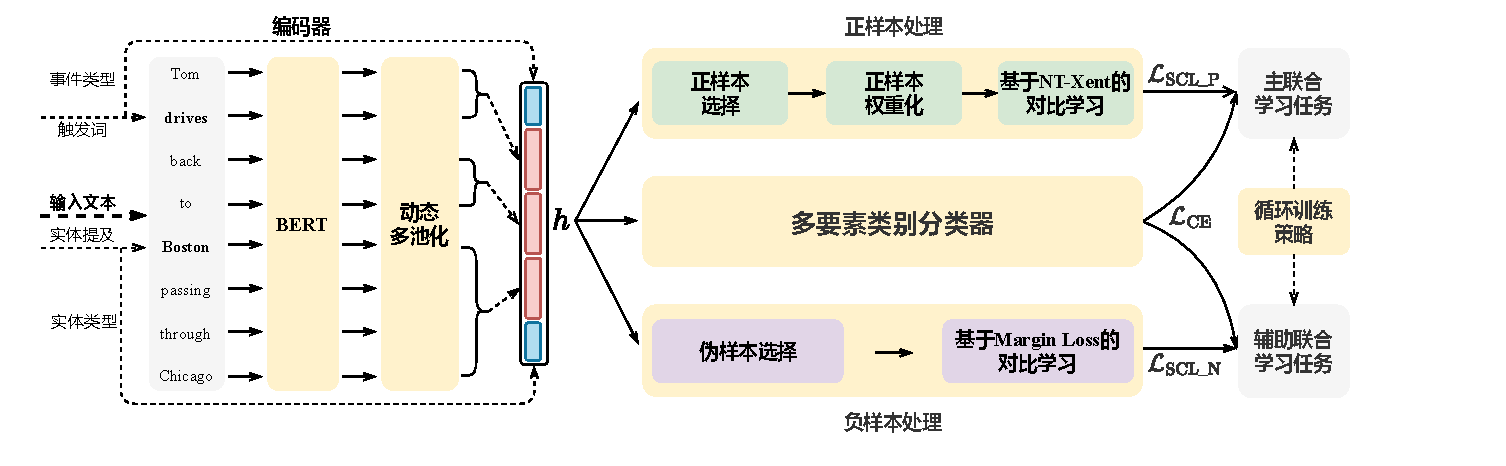
\includegraphics[width=1\linewidth]{figures/chap4/framework_metor.pdf}
   \caption{METOR模型架构图}
   \label{framework}
\end{figure}

\subsection{编码器}
编码器模块旨在将每个实例编码成对应的特征表示。由于事件要素抽取为事件检测的后续任务,本章节遵循Wang等人~\cite{wang2019hmeae}和Xi等人~\cite{xiangyu2021capturing}的研究工作,先利用Wang等人~\cite{wang2019hmeae}提出的DMBERT事件检测模型进行事件触发词和相应事件类型的预测,并将所有实体提及设置为待抽取的事件要素候选。由于句子中可能存在多个事件要素候选,本章将这些候选分成多个实例处理。假设给定的事件要素候选为$arg$,其实体类型为$e$,所参与预测的事件触发词为
$tri$,对应的事件类型为$t$,首先利用BERT~\cite{devlin2019bert}对所在句子文本$x=\left\{w_{1},\cdots,tri,\cdots ,arg, \cdots, w_{n}\right\}$进行编码得到特征表示:
\begin{equation}
  \left\{\boldsymbol{\hat{h}}_{1},\cdots,\boldsymbol{\hat{h}}_{p_{tri}},\cdots,\boldsymbol{\hat{h}}_{p_{arg}},\cdots,\boldsymbol{\hat{h}}_{n}\right\}=\textrm{BERT}(w_{1},\cdots, tri,\cdots, arg, \cdots, w_{n})
\end{equation}
其中$p_{tri}$和$p_{arg}$分别表示$tri$和$arg$在输入句子中的位置。

在此之后,使用一个动态多池化操作分段聚合编码后的特征表示:
\begin{equation}
    \left[\boldsymbol{h}_{1, p_{tri}}\right]_{k}=\max \left\{\left[\boldsymbol{\hat{h}}_{1}\right]_{k} \cdots,\left[\boldsymbol{\hat{{h}}}_{p_{tri}}\right]_{k}\right\}
\end{equation}
\begin{equation}
    \left[\boldsymbol{{h}}_{p_{tri}+1, p_{arg}}\right]_{k}=\max \left\{\left[\boldsymbol{\hat{h}}_{p_{tri}+1}\right]_{k} \cdots,\left[\boldsymbol{\hat{{h}}}_{p_{arg}}\right]_{k}\right\}
\end{equation}
\begin{equation}
    \left[\boldsymbol{{h}}_{p_{arg}+1, n}\right]_{k}=\max \left\{\left[\boldsymbol{\hat{h}}_{p_{arg}+1}\right]_{k} \cdots,\left[\boldsymbol{\hat{{h}}}_{n}\right]_{k}\right\}
\end{equation}
其中$[\cdot]_{k}$表示对应向量的第$k$个值。然后,本章随机初始化所有的事件类型标签和实体类型标签,分别表示为$\boldsymbol{W}_{T} \in {\mathbb{R}}^{n_{t} \times d_{s}}$和$\boldsymbol{W}_{E} \in {\mathbb{R}}^{n_{e} \times d_{s}}$。其中,$d_{s}$、$n_{t}$和$n_{e}$分别表示事件类型(实体类型)向量的维度、预定义的事件类型数目和预定义的实体类型数目。此外,$\boldsymbol{W}_{T}\left(t\right)$表示使用
事件类型$t$从向量矩阵$\boldsymbol{W}_{T}$中查找出的事件类型向量。类似地,$\boldsymbol{W}_{E}\left(e\right)$表示根据实体类型$e$查找出的实体类型向量。最后,串接上述表示,得到实例的特征表示$\boldsymbol{h} \in {\mathbb{R}}^{d_{out}}$如下:
\begin{equation}
\label{input_information}
\boldsymbol{h}=\left[\boldsymbol{h}_{1, p_{tri}};\boldsymbol{{h}}_{p_{tri}+1, p_{arg}};\boldsymbol{{h}}_{p_{arg}+1, n};\boldsymbol{W}_{T}\left(t\right);\boldsymbol{W}_{E}\left(e\right)\right]
\end{equation}

\subsection{正样本处理}
本模块提出了一种选择-加权的对比学习方法,该方法包括三个步骤:正样本选择、正样本加权和基于归一化温度标度交叉熵(NT-Xent)的对比学习。首先,该方法基于给定实例的实体类型选择正样本,使得模型能够聚焦于处理与给定实例的实体类型无关的正样本。然后,计算全局共现信息和语义相关性信息,以对所选正样本的相关性进一步权重化处理。基于此,模型可以提升特定正样本的对比学习贡献,其包含了更多与给定实例要素类型相关的关键语义信息,从而学习到实体类型信息之外的更多有效语义知识。最后,计算基于NT-Xent的选择-加权对比学习方法的训练损失。

\textbf{正样本选择}~给定一批包含$K$个实例的批数据 $\mathcal{B}$,对于其中的每个实例$x_{i}$,首先选择与其要素类型相同的实例作为正样本集合$\mathcal{P}\left(x_{i}\right)$,选择与其要素类型不同的实例作为负样本集合$\mathcal{N}\left(x_{i}\right)$。基于
$\mathcal{P}\left(x_{i}\right)$,本节采用一个简单的选择策略去获取新的正样本集合:
\begin{equation}
  \mathcal{P}_{s}\left(x_{i}\right)=\left\{x_{p}: x_{p} \in \mathcal{B}, (e_{p} \neq e_{i}) \wedge (r_{p}=r_{i}) \wedge (p \neq i)\right\}
\end{equation}
其中$r_{i}$和$e_{i}$分别表示实例$x_{i}$的要素类型和实体类型。本选择策略只用于包含了不止一个样本的$\mathcal{P}\left(x_{i}\right)$,以避免造成对比数据的稀疏。

\textbf{正样本加权}~在完成正样本选择后,本章根据要素类型$r_{i}$,对$\mathcal{P}_{s}\left(x_{i}\right)$中的每个正样本分配一个权重。传统的对比学习方法在对比学习损失中等同地对待所有正样本,无法区分具有不同实体类型的正样本的重要程度。为此,本章基于要素类型$r_{i}$,从全局共现信息和语义相关性信息两个方面,计算不同正样本对于$x_{i}$的重要性。

全局共现信息可表示为记录了整个训练集中不同实体类型和要素类型共现数量的共现矩阵$I_{e,r}$。假设$\mathcal{E}$和$\mathcal{R}$分别为训练集中的实体类型和要素类型集合,批数据$\mathcal{B}$中第$p$个实例(即$x_{p}$)存在于集合$\mathcal{P}_{s}\left(x_{i}\right)$中,其实体类型为$e_{p}$。受TF-IDF~\cite{salton1988term}启发,首先定义实体类型频率(ETF),用于表示$e_{p}$与$r_{i}$同时出现的频率:
\begin{equation}
  {\textrm{ETF}}\left(e_{p}, r_{i}\right)=\frac{I_{e_{p},r_{i}}}{\sum_{m \in \mathcal{E}} I_{m,r_{i}}}
\end{equation}

此外,本章使用与$e_{p}$同时出现的要素类型的数量来衡量$e_{p}$的重要性。要素类型数量越少,$e_{p}$则越重要。因此,反向要素类型频率(IRTF)可根据如下定义得到:
\begin{equation}
  {\textrm{IRTF}}\left(e_{p}\right)=\log \frac{|\mathcal{R}|}{|\{r \in \mathcal{R}: I_{e_{p},r} > 0\}|+1}
\end{equation}

基于ETF和IRTF,可得实例$x_{p}$对于实例$x_{i}$在全局共现信息方面的重要性得分:
\begin{equation}
 w_{1}\left(x_{p}, x_{i}\right)= {\textrm{ETF}}\left(e_{p}, r_{i}\right) \times {\textrm{IRTF}}\left(e_{p}\right)
\end{equation}

然而,在事件类型不同的实例中,具有相同实体类型的实体提及可能以不同的要素类型参与在事件中。因此,对于不同的事件类型,即使实例的实体类型相同,对给定实例的重要性也应有所区分。因此,考虑$x_{p}$对$x_{i}$的重要性时仅使用全局共现信息不足以建模不同事件类型的影响。基于此,本节进一步利用语义相关性信息。首先,将所有要素类型标签随机初始化成向量矩阵$\boldsymbol{W}_{R} \in {\mathbb{R}}^{n_{r} \times d_{s}}$,其中$n_{r}$为预定义的要素类型的数目(包括特殊要素类型“空”),$d_s$是要素类型向量的维度。然后,对于给定的实例$x_{i}$,得到融合事件类型信息的实体类型和要素类型表示:
\begin{equation}
 \boldsymbol{e}_{i}^{t} = \boldsymbol{W}_{T}\left(t_{i}\right) \odot \boldsymbol{W}_{E}\left(e_{i}\right)
 \label{eq9}
\end{equation}
\begin{equation}
 \boldsymbol{r}_{i}^{t} = \boldsymbol{W}_{T}\left(t_{i}\right) \odot \boldsymbol{W}_{R}\left(r_{i}\right)
 \label{eq11}
\end{equation}
其中$\odot$表示元素依次相乘,$r_{i}$、$e_{i}$和$t_{i}$分别表示实例$x_{i}$的要素类型、实体类型和事件类型。$\boldsymbol{W}_{T}\left(t_{i}\right)$表示使用
事件类型$t_{i}$从向量矩阵$\boldsymbol{W}_{T}$中查找出的事件类型向量。类似地,可以分别得到实体类型向量$\boldsymbol{W}_{E}\left(e_{i}\right)$和要素类型向量$\boldsymbol{W}_{R}\left(r_{i}\right)$的含义。由于
$\boldsymbol{W}_{T}$和$\boldsymbol{W}_{E}$同时也是公式\ref{input_information}中串接向量的一部分,事件类型和实体类型的语义信息实现了在不同模块间的共享。同样,可以得到任意正样本$x_{p}$的融合事件类型信息的实体类型表示$\boldsymbol{e}_{p}^{t}$。然后,本章基于语义相关性信息,利用注意力机制计算$x_{p}$对于$x_{i}$的重要性得分,并根据$\textrm{softmax}$函数得到归一化结果$w_{2}\left(x_{p}, x_{i}\right)$:
\begin{equation}
s\left(x_{p},x_{i}\right)=\boldsymbol{v}^{\top} \tanh \left(\boldsymbol{U}\left[\boldsymbol{e}_{i}^{t};\boldsymbol{e}_{p}^{t};\boldsymbol{r}_{i}^{t}\right]\right)
\end{equation}
\begin{equation}
 w_{2}\left(x_{p}, x_{i}\right) =  \frac{\exp \left(s\left(x_{p},x_{i}\right)\right)}{\sum_{e_{j} \in \mathcal{E}}\exp \left(s\left(x_{j},x_{i}\right)\right)}
\end{equation}
其中$\boldsymbol{v} \in {\mathbb{R}}^{3d_{s}}$和$\boldsymbol{U} \in {\mathbb{R}}^{3d_{s} \times 3d_{s}}$分别表示可训练学习的向量和矩阵参数。然后,可得$x_{p}$对于$x_{i}$的最终重要性得分:
\begin{equation}
 {\textrm{w}}\left(x_{p}, x_{i}\right) = \alpha w_{1}\left(x_{p}, x_{i}\right) + (1-\alpha) w_{2}\left(x_{p}, x_{i}\right)
\end{equation}
其中$\alpha\,(0 < \alpha < 1)$为权重参数。

\textbf{基于NT-Xent的对比学习}~遵循Chen等人~\cite{chen2020simple}和Khosla等人~\cite{khosla2020supervised}的研究,本章首先将实例$x_{i}$的特征表示$\boldsymbol{h}_{i}$映射到一个新空间上,以提高对比学习的质量:
\begin{equation}
\label{map}
  \boldsymbol{z}_{i}=\boldsymbol{W}_{1} f\left(\boldsymbol{W}_{2} \boldsymbol{h}_{i}\right)
\end{equation}
$\boldsymbol{W}_{1} \in {\mathbb{R}}^{d_{1} \times d_{2}}$和$\boldsymbol{W}_{2} \in {\mathbb{R}}^{d_{2} \times d_{out}}$为可训练学习的矩阵参数,$f(\cdot)$为ReLU激活函数,其中$d_{1}$和 $d_{2}$为维度参数。在选择出正样本并对其权重化后,本章基于NT-Xent~\cite{chen2020simple}计算相应的对比学习损失$\mathcal{L_\textrm{SCL\_P}}$如下:
\begin{equation}
\label{nt_loss}
\mathcal{L_\textrm{SCL\_P}}=\sum_{i=1}^{K} \frac{-1}{|\mathcal{P}_{s}\left(x_{i}\right)|} \sum_{p \in \mathcal{P}_{s}\left(x_{i}\right)} {\textrm{w}}(x_{p}, x_{i}) \cdot \log \frac{\exp \left(\textrm{sim}\left(\boldsymbol{z}_{i},\boldsymbol{z}_{p}\right) / \tau\right)}{\sum_{n \in K\backslash i }\exp \left(\textrm{sim}\left(\boldsymbol{z}_{i},\boldsymbol{z}_{n}\right) / \tau\right)}
\end{equation}
其中$\textrm{sim}\left(\boldsymbol{z}_{i},\boldsymbol{z}_{p}\right)=\boldsymbol{z}_{i}^\top\boldsymbol{z}_{p}/\lVert\boldsymbol{z}_{i}\rVert \,\lVert\boldsymbol{z}_{p}\rVert$,$\tau$表示温度参数。

\subsection{负样本处理}
本模块提出了一种伪正对比学习方法,该方法包括两个步骤:伪样本选择和基于边际损失(Margin Loss)的对比学习。首先,基于实体类型从负样本中选择出伪正样本。然后,利用这些选择出的样本作为对比参考,降低给定实例和与其实体类型相同的负样本之间的特征表示相似性。

\textbf{伪样本选择}~给定一批包含$K$个实例的批数据$\mathcal{B}$,对于其中的每个实例$x_{i}$,首先选择对应的伪正样本和伪负样本,选择过程如下:
\begin{equation}
  \mathcal{P}_{pseudo}\left(x_{i}\right)=\left\{x_{p}: x_{p} \in \mathcal{B}, (e_{p} \neq e_{i}) \wedge (r_{p} \neq r_{i}) \wedge (p \neq i)\right\}
\end{equation}
\begin{equation}
  \mathcal{N}_{pseudo}\left(x_{i}\right)=\left\{x_{n}: x_{n} \in \mathcal{B}, (e_{n}=e_{i}) \wedge (r_{n} \neq r_{i}) \wedge (n \neq i)\right\}
\end{equation}
其中伪正样本集合和伪负样本集合分别表示为 $\mathcal{P}_{pseudo}\left(x_{i}\right)$和 $\mathcal{N}_{pseudo}\left(x_{i}\right)$。

\textbf{基于边际损失的对比学习}~
首先,本章计算$\mathcal{P}_{pseudo}\left(x_{i}\right)$和 $\mathcal{N}_{pseudo}\left(x_{i}\right)$中实例特征表示的平均值,分别得到$\boldsymbol{z}_{i}^{P}$和$\boldsymbol{z}_{i}^{N}$,以表示这两个集合的整体信息。然后,利用$\mathcal{P}_{pseudo}\left(x_{i}\right)$作为对比参考进行对比学习,以降低实例$x_{i}$与属于$\mathcal{N}_{pseudo}\left(x_{i}\right)$的样本之间的相似性。由于$\mathcal{P}_{pseudo}\left(x_{i}\right)$中的样本本质上仍是$x_{i}$的负样本,使用实例级的对比学习损失NT-Xent以增加伪正样本与给定实例之间的相似性是不合适的。因此,本章使用边际损失来对伪正样本集合和伪负样本集合的整体表示进行对比学习:
\begin{equation}
\label{eq21}
  \mathcal{L_\textrm{SCL\_N}} =\sum_{i=1}^{K} \max \left\{\boldsymbol{z}_{i}^{N} \cdot \boldsymbol{z}_{i}-\boldsymbol{z}_{i}^{P} \cdot \boldsymbol{z}_{i}+\gamma, 0\right\}
\end{equation}
其中$\gamma$为边际超参数。

\subsection{循环训练策略}
本模块首先计算事件要素抽取任务的损失。给定实例$x$,将其从编码器模块得到的特征表示\boldsymbol{$h$}输入到多要素类别分类器,以计算概率分布$p\left(x\right)$如下:
\begin{equation}
  p\left(x\right) = \textrm{softmax}\left(\boldsymbol{W}^{c}\boldsymbol{h} + \boldsymbol{b}^{c}\right)
 \label{eq3}
\end{equation}
其中$\boldsymbol{W}^{c} \in {\mathbb{R}}^{n_{r} \times d_{out}}$和$\boldsymbol{b}^{c} \in {\mathbb{R}}^{n_{r}}$分别表示分类器中要训练的参数。给定包含$K$个实例的批数据$\mathcal{B}$,交叉熵损失$\mathcal{L_\textrm{CE}}$计算如下:
\begin{equation}
  \mathcal{L_\textrm{CE}} = -\sum^{K} \log p\left(r|x\right)
 \label{ce}
\end{equation}
其中$p\left(r|x\right)$表示将实例$x$预测为正确的要素类型$r$的概率值。在测试阶段,$p\left(x\right)$用于获取事件要素抽取的预测要素类型。

进一步,本章注意到优化$\mathcal{L_\textrm{SCL\_N}}$将不可避免地提升实例$x_{i}$和$\mathcal{P}_{pseudo}\left(x_{i}\right)$中的样本(本质上为负样本)间的特征表示相似度。然而,根据公式\ref{nt_loss},优化$\mathcal{L_\textrm{SCL\_P}}$会降低实例$x_{i}$和所有负样本间的特征表示相似度。因此, $\mathcal{L_\textrm{SCL\_N}}$和$\mathcal{L_\textrm{SCL\_P}}$的训练目标是不一致的。为此,本章提出了一个循环训练策略,该策略依次使用两个不同的联合训练目标来协调$\mathcal{L_\textrm{SCL\_P}}$和 $\mathcal{L_\textrm{SCL\_N}}$的不一致。具体来说,将联合优化$\mathcal{L_\textrm{SCL\_P}}$和 $\mathcal{L_\textrm{CE}}$视作主联合学习任务,先训练$f$轮,其中$f$是超参数。然后,将联合优化$\mathcal{L_\textrm{SCL\_N}}$和 $\mathcal{L_\textrm{CE}}$视作辅助联合学习任务,再训练一轮。重复上述过程直到训练完成。通过这种方式,可以逐步调整处理$\mathcal{L_\textrm{SCL\_P}}$和$\mathcal{L_\textrm{SCL\_N}}$训练目标的不一致。本章提出的训练策略表示如下:
\begin{equation}
\label{eq24}
\mathcal{L_\textrm{JOINT}}=\left\{\begin{array}{lr}
 \mathcal{L_\textrm{SCL\_P}}+\mathcal{L_\textrm{CE}} & epoch \bmod f \neq 0 \\
 \mathcal{L_\textrm{SCL\_N}}+\mathcal{L_\textrm{CE}} & epoch \bmod f = 0 
\end{array}\right.
\end{equation}
其中$epoch$表示完成训练的轮次。

\section{实验评估}
\label{evaluation_section}
在实验评估中,本章所提的方法不仅应用于基线模型DMBERT,也应用于AttRNN和DMCNN基线模型,分别记作METOR(RNN)和METOR(CNN)。在METOR(RNN)和METOR(CNN)中,将编码器模块中的DMBERT分别替换为AttRNN和DMCNN,其他模块保持不变。由于事件要素抽取任务依赖于事件检测的结果,本章遵循Wang等人~\cite{wang2019hmeae}和Xi等人~\cite{xiangyu2021capturing}的研究设定,使用经过训练的AttRNN、DMCNN和DMBERT分别检测事件触发词和相应的事件类型,作为METOR(RNN)、METOR(CNN)和METOR模型的输入。接下来,本章将介绍实验设置、性能结果、消融研究、实体类型信息深入分析、超参数敏感性分析、计算复杂性分析和案例研究。

\subsection{实验设置}
\label{settings_4}
\textbf{1.数据集}~遵循最近主流的给定实体提及的事件要素抽取研究工作~\cite{xiangyu2021capturing,liu2018jointly, nguyen2016joint},本章实验评估在ACE2005数据集上进行。与章节\ref{experiment_settings}相同,其为ACE2005语料库~\cite{doddington2004automatic}中的英文版本数据集。根据Wang等人~\cite{wang2019hmeae}的预处理设置\footnote{https://github.com/thunlp/HMEAE},该数据集包含599个文档、33种事件类型、46种实体类型和35种事件要素类型。此外,引入$None$(空)作为特殊要素类型,以表示相应的候选要素在给定实例中为非事件要素。进一步,该数据集被划分为529、30和40个文档,分别作为训练集、验证集和测试集。

\textbf{2.评价指标}~本章实验遵循事件要素抽取任务的标准评估。如果事件类型、偏移量和要素类型与数据集的标注完全相同,则认定候选要素被正确抽取,其中偏移量指候选要素文段在句子中的开始和结束位置索引。基于此,本文使用准确率(P)、召回率(R)和F1值(F1)作为评估指标,其计算方式参照章节\ref{experiment_settings}。

\textbf{3.实验配置}~在编码器模块中,对于METOR(RNN)本章使用预训练Glove词向量、随机初始化事件类型向量、随机初始化实体类型向量和随机初始化位置向量,维度分别为100、5、5和5,并在模型中使用双向LSTM和自注意力机制。对于METOR(CNN),使用与DMCNN相同的输入向量和超参数。类似地,本章将5维随机初始化的实体类型向量添加到METOR(CNN)的输入中。对于METOR,编码使用的BERT预训练模型为HuggingFace发布的“google-bert/bert-base-uncased”版本\footnote{https://huggingface.co/google-bert/bert-base-uncased},实体类型向量维度$d_{s}$设置为50。在正样本处理模块中,本章将$d_{1}$设置为512,$d_{2}$设置为512,温度参数$\tau$设置为0.1,权重$\alpha$设置为0.7。在负样本处理模块中,将$\gamma$设置为0.1。在循环训练策略中,METOR(RNN)、METOR(CNN)和METOR的循环频率$f$分别设置为4、3和3。此外,其批数据大小均设置为80,训练轮次设置为10,优化器使用AdamW,对应的学习率分别设置为$1 \times 10^{-3}$, $1 \times 10^{-3}$和$5 \times 10^{-5}$。对于不同的模型,训练均在相同实验服务器上进行,具体配置为:CPU型号Intel(R) Xeon(R) Gold 5320,主频2.20GHz;内存256G;GPU计算卡型号NVIDIA GeForce RTX 3090,显存24G。上述模型均基于Pytorch~\cite{paszke2017automatic}框架进行构建。

\textbf{4.基线模型}~本节选择以下模型作为实验比较的基线:

\begin{itemize}
\item DMCNN \cite{chen2015event} - 该模型使用了CNN和动态多池化操作提取实例的特征表示。
\item JRNN \cite{nguyen2016joint} - 该模型提出了包含离散二元矩阵的RNN,其利用了事件类型和要素类型、要素类型间的相互依赖性。
\item dbRNN \cite{sha2018jointly} - 该模型在RNN中引入了依存句法信息,并构建事件内候选要素间的交互向量以捕捉其关联性。
\item DMBERT \cite{wang2019adversarial} - 该模型使用了BERT和动态多池化操作来提取实例的特征表示。
\item PLMETOR \cite{yang2019exploring} - 该模型基于BERT来预测事件要素类型并生成额外的训练实例,以进一步提高性能。
\item HMEAE \cite{wang2019hmeae} - 该模型提出了一种利用事件要素类型语义相关性的层次模块化注意力网络。
\item BERT (Inter) \cite{xiangyu2021capturing} - 该模型基于BERT并利用了跨事件的相互依赖关系
~\cite{nguyen2016joint}。
\item BERT (Intra) \cite{xiangyu2021capturing} - 该模型基于BERT并利用了事件内部的要素依赖关联~\cite{sha2018jointly}。 
\item BERD \cite{xiangyu2021capturing} - 该模型提出了一种能够利用事件内其他要素的类型预测语义信息的的编码器-解码器框架。
\end{itemize}

本章注意到RCEE\_ER~\cite{liu2020event}在F1指标上取了优秀的性能表现,但其受益于额外的数据增广和无监督数据。因此,本章遵循Xi等人~\cite{xiangyu2021capturing}在BERD模型中的基线模型设置,未将RCEE\_ER模型作为实验性能比较的基线。此外,本章将ChatGPT在ACE2005数据集上的性能评估保留到章节\ref{section_5_3}进行展示与分析。

\subsection{性能结果}

表\ref{overall_4_4}展示了本章所提方法与基线模型在ACE2005数据集上的性能结果,其中$\dagger$表示将本章提出的方法应用在DMBERT基线模型时,其性能在双侧$t$检验下显著($p < 0.01$)优于之前性能最优的事件要素抽取模型BERD。根据结果可进一步观察到,与AttRNN相比,METOR(RNN)在F1指标上实现了3.9\%的性能提升。即使与利用了事件类型和要素类型、要素类型间的相互依赖性的JRNN相比,METOR(RNN)也取得了相差无几的F1指标结果。此外,dbRNN的F1指标显著优于METOR(RNN),本文将其归因于两个原因:(1)dbRNN利用了额外的句法信息。(2)dbRNN同时优化了事件检测和事件要素抽取任务的性能,而METOR(RNN)没有受益于这种联合优化。当本章提出的方法应用在DMCNN时,METOR(CNN)相比该基线在F1指标上实现了5\%的提升,比同样使用了DMCNN作为编码器的HMEAE(CNN)提升了2.8\%。并且,METOR(CNN)的F1指标优于大多数没有使用预训练模型的事件要素抽取模型,并与dbRNN相比时展现了相当的性能结果。同时,可以观察到METOR(CNN)的性能优于使用了BERT预训练模型作为编码器的DMBERT、PLMETOR和BERT(Inter)。

当在编码器模块使用DMBERT时,METOR取得了当前最优的F1性能
% {我们注意到,2020年提出的在F1评分中达到了63.6\%。然而,RCEE得益于额外的资源,包括数据论证和无监督数据。因此,我们遵循BERD于2021年提出的模型,并且不将我们提出的模型与RCEE模型进行比较,因为两者在使用外部资源方面存在差异。)(在F1中)
,且相比于之前性能最优的BERD模型提升了2.1\%。此外,METOR的F1指标比相应的DMBERT基线高出了5.2\%。总的来说,由于本章所提的METOR模型可以学习到除实体类型之外的更多语义信息,从而消解了实体类型过度依赖问题,实现了在事件要素抽取任务上对所有基线模型的性能超越。

\begin{table}[htp]
\centering
% \small
% \setlength{\abovecaptionskip}{0pt}
% \setlength{\belowcaptionskip}{10pt}
\caption{ACE2005数据集上的事件要素抽取性能结果}
% $\textrm{METOR}_{avg}$ is the average performance of METOR and $\pm$ represents the standard deviation when five different random seeds are used. 
% $\dagger$ denotes that our model significantly outperforms the best baseline BERD with $p < 0.01$ under a paired two-sided t-test.}
\label{overall_4_4}
\begin{tabular}{lccc}
\toprule
\multicolumn{1}{l|}{模型}       & P(\%)                          & R(\%)                          & F1(\%)                         \\ \midrule
\multicolumn{1}{l|}{AttRNN}        & 50.6                           & 51.1                           & 50.9                         \\
\multicolumn{1}{l|}{DMCNN}        & 62.2                           & 46.9                           & 53.5                           \\
\multicolumn{1}{l|}{JRNN}         & 54.2                           & 56.7                           & 55.4                           \\
\multicolumn{1}{l|}{dbRNN}        & \textbf{66.2}                & 52.8                           & 58.7                           \\
\multicolumn{1}{l|}{HMEAE (CNN)}  & 57.3                           & 54.2                           & 55.7                           \\
\multicolumn{1}{l|}{\textbf{METOR (RNN)}}   & 51.9      &  58.0      &  54.8 \\
\multicolumn{1}{l|}{\textbf{METOR (CNN)}}   & 56.2      & 61.1     & 58.5  \\ \midrule
+ BERT ($base$)               &                                &                                &                                \\ \midrule
\multicolumn{1}{l|}{DMBERT}       & 58.8                           & 55.8                           & 57.2                           \\
\multicolumn{1}{l|}{PLMETOR}        & 62.3                           & 54.2                           & 58.0                           \\
\multicolumn{1}{l|}{BERT (Inter)} & 58.4                           & 57.1                           & 57.8                           \\
\multicolumn{1}{l|}{BERT (Intra)} & 56.4                           & 61.2                           & 58.7                           \\
\multicolumn{1}{l|}{HMEAE (BERT)} & 62.2                           & 56.6                           & 59.3                           \\
\multicolumn{1}{l|}{BERD}         & 59.1                           & 61.5                           & 60.3                           \\
\multicolumn{1}{l|}{\textbf{METOR}} & 60.3                           & $\boldsymbol{64.7}$          &$\boldsymbol{62.4^{\dagger}}$ \\
\bottomrule
% \multicolumn{1}{l|}{$\textbf{METOR}_{avg}$} & $60.14\pm1.16$                            & 64.36$\pm$0.60          &$62.14\pm0.56^{\dagger}$  \\
% \midrule
\end{tabular}
\end{table}

\subsection{消融研究}
本章通过消融研究分析所提方法中每个模块的有效性,包括正样本处理(Positive Sample Processing)、负样本处理(Negative Sample Processing)和循环训练策略(Cyclic Training Strategy),其中$\Delta$ F1表示与完整方法在F1指标上的性能差距。如表\ref{ablation}所示,将本章所提的方法应用到不同的基线模型上,三个模块都能提升相应基线模型的性能。本节选择METOR模型进行着重讨论。首先,如果移除正样本处理和负样本处理模块,METOR模型在F1指标上的性能将分别下降2.0\%和1.3\%,这表明从正样本和负样本角度消解实体类型过度依赖都可以有效地提升事件要素抽取性能。其次,如果将不同模块的损失直接求和并进行联合训练,以替代循环训练策略,则METOR模型在F1上的性能将下降2.9\%。这表明循环训练策略可以有效地调和正样本处理模块和负样本处理模块中的不同对比学习目标。此外,可以观察到即使移除掉正样本处理模块或负样本处理模块,METOR模型仍优于之前性能最优的BERD模型。本文将其归因于这两个模块都推动了模型学习除实体类型之外的更多语义信息,从而消解了实体类型过度依赖问题,提升了整体性能。

\begin{table*}[htp]
\centering
% \setlength{\abovecaptionskip}{0pt}
% \setlength{\belowcaptionskip}{10pt}
\caption{ACE2005数据集上的消融研究结果}
% $\Delta$ F1 is the performance difference in F1 when compared with the full model.}
\label{ablation}
\begin{tabular}{l|cccc}
\toprule
模型 & P(\%) & R(\%) & F1(\%) &$\Delta$ F1\\ 
\midrule
\textbf{METOR (RNN)} & 51.9      &  58.0      &  54.8  & -\\
w/o Positive Sample Processing & 48.7  & 55.7  & 52.0  & -2.8\\
w/o Negative Sample Processing & 51.1  & 57.2  & 54.0   & -0.8\\
w/o Cyclic Training Strategy & 50.8  & 52.7  & 51.7    & -3.1\\ 
\midrule
\textbf{METOR (CNN)} & 56.2      & 61.1      & 58.5  & -\\
w/o Positive Sample Processing & 52.9  & 59.2  & 55.9   & -2.6\\
w/o Negative Sample Processing & 57.4  & 56.3  & 56.8   & -1.7\\
w/o Cyclic Training Strategy & 54.0  & 57.4  & 55.7    & -2.8\\ 
\midrule
\textbf{METOR} & 60.3  & 64.7  & 62.4   & -\\
w/o Positive Sample Processing & 59.7      &  61.2     &  60.4      & -2.0\\
w/o Negative Sample Processing & 59.3  & 62.9  & 61.1   & -1.3\\ 
w/o Cyclic Training Strategy & 57.1  & 62.1  & 59.5   & -2.9\\  
\bottomrule
\end{tabular}
\end{table*} 

\subsection{实体类型信息分析}
作为基于实体的任务,实体类型信息对于事件要素抽取任务的影响是多方面的。一方面,实体类型是事件要素抽取任务中实体提及的主要信息来源。另一方面,其导致事件要素抽取模型产生了实体类型过度依赖,进而降低了模型的整体性能。因此,本节将对实体类型信息进行深入全面的分析。

\textbf{不同变体模型的实体类型信息利用效率分析}~本节设计两种变体模型作为额外的比较基线,即“Baseline+type”和“Baseline+type+CL”,其中“Baseline”可以为AttRNN、DMCNN或DMBERT。具体地,“Baseline”模型不使用实体类型信息,而“Baseline+type”使用实体类型信息作为输入的一部分。此外,对于“Baseline+type+CL”,其除了使用实体类型信息作为输入外,还引入监督对比学习方法~\cite{khosla2020supervised}损失,与公式\ref{ce}中的交叉熵损失直接求和后并进行联合训练。

表\ref{analysis}展示了本章提出的方法与不同变体模型的性能比较。可以观察到,当“Baseline”为AttRNN、DMCNN和DMBERT时,“Baseline+type”在F1指标上的性能与其相比分别提升了0.8\%、1.2\%和1.2\%。这表明在事件要素抽取基线模型的输入中利用实体类型信息,其性能能够得到一定的提升。此外,当“Baseline”为DMCNN和DMBERT时,“Baseline+type+CL”可以进一步提高“Baseline+type”在F1指标上的性能,分别为0.2\%和0.6\%,其表明传统的监督对比学习方法可以进一步提高基线模型利用实体类型信息的效率。进一步,由于METOR模型使用了实体类型信息并针对该信息设计了多角度对比学习方法,使得其能在利用实体类型信息的同时,从文本中学习到除实体类型信息之外的更多语义信息。因此,与AttRNN、DMCNN和DMBERT相比,METOR模型在F1上的性能分别提升了3.9\%、5.0\%和5.2\%。

\begin{table}[htp]
\centering
% \setlength{\abovecaptionskip}{0pt}
% \setlength{\belowcaptionskip}{10pt}
\caption{ACE2005数据集上不同变体模型的性能结果对比}
\label{analysis}
\begin{tabular}{l|cccc}
\toprule
模型  & P(\%) & R(\%) & F1(\%) & $\Delta$ F1\\ \midrule
AttRNN  & 50.6  & 51.1 & 50.9 & -  \\
AttRNN+type & 51.8 & 51.6  & 51.7 & +0.8\\
AttRNN+type+CL & 50.2 & 53.4  & 51.7 & +0.8\\ 
\textbf{METOR (RNN)}  & 51.9  &  58.0 &  54.8  & +3.9\\
\midrule
DMCNN  & 62.2  & 46.9  & 53.5 & - \\
DMCNN+type  & 51.5  & 58.3  & 54.7 & +1.2\\
DMCNN+type+CL & 53.8  & 56.1  & 54.9  &  +1.4\\ 
\textbf{METOR (CNN)} & 56.2 & 61.1 & 58.5 & +5.0\\
\midrule
DMBERT & 58.8  & 55.8 & 57.2 & - \\
DMBERT+type & 55.7  & 61.3  & 58.4 & +1.2\\
DMBERT+type+CL &  55.9 & 62.4  &  59.0  & +1.8\\ 
\textbf{METOR} & 60.3  & 64.7  & 62.4  & +5.2\\
\bottomrule
\end{tabular}
\end{table}

\textbf{实体类型过度依赖程度分析}~在章节\ref{two}中,
可以得知不同的事件要素抽取基线模型均存在实体类型过度依赖问题。如果反映实体类型过度依赖程度的“实体类型过度依赖比例”指标降低,则对应的整体性能也会提升。为了直观验证本章提出的方法在解决实体类型过度依赖问题上的有效性,本节将基于“实体类型过度依赖比例”指标进行具体分析。如图\ref{fig-comparison}所示,与相应的“Baseline”模型相比,“Baseline+type+CL”的“实体类型过度依赖比例”均略有下降,表明普通监督对比学习可以在一定程度上消解实体类型过度依赖问题。进一步,可以观察到将本章提出的方法应用到不同的基线模型时,与相应的“Baseline”模型相比,其“实体类型过度依赖比例”均显著下降。因此,本章所提方法可以有效降低对实体类型的过度依赖程度。此外,可以观察到“Baseline+type+CL”在处理实体类型过度依赖问题的有效性不如本章所提方法,其原因为普通的监督对比学习主要解决定义\ref{definition2}中的语义不一致问题,而没有聚焦于消解实体类型过度依赖问题。

\begin{figure}[htp]
\centering
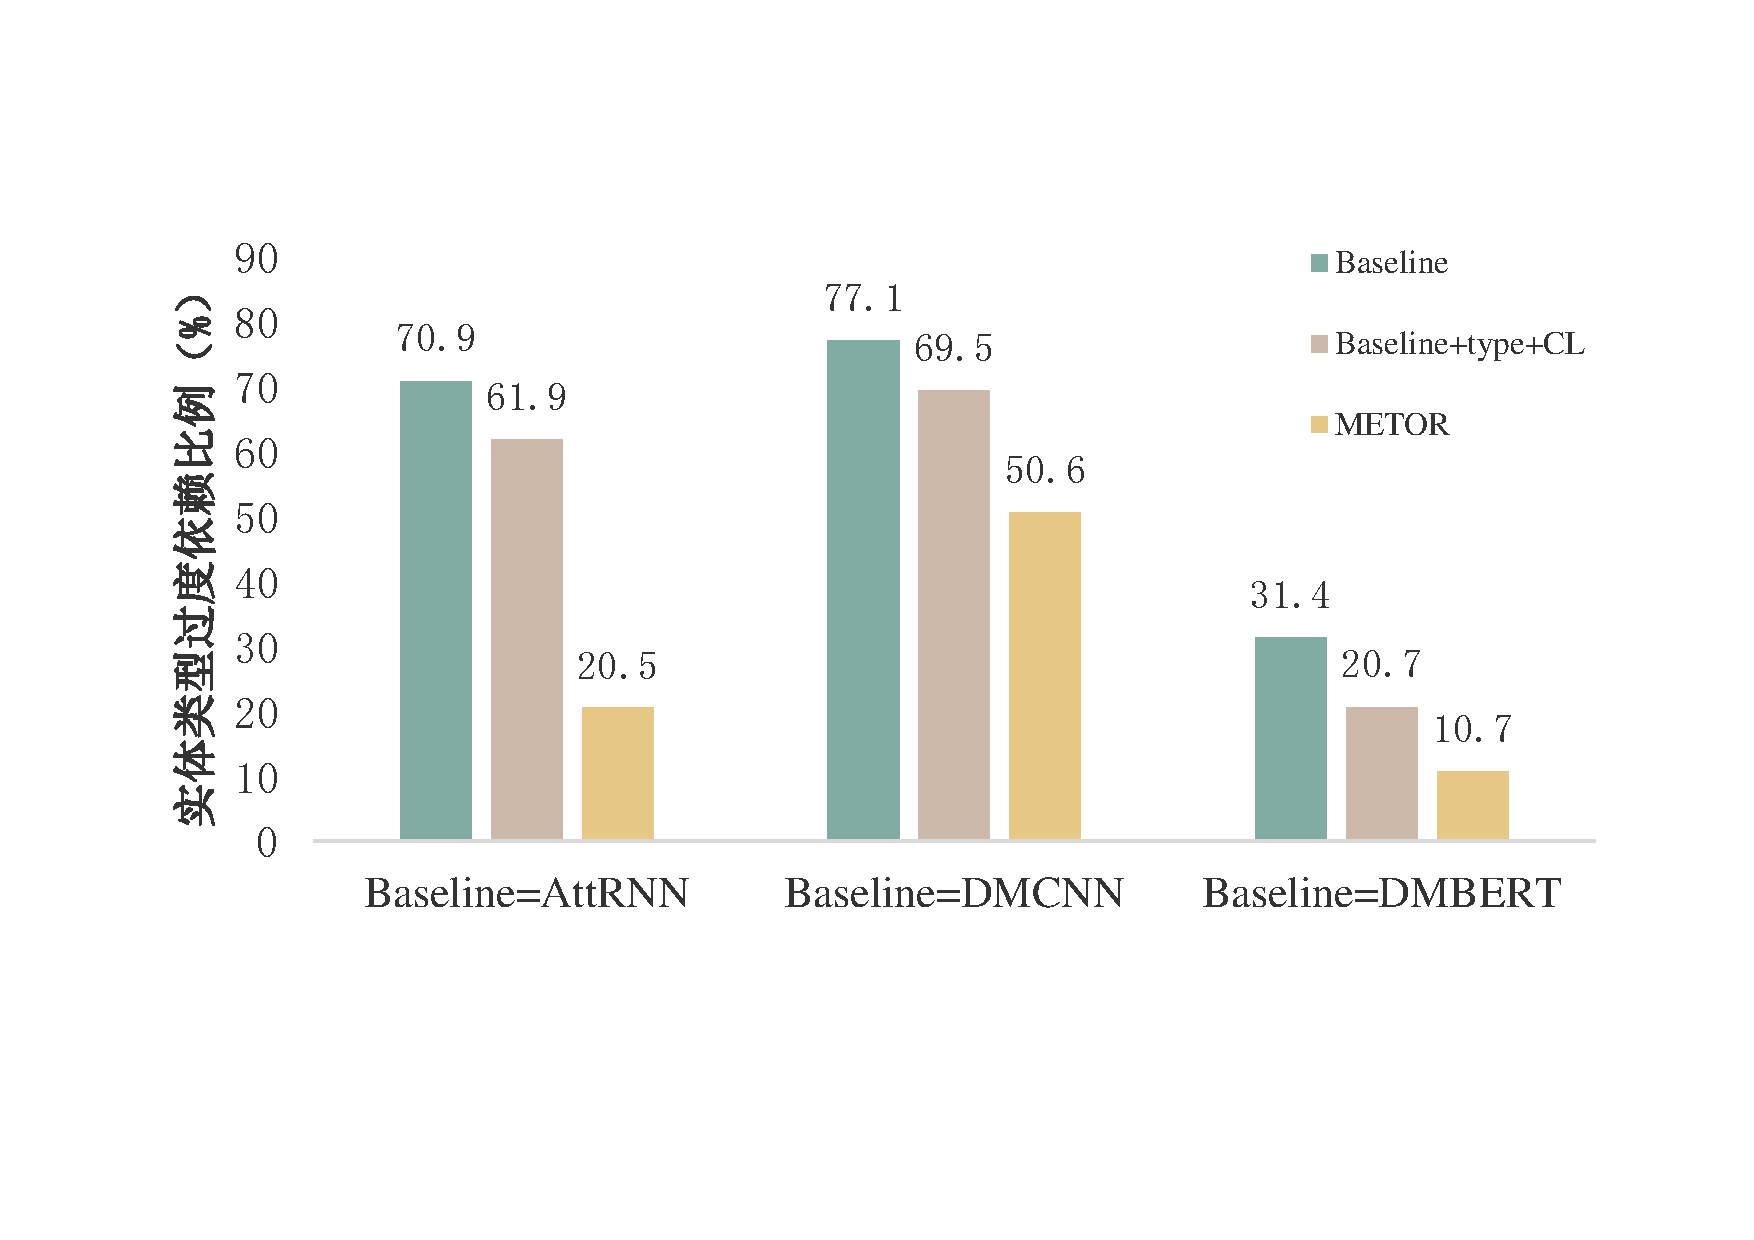
\includegraphics[width=0.8\linewidth]{figures/chap4/comparison.pdf}
\caption{不同模型的实体类型过度依赖程度比较}
\label{fig-comparison}
\end{figure}

\subsection{超参数敏感性分析}
本章分析不同超参数对METOR模型性能的影响,包括公式\ref{nt_loss}中的温度参数$\tau$、公式\ref{eq21}中的边际参数$\gamma$和公式\ref{eq24}中的循环训练频率$f$。

如图\ref{temperature}所示,METOR模型在温度参数$\tau$为0.1时性能最佳。当其在0.02到0.5的范围内变化时,METOR模型的F1性能变化幅度不超过1.1\%,这证明了METOR模型在不同$\tau$的设置下的鲁棒性。

从图\ref{margin}中可以观察到,当边际参数$\gamma$设置为0.1时,METOR模型的F1指标性能达到最佳。当边际参数$\gamma$设置为0.05时,从负样本角度消解实体类型过度依赖问题的程度存在不足,METOR模型的F1的性能略有下降。而当边际参数 $\gamma$大于0.1时,其性能也会下降。这是由于给定实例和伪正样本集合中的负样本之间的特征表示过度相似,导致正样本处理模块和负样本处理模块间的训练目标差距较大。然而,由于METOR模型中的循环训练策略能够极大缓解由较大边际参数$\gamma$引起的训练目标不一致性问题,其性能的下降较为有限。

从图\ref{frequency}中可以观察到,当循环训练频率$f$设置为3时,METOR模型实现了最佳性能。当循环频率$f$设置为2时,循环训练策略中主任务和辅助任务的训练频率没有差异,导致METOR模型在两个不一致的训练目标间频繁切换,从而性能出现下降。此外,当循环频率$f$大于3时,导致循环训练策略中负样本处理模块的训练频率较低,其将接近于退化为不包含负样本处理模块的METOR模型。

\begin{figure*}[t]
\centering
\subfigure[]{
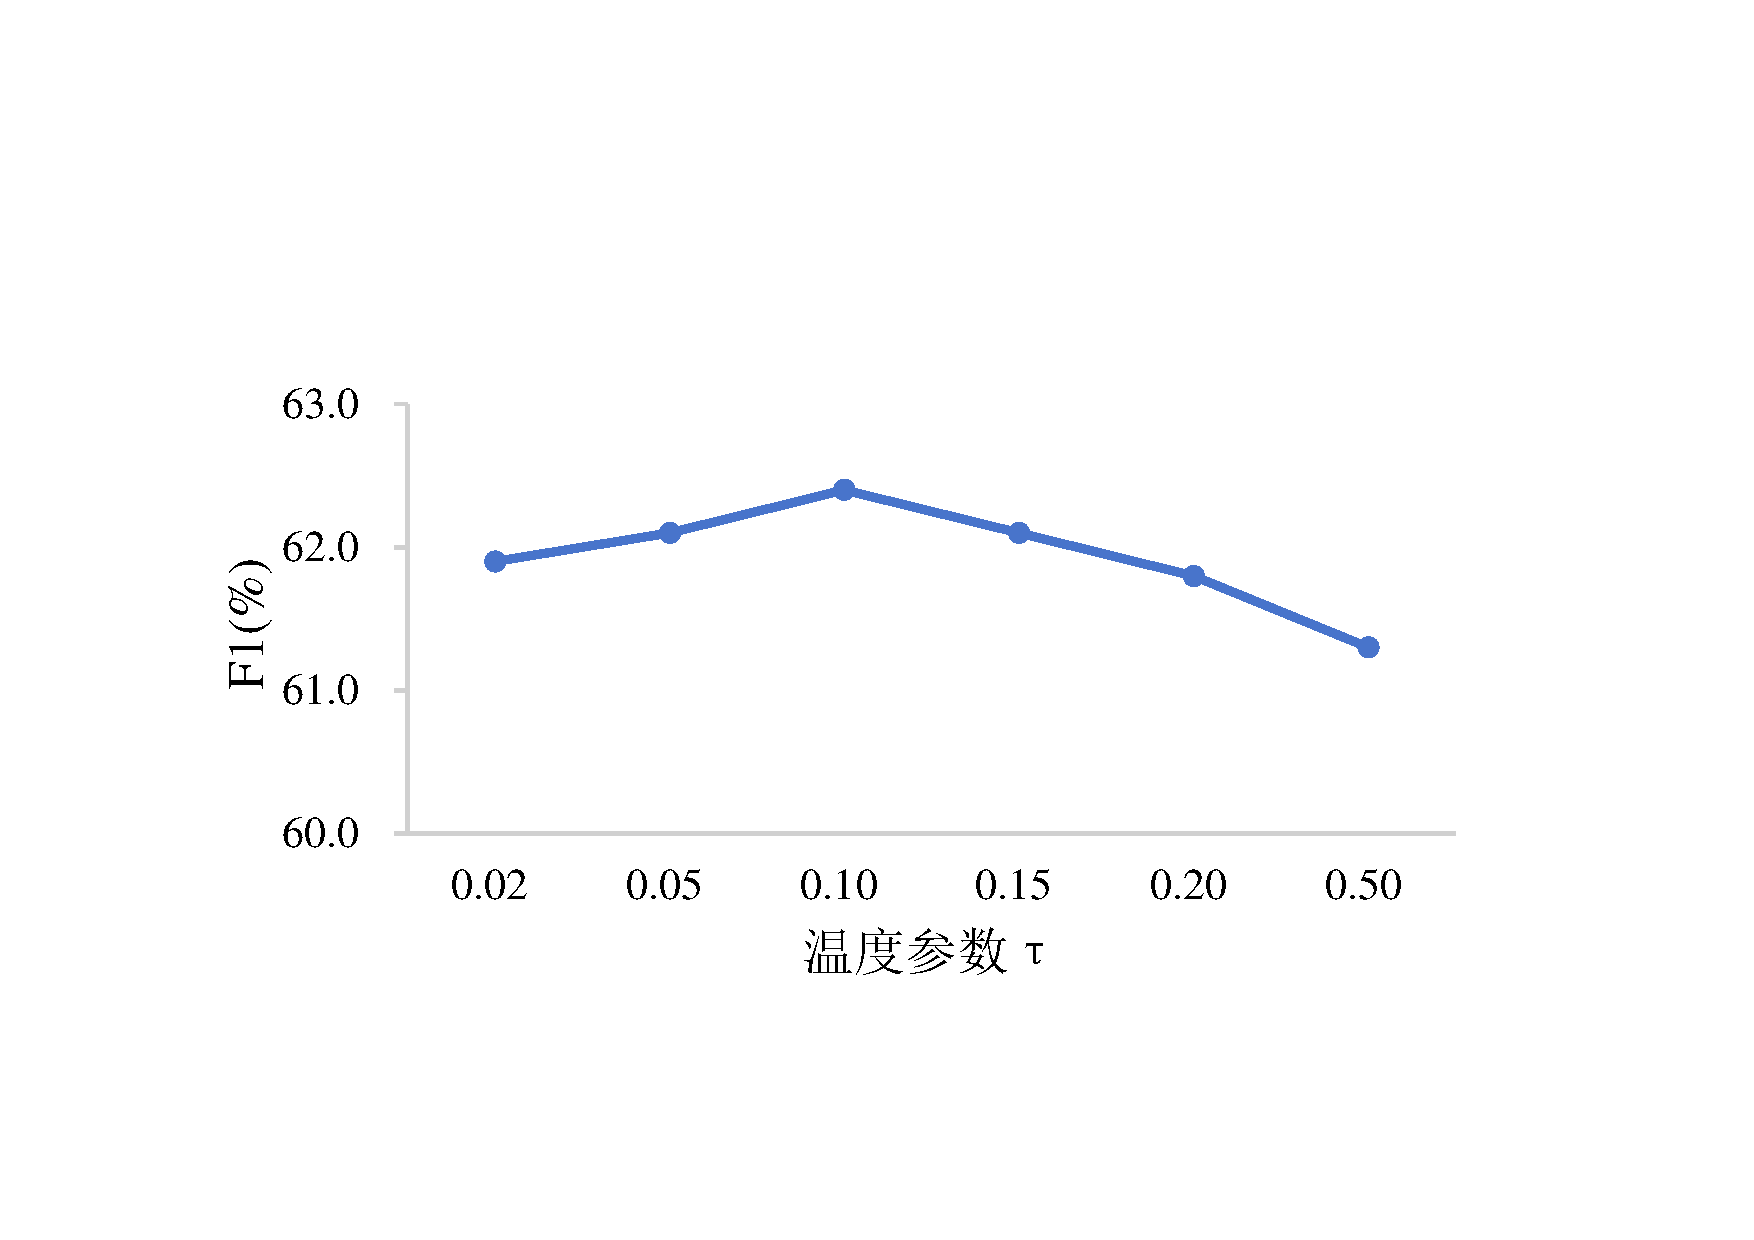
\includegraphics[width=0.6\linewidth]{figures/chap4/temperature.pdf}
\label{temperature}
%\caption{fig1}
}
\quad
\subfigure[]{
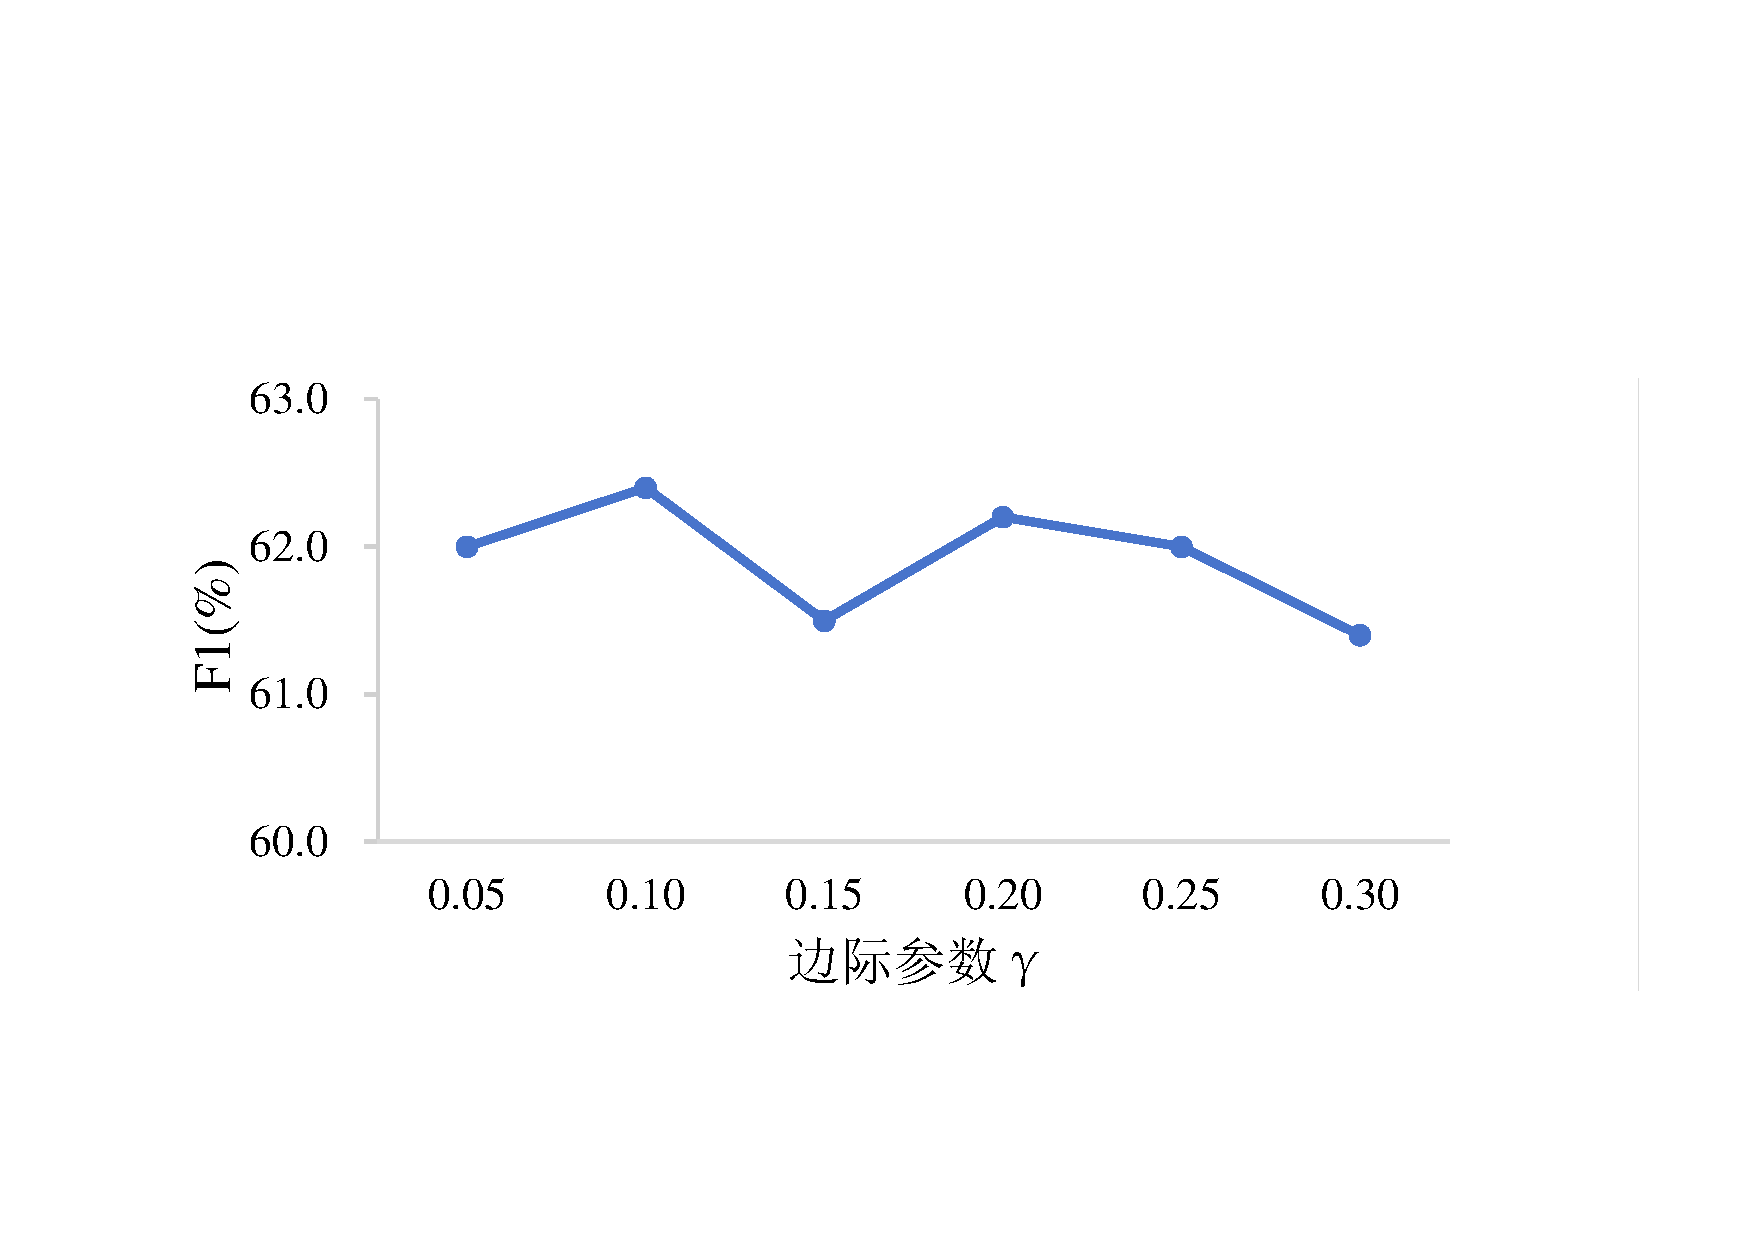
\includegraphics[width=0.6\linewidth]{figures/chap4/margin.pdf}
\label{margin}
}
\quad
\subfigure[]{
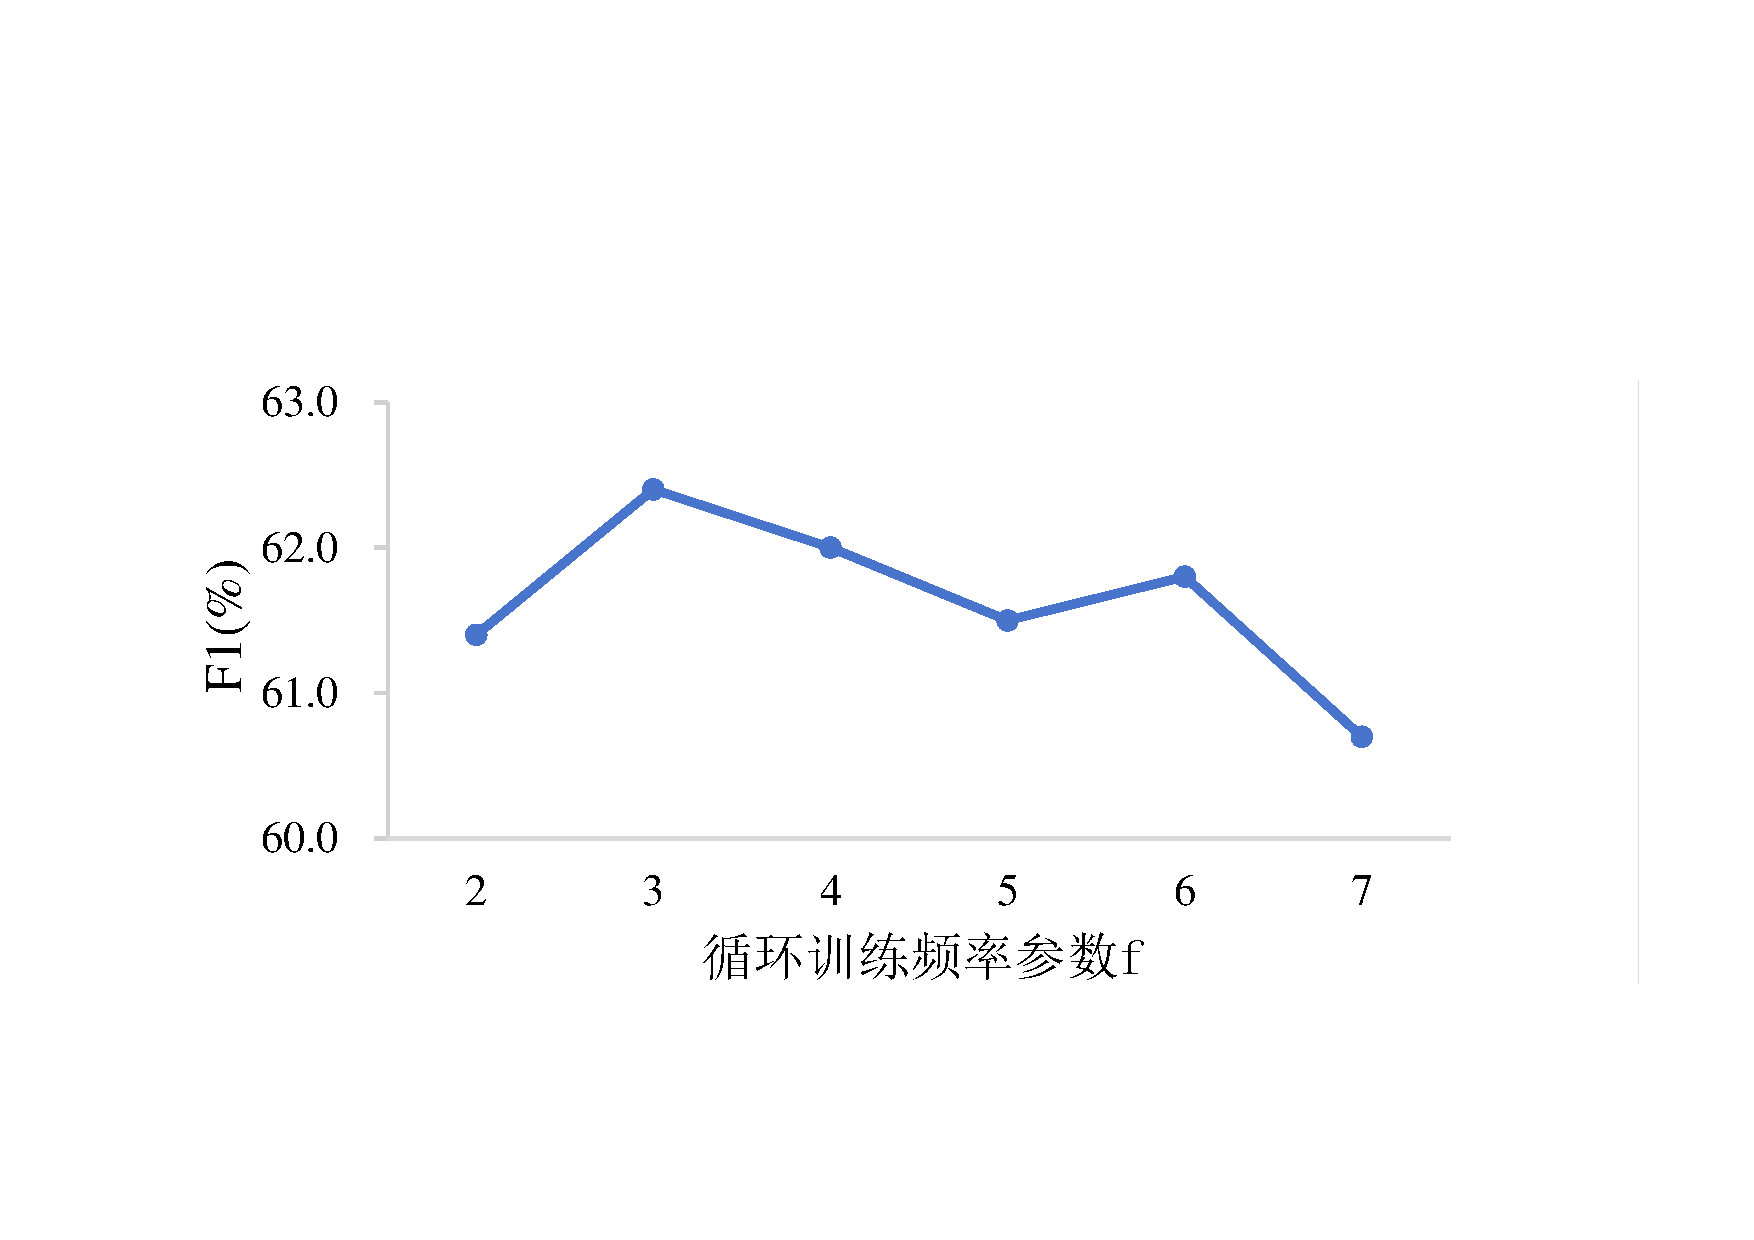
\includegraphics[width=0.6\linewidth]{figures/chap4/frequency.pdf}
\label{frequency}
}
\caption{METOR模型参数敏感性分析}
\label{sensitivity}
\end{figure*}

\subsection{计算复杂度分析}
虽然本章所提方法在实验中应用到了不同的事件要素抽取模型,但计算复杂度的分析是相似的。因此,本节着重讨论基于DMBERT的METOR模型的情况,具体计算如下:在编码器模块中,BERT的计算复杂度主要来源于多头注意力~\cite{vaswani2017attention},为$O~(N^2 d+Nd^2)$,其中$N$是输入序列的最大长度,$d$是BERT隐藏层输出向量的维度。在正样本处理模块中,语义相关性信息的计算复杂度为$O~((d_{s}^2 +d_{s})n_{e})$,其中$d_{s}$是事件类型/实体类型/要素类型向量的维度,$n_{e}$是给定事件要素抽取数据集中预定义实体类型的数目。对于基于NT-Xent的对比学习来说,其计算复杂度为$O~((d+d_{s}+d_{2})d_{1}+K d_{2}+K^{2})$,其中$d_{1}$和$d_{2}$是维度参数,$K$是批数据大小。在负样本处理模块中,计算复杂度为$O~(d_{2})$。在循环训练策略模块中,多类分类器的计算复杂度为$O~(n_{r}(d+d_{s}))$,其中$n_{r}$是给定事件要素抽取数据集中预定义要素类型的数目。

因此,METOR模型的总计算复杂度为$O~(N d^{2}+(N^{2}+d_{1}+n_{r})d+(d_{1}+K)d_{2}+n_{e}d_{s}^2+(d_{1}+n_{r}+n_{e})d_{s}+K^2)$。如果忽略较小的参数$n_{e}$, $n_{r}$和$d_{s}$,则其计算复杂度可以简化为$O~(N d^{2}+(N^{2}+d_{1})d+(d_{1}+K)d_{2}+K^2)$。进一步,与计算复杂度为$O~(N d^{2}+N^{2}d)$的基线模型DMBERT相比,所提模型的计算复杂度增长了$O~(d_{1} d+(d_{1}+K) d_{2}+K^2)$。由于在本章的超参数设置中,存在$d_{1}+K<d$,$d_{2}<d$和$K < N$,使得增长的计算复杂度$O~(d_{1} d+(d_{1}+K) d_{2}+K^2)$约等于$O~(d^{2}+N^{2})$。因此,可以得知METOR模型的计算复杂度略高于DMBERT,但其F1性能显著提高了5.2\%。

\subsection{案例研究}
本章节选取ACE2005数据集测试集中的六个实例进行案例研究。表\ref{case}展示了使用DMBERT、DMBERT(CL)和本章所提的METOR模型对这些实例的预测结果,其中DMBERT(CL)为表\ref{analysis}中的变体模型DMBERT+type+CL。

\begin{table*}[htp]
\footnotesize
\centering
% \setlength{\abovecaptionskip}{0pt}
% \setlength{\belowcaptionskip}{10pt}
\caption{ACE2005数据集上的案例分析}
% The trigger words and event argument candidates are in red and blue, respectively.}
\begin{tabular}{lcccc}
\toprule
\multicolumn{1}{c}{实例}    & 实体类型  & DMBERT & DMBERT (CL)  & METOR \\ \midrule
\begin{tabular}[c]{@{}l@{}}(1) Liana Owen drove 10 hours from \\ Pennsylvania to attend the \textcolor{red}{rally} in \\ \textcolor{blue}{Manhattan} with her parents.\end{tabular}              & County-or-District & Place $\checkmark$     &  Place $\checkmark$   & Place $\checkmark$     \\ \midrule
\begin{tabular}[c]{@{}l@{}}(2) He asked \textcolor{blue}{the court} to invalidate \\ the \textcolor{red}{verdict} and throw out the criminal \\ case against Pasko.\end{tabular} & Government & Adjudicator $\checkmark$ & Adjudicator $\checkmark$ & Adjudicator $\checkmark$ \\ \midrule
\begin{tabular}[c]{@{}l@{}}(3) Separately, \textcolor{blue}{former WorldCom} \\ \textcolor{blue}{CEO Bernard Ebbers} failed on April \\ 29 to make a first repayment of 25 \\ million dollars on a 400-million-dollar \\ \textcolor{red}{loan} from MCI, the Journal said, citing\\ SEC documents.\end{tabular}    & Individual  & Giver $\times$      & Recipient $\checkmark$ & Recipient $\checkmark$      \\ \midrule
\begin{tabular}[c]{@{}l@{}}(4) U.S. Defense Secretary Donald H. \\ Rumsfeld discussed the resolution with \\ Prime Minister Tony Blair and Defense \\ Secretary Geoff Hoon on Friday as \\ Rumsfeld \textcolor{red}{returned} from a tour of Iraq, \\ \textcolor{blue}{Afghanistan} and the Persian Gulf region.\end{tabular}                                    & Nation & Destination $\times$    &  Origin $\checkmark$   & Origin $\checkmark$    \\ \midrule
\begin{tabular}[c]{@{}l@{}}(5) It was not clear \textcolor{blue}{how many people} \\ were in the cafe at the time of the \textcolor{red}{blast}.\end{tabular}                                    & Indeterminate      & None $\times$    &  None $\times$   & Target $\checkmark$    \\ \midrule
\begin{tabular}[c]{@{}l@{}}(6) The space agency has been under \\ intense scrutiny since February when \\  \textcolor{blue}{the space shuttle Columbia} disintegrated \\ over Texas,  \textcolor{red}{killing} all seven crew \\ members.\end{tabular}  & Air     &  Instrument $\times$    &  Instrument $\times$   & None $\checkmark$    \\ \bottomrule
\end{tabular}
\label{case}
\end{table*}

在实例(1)中,“rally”触发了$Demonstrate$事件,且事件候选要素为“Manhattan”,其实体类型和要素类型分别为$County-or-District$和$Place$。由于实体类型$County-or-District$通常以要素类型$Place$参与到事件中,为该要素类型预测提供了重要信息。因此,DMBERT、DMBERT(CL)和本章所提的METOR模型通过实体类型$County-or-District$提供的语义信息给出了正确的要素类型预测。

在实例(2)中,候选事件要素“the court”的实体类型和要素类型分别为$Government$和$Adjudicator$。虽然实体类型$Government$无法提供明显的语义信息来预测要素类型,但当“verdict”触发的$Convict$事件给出时,其可以为预测提供信息提示。换而言之,$Government$实体经常在$Convict$事件中以要素类型$Adjudicator$出现,所以三个模型均能正确预测要素类型。因此,前两个实例证明了实体类型可以为预测其频繁参与的要素类型提供有用的预测线索。

在实例(3)中,在由“loan”触发的$Transfer-Money$事件中,候选事件要素“former WorldCom CEO Bernard Ebbers”的实体类型和要素类型分别为$Individual$和$Recipient$。由于要素类型$Giver$和$Recipient$均与实体类型$Individual$在$Transfer-Money$事件中频繁关联,DMBERT无法在该实例中正确区分$Giver$和$Recipient$。然而,DMBERT(CL)和本章所提的METOR模型均受益于对比学习,避免被同一事件中具有相同实体类型的要素类型所混淆,给出了正确的识别结果。实例(4)展示了另一个类似的实例。

在实例(5)中,候选事件要素“how many people”的实体类型和要素类型分别为$Indeterminate$和$Target$。从语义上来看,如果候选要素为一个$Indeterminate$实体,则该实体很有可能在事件中不作为要素出现。这种强语义关联导致了DMBERT对要素类型的预测错误。进一步,由于多数实体类型为$Indeterminate$的候选要素在训练集中不为
事件要素出现,DMBERT(CL)使用传统的对比学习来避免对于实体类型$Indeterminate$过度依赖的效果不佳。然而,本章所提的METOR模型消解了这种实体类型过度依赖问题,避免了该错误。

在实例(6)中,在由“killing”触发的$Die$事件中,候选事件要素“the space shuttle Columbia”的实体类型和要素类型分别是$Air$和$None$。和实例(5)相似,如果候选事件要素为一个$Air$实体,则该实体很有可能在事件中以要素类型$Instrument$出现,这阻碍了DMBERT和DMBERT(CL)从文本中理解语义信息,导致它们做出错误的预测。与之相比,METOR模型正确预测了要素类型。因此,METOR可以同时减少假负(false negative)预测(如实例(5)所示)和假正(false positive)预测(如实例(6)所示),从而取得优秀的事件要素抽取性能表现。

\section{本章小结}
本章首先研究了事件要素抽取的实体类型依赖性,并利用预实验评估其对不同事件要素抽取基线模型整体性能的影响。预实验表明了不同基线模型均面临不同程度的实体类型过度依赖问题,从而降低了整体性能。为此,本章提出了基于多角度对比学习的实体类型过度依赖消解方法。该方法分别从正样本和负样本角度消解模型在训练过程中对于实体类型的过度依赖,并设计了一种循环训练策略使这两种对比学习方法能够高效协作。本章基于ACE2005数据集进行了充分的实验,结果表明所提方法能够有效地对不同事件要素抽取基线模型进行实体类型过度依赖问题的消解,且当应用在DMBERT基线时,性能显著优于当前最佳的事件要素抽取模型。
%%==================================================
%% chapter01.tex for BIT Master Thesis
%% modified by yang yating
%% version: 0.1
%% last update: Dec 25th, 2016
%%==================================================
% \chapter{基于分离-融合范式的多词元链接事件要素抽取模型}
\chapter{基于分离-融合范式的跨事件信息构建与利用}
\label{chap:chapter5}

以ACE2005数据集为代表的句子级别数据集被主流的事件抽取研究广泛采用,但随着真实世界文本内容的复杂性不断增加,事件要素信息越来越多地跨越出现在一个文档中的多个句子中。因此,研究同时适用于句子级别和文档级别事件要素抽取的通用模型成为新的研究热点和挑战。与上一章节不同,该研究遵循章节\ref{section2_2}所述的关于事件要素抽取的第二种定义,即不使用实体提及的标注信息,而在预测要素类型的同时识别出其文段范围。

现有通用文本级别事件要素抽取模型存在各自的局限性,而基于多词元链接的建模方法能够有效避免这些模型的内在局限,并展现出良好的性能潜力。因此,本章研究利用多词元链接方法进行通用文本级别的事件要素抽取。然而该方法中的单一事件建模方式缺乏对跨事件依赖关系的利用,多事件建模方式需要更长的要素类型序列编码和额外的链接操作,增加了预测推理的难度。为此,本章提出了一种基于分离-融合范式的跨事件信息构建与利用方法,并相应提出了一种新的多词元链接模型,避免了当前方法的各自局限,且实现了从不同级别文本中高效利用跨事件依赖信息。实验结果证明了本章提出的模型在所有句子级和文档级数据集上都优于目前性能最优的事件要素抽取模型。

\section{引言}
\label{introduction}

最近,基于抽取式~\cite{ma2022prompt, he2023revisiting, nguyen2023contextualized, li2023intra}和生成式~\cite{hsu2022degree,du2022dynamic,zhang2023overlap}的提示学习方法在同时适用于句子级别和文本级别的事件要素抽取任务上取得了显著的性能提升。然而,前者在抽取具有相同要素类型的多个事件要素时,受到提示模版中预先设定的重复要素槽位数量的限制,后者在抽取长距离事件要素的性能表现不佳。此外,这两类方法的性能表现均较为依赖于提示模版的设计质量。

因此,不同于基于提示学习的方法,最近的一些研究~\cite{wang2022query,lou2023universal,liu2023rexuie}将输入文本和所有涉及的要素类型串接成自然语言序列,然后联合编码,并进一步实施多词元\footnote{“词元”对应于英文表达中的“token”,这里特指经过预训练语言模型分词器分词后得到的语义单元。}链接操作,从而实现事件要素抽取或通用信息抽取的建模。其中,所有事件要素文段和要素类型的并行链接操作能够直接高效地抽取具有相同要素类型的多个事件要素,并提升长文本中分散的事件要素间的交互。此外,该类方法不需要精心设计的提示模版。根据每次同时抽取的事件数量,可以进一步将该类方法划分为两种建模方式:单事件抽取和多事件抽取。

第一种方式的研究~\cite{wang2022query,liu2023rexuie}将待抽取文本和只在目标事件中出现的要素类型串接后作为输入,然后实施两种链接操作去建模目标事件。如图\ref{example}所示,其中被红色标记的为事件触发词,被黄色标记的为事件要素类型,不同颜色的箭头表示不同种类的链接操作,事件要素“James McDade”在$Die$事件和$Attack$事件中扮演了不同的要素类型,其抽取建模过程是分离的。虽然这种单事件抽取的方式便于进行简单的链接预测,但其忽略了建模不同事件间的显著关联依赖~\cite{zeng2022ea2e,he2023revisiting,li2023intra}。

\begin{figure}[htp]
\centering
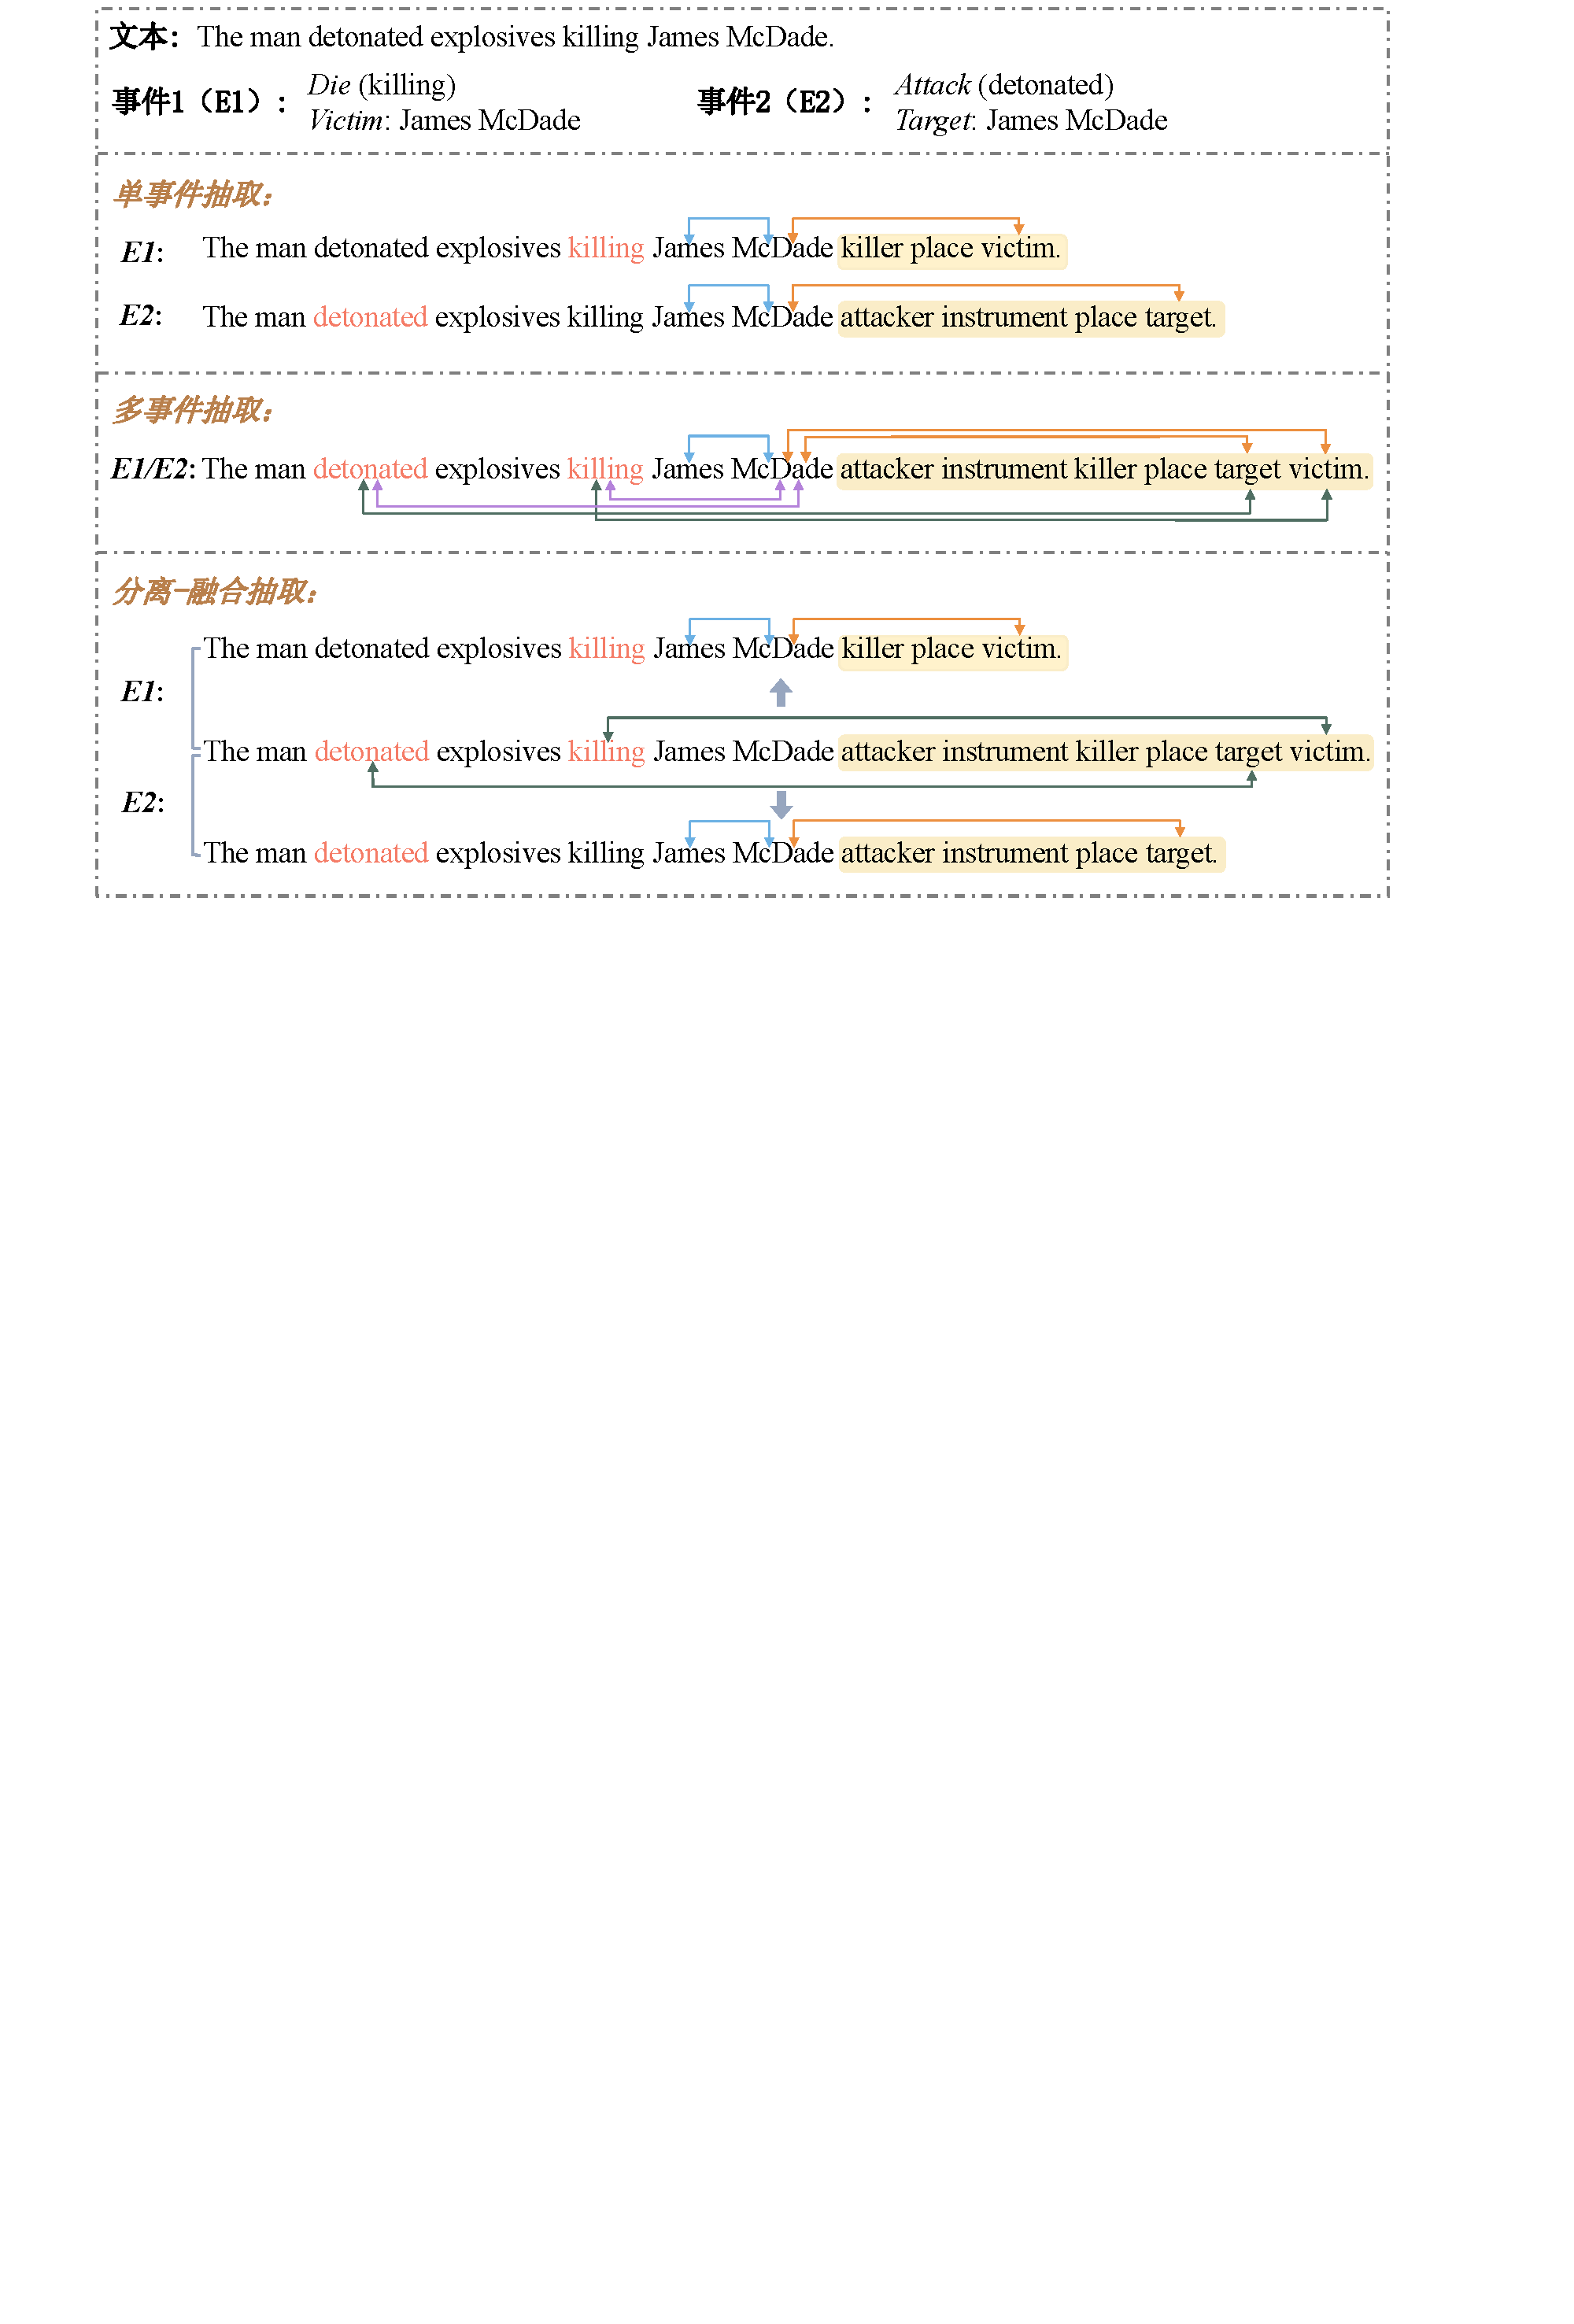
\includegraphics[width=1\columnwidth]{figures/chap5/introduction.pdf} 
\caption{基于不同建模方式的多词元链接事件要素抽取示意图}
% \emph{E1}: \emph{Event 1}. \emph{E2}: \emph{Event 2}. The trigger words are highlighted in red, the concatenated roles are in yellow, and the arrows of different colors represent different linking operations. Note that we only exhibit one argument of each event for simplification.}
\label{example}
\end{figure}

因此,第二种方式的研究~\cite{lou2023universal}一次性抽取多个事件的事件要素。然而,两个新的问题随之而来。首先,与输入文本串接的不再是只在单个事件中出现的要素类型,而是在所有事件中出现的要素类型,这使得通过链接预测选择出正确的要素类型变得更加困难。其次,与单事件抽取方式相比,其需要两种额外的链接操作来确定抽取的事件要素文段和对应的要素类型归属的事件触发词,导致预测阶段积累更多的错误。图\ref{example}展示了同时从$Die$事件和$Attack$事件中抽取事件要素“James McDade”时,其额外增加的触发词-要素文段和触发词-要素类型链接操作。

为了利用上述两种抽取方式的优点,本章设计了一种基于分离-融合范式的跨事件信息构建与利用方法,其先分离跨事件信息获取和事件要素抽取的过程,然后将获取的跨事件信息融合到最终的事件要素抽取中。通过这种分离-融合范式,最终的事件要素抽取可以同时保留单事件抽取方式的简单链接预测和多事件抽取方式的跨事件依赖关系建模能力。图\ref{example}说明了这一范式,其中中间部分从事件要素抽取过程中分离出来,通过触发词-要素类型链接获取跨事件信息,向上和向下的箭头表示跨事件信息的融合。

遵循设计的范式,本章提出了一种新颖的多词元链接事件要素抽取模型去获取分离的跨事件信息并进一步两阶段地融合到最终的事件要素预测(\textbf{Sep}arate acquisition of cross-event information and \textbf{Two}-fold \textbf{F}usion,Sep2F)。为了分离跨事件信息获取和事件要素抽取过程,本章设计了两个多词元链接模块。具体来说,针对多事件中的每个事件,引入一个链接模块来连接事件触发词和其中出现的要素类型。因此,不同事件触发词的特征表示并行聚合了在各自事件中出现的所有要素类型,提供了关键的跨事件信息。同时,引入另一个链接模块抽取目标事件的事件要素。其利用两种链接操作获取事件要素的文段范围和对应的要素类型。在此基础上,本章提出了一个两阶段融合模块将获取的跨事件信息融合到目标事件的要素抽取中。具体地,其首先动态融合来自上述两个链接模块的文本特征表示。然后,利用融合的文本特征表示获取跨模块词元链接分数。该链接分数被进一步融合到最终的预测中。这两阶段的融合过程相互影响,提供了显著的性能贡献。本章的主要贡献可以概括如下:

\begin{itemize}
\item 提出了一种新的基于分离-融合范式的跨事件信息构建与利用方法,其能够同时建模跨事件依赖信息和保留单事件抽取方式的优点。
\item 基于分离-融合范式,提出了一种新的多词元链接事件要素抽取模型,其避免了当前通用事件要素抽取方法的各自局限,且实现了从不同级别文本中通用高效地利用跨事件信息。具体地,设计了两个链接模块,以分别获取跨事件信息和抽取目标事件的事件要素。此外,引入了一个两阶段融合模块,以确保在要素抽取过程中充分利用到获取的跨事件信息。
\item 在四个不同文本级别的数据集上进行了充分的实验,实验结果表明本章所提的模型均显著超越目前性能最优的事件要素抽取基线方法。
\end{itemize}

\section{方法设计}

本章使用$(X,T,C)$表示每个数据实例,其中$X$是输入文本,$T$是目标事件,$C$表示在文本$X$中除目标事件$T$以外的其他事件。具体地,$T$进一步表示为 $\left(e,t,\mathcal{R}^{e}\right)$,其中$e$是事件类型,$t$是事件触发词,$\mathcal{R}^{e}$为只在事件$e$中出现的要素类型集合。类似地,$C$可表示为
$\{(\tilde{e}_i,\tilde{t}_i,\mathcal{R}^{\tilde{e}_i})|~i \leq |C|\}$,其为目标事件$T$提供了跨事件信息。基于此,本章所提模型旨在抽取目标事件$T$的要素集合$\mathcal{A}$,其集合$\mathcal{A}$中的每个事件要素$a^{(r)}$表示要素类型为$r \in \mathcal{R}^{e}$的$X$中文本片段。

如图\ref{framework-sep2f}所示,本章提出的模型由三个模块组成:多事件链接构造、目标事件链接构造和两阶段融合,其遵循了本章设计的分离-融合范式。具体地,前两个模块将跨事件信息的获取和目标事件的要素抽取过程分离,最后一个模块实现了获取的跨事件信息的融合。接下来,本章将具体介绍各个模块。

\begin{figure*}[htp]
\centering
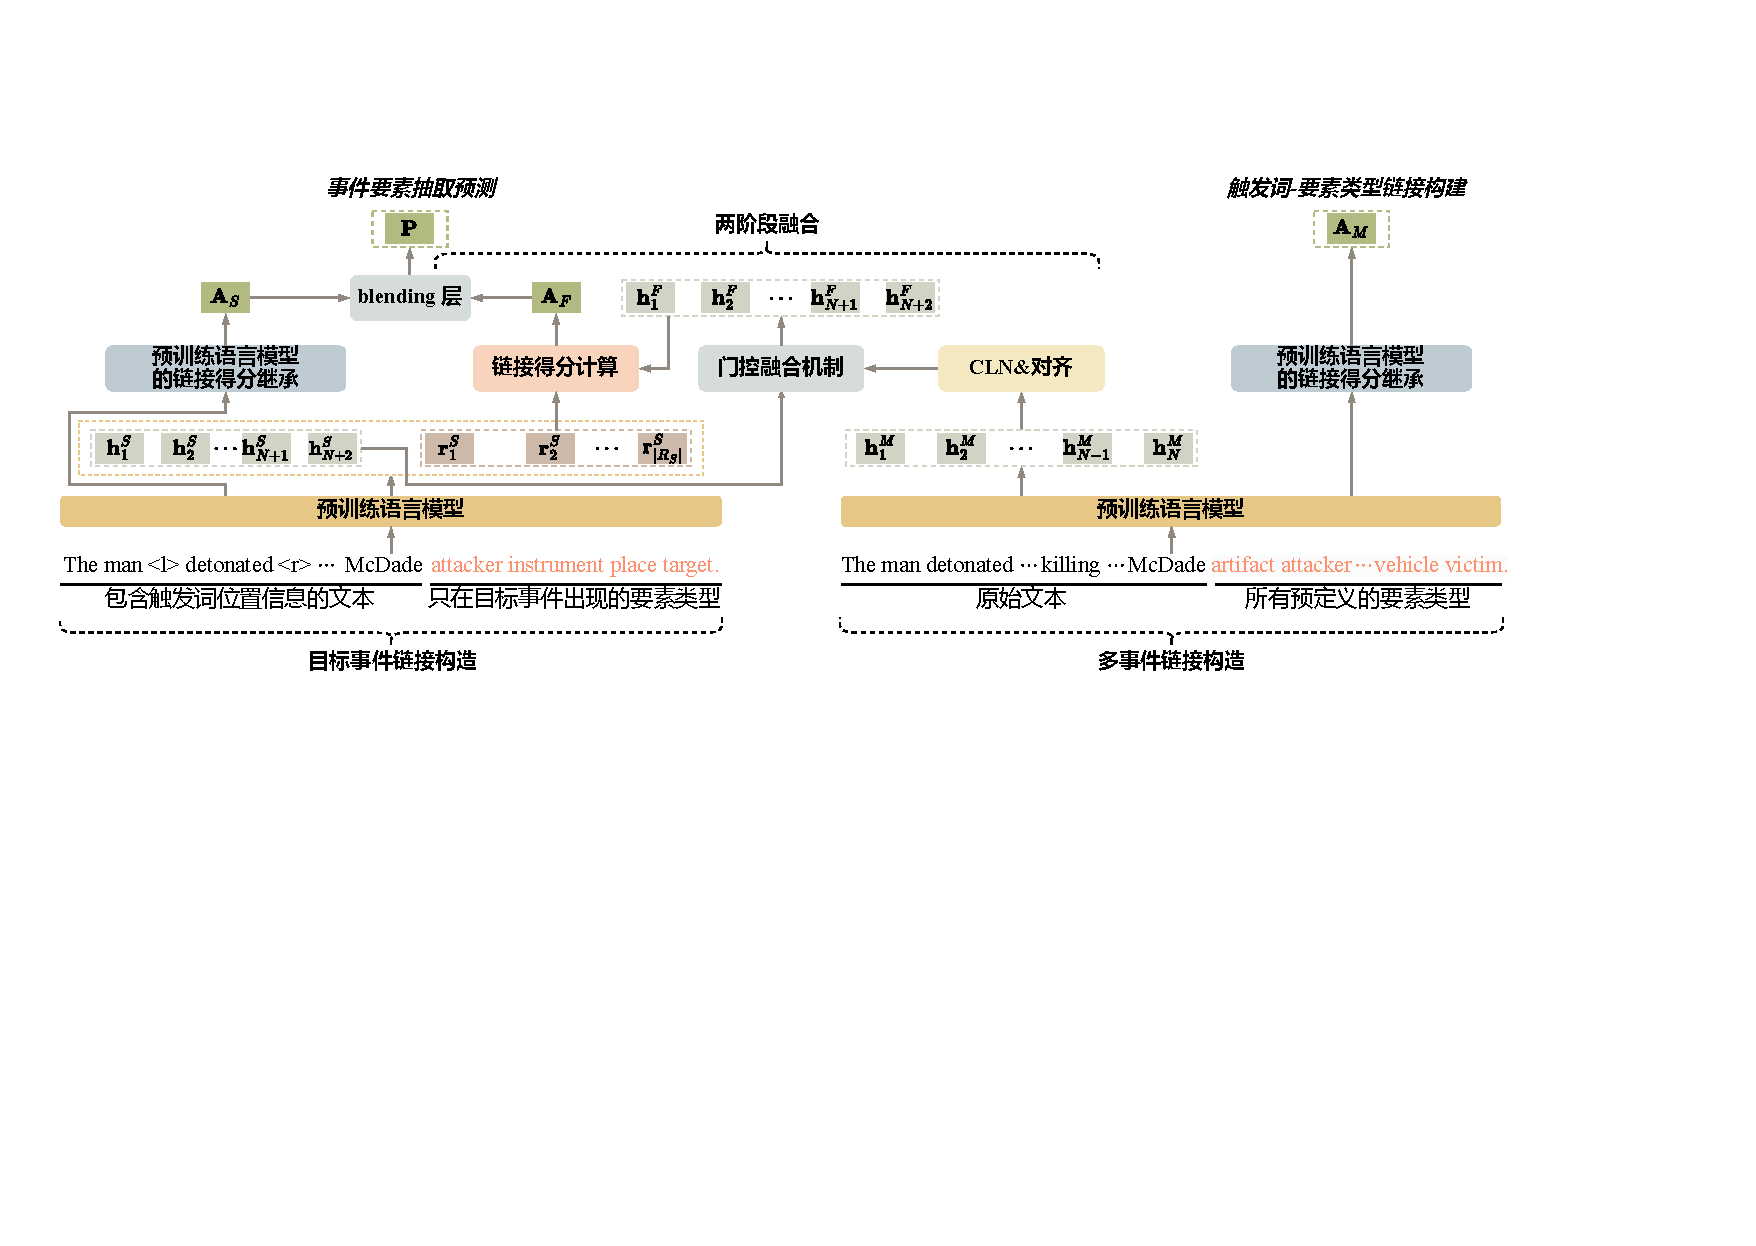
\includegraphics[width=1\linewidth]{figures/chap5/framework.pdf}
\caption{Sep2F模型架构图}
\label{framework-sep2f}
\end{figure*}

\subsection{多事件链接构造}
本模块通过聚合多事件的要素类型信息来获取跨事件信息,其中多事件包含目标事件$T$和所有其他事件$C$。为了实现这种信息聚合,本模块并行地建立不同的事件触发词和它们对应的事件要素类型之间的链接。首先,联合编码待抽取文本和给定数据集中预定义的所有要素类型。然后,根据事件中的触发词-要素类型链接引入标签矩阵和得分矩阵。最后,给出相应的训练损失。

\textbf{编码}~首先,本章利用对应的事件要素名称描述每个事件要素类型,即单个自然语言描述的词。对于名称中包含多个词的少数要素类型,本模型在训练过程中学习额外的特殊词元进行表示。然后,拼接给定数据集中预定义的所有要素类型的名称描述,记作$R_{M}$。在此之后,使用预训练语言模型(PLM)对序列$R_{M}$和输入文本$X$进行联合编码如下:
\begin{equation}
\boldsymbol{E}^{M} = (\boldsymbol{h}_{1}^{M}, \cdots, \boldsymbol{h}_{N}^{M}, \boldsymbol{r}_{1}^{M}, \cdots, \boldsymbol{r}_{|R_{M}|}^{M}) =\textrm{PLM}(X \oplus R_{M})
\end{equation}
其中$\boldsymbol{h}_{n}^{M} \left(1 \leq n \leq N\right)$和 $\boldsymbol{r}_{n}^{M} \left(1 \leq n \leq |R_{M}|\right)$分别为输入文本$X$和事件要素序列$R_{M}$中的词元向量。

\textbf{标签矩阵}~为了学习到多事件各自的要素类型信息,本模块设计了标签矩阵$\boldsymbol{L}_{M} \in {\mathbb{B}}^{(N+|R_{M}|) \times (N+|R_{M}|)}$。对于$T$或$C$中的每个事件,假设其触发词的开始和结束词元向量分别是
$\boldsymbol{h}_{i}^{M}$和$\boldsymbol{h}_{j}^{M}$。进一步,对于该事件中出现的每个要素类型,假设其对应的词元向量是$\boldsymbol{r}_{k}^{M}$。然后,实施链接操作来连接触发词和该要素类型。具体来说,分别构造链接词元对$(i,k+N)$和 $(k+N,j)$,并相应地设置${L}_{M}[i][k+N]$和${L}_{M}[k+N][j]$为“\emph{True}”。对于没有链接的词元对,本模块将$\boldsymbol{L}_{M}$中的相应值标记为“\emph{False}”。图\ref{multi_event_label}展示了$\boldsymbol{L}_{M}$的一个示例,其中被红色标记的为事件触发词词元,被黄色标记的为所有预定义的事件要素类型词元,“\textbf{-}”表示“\emph{False}”。根据图\ref{multi_event_label}可知,“detonated”触发的事件中存在要素类型$Target$,而“killing”触发的事件中存在要素类型$Victim$。

\begin{figure}[htp]
\centering
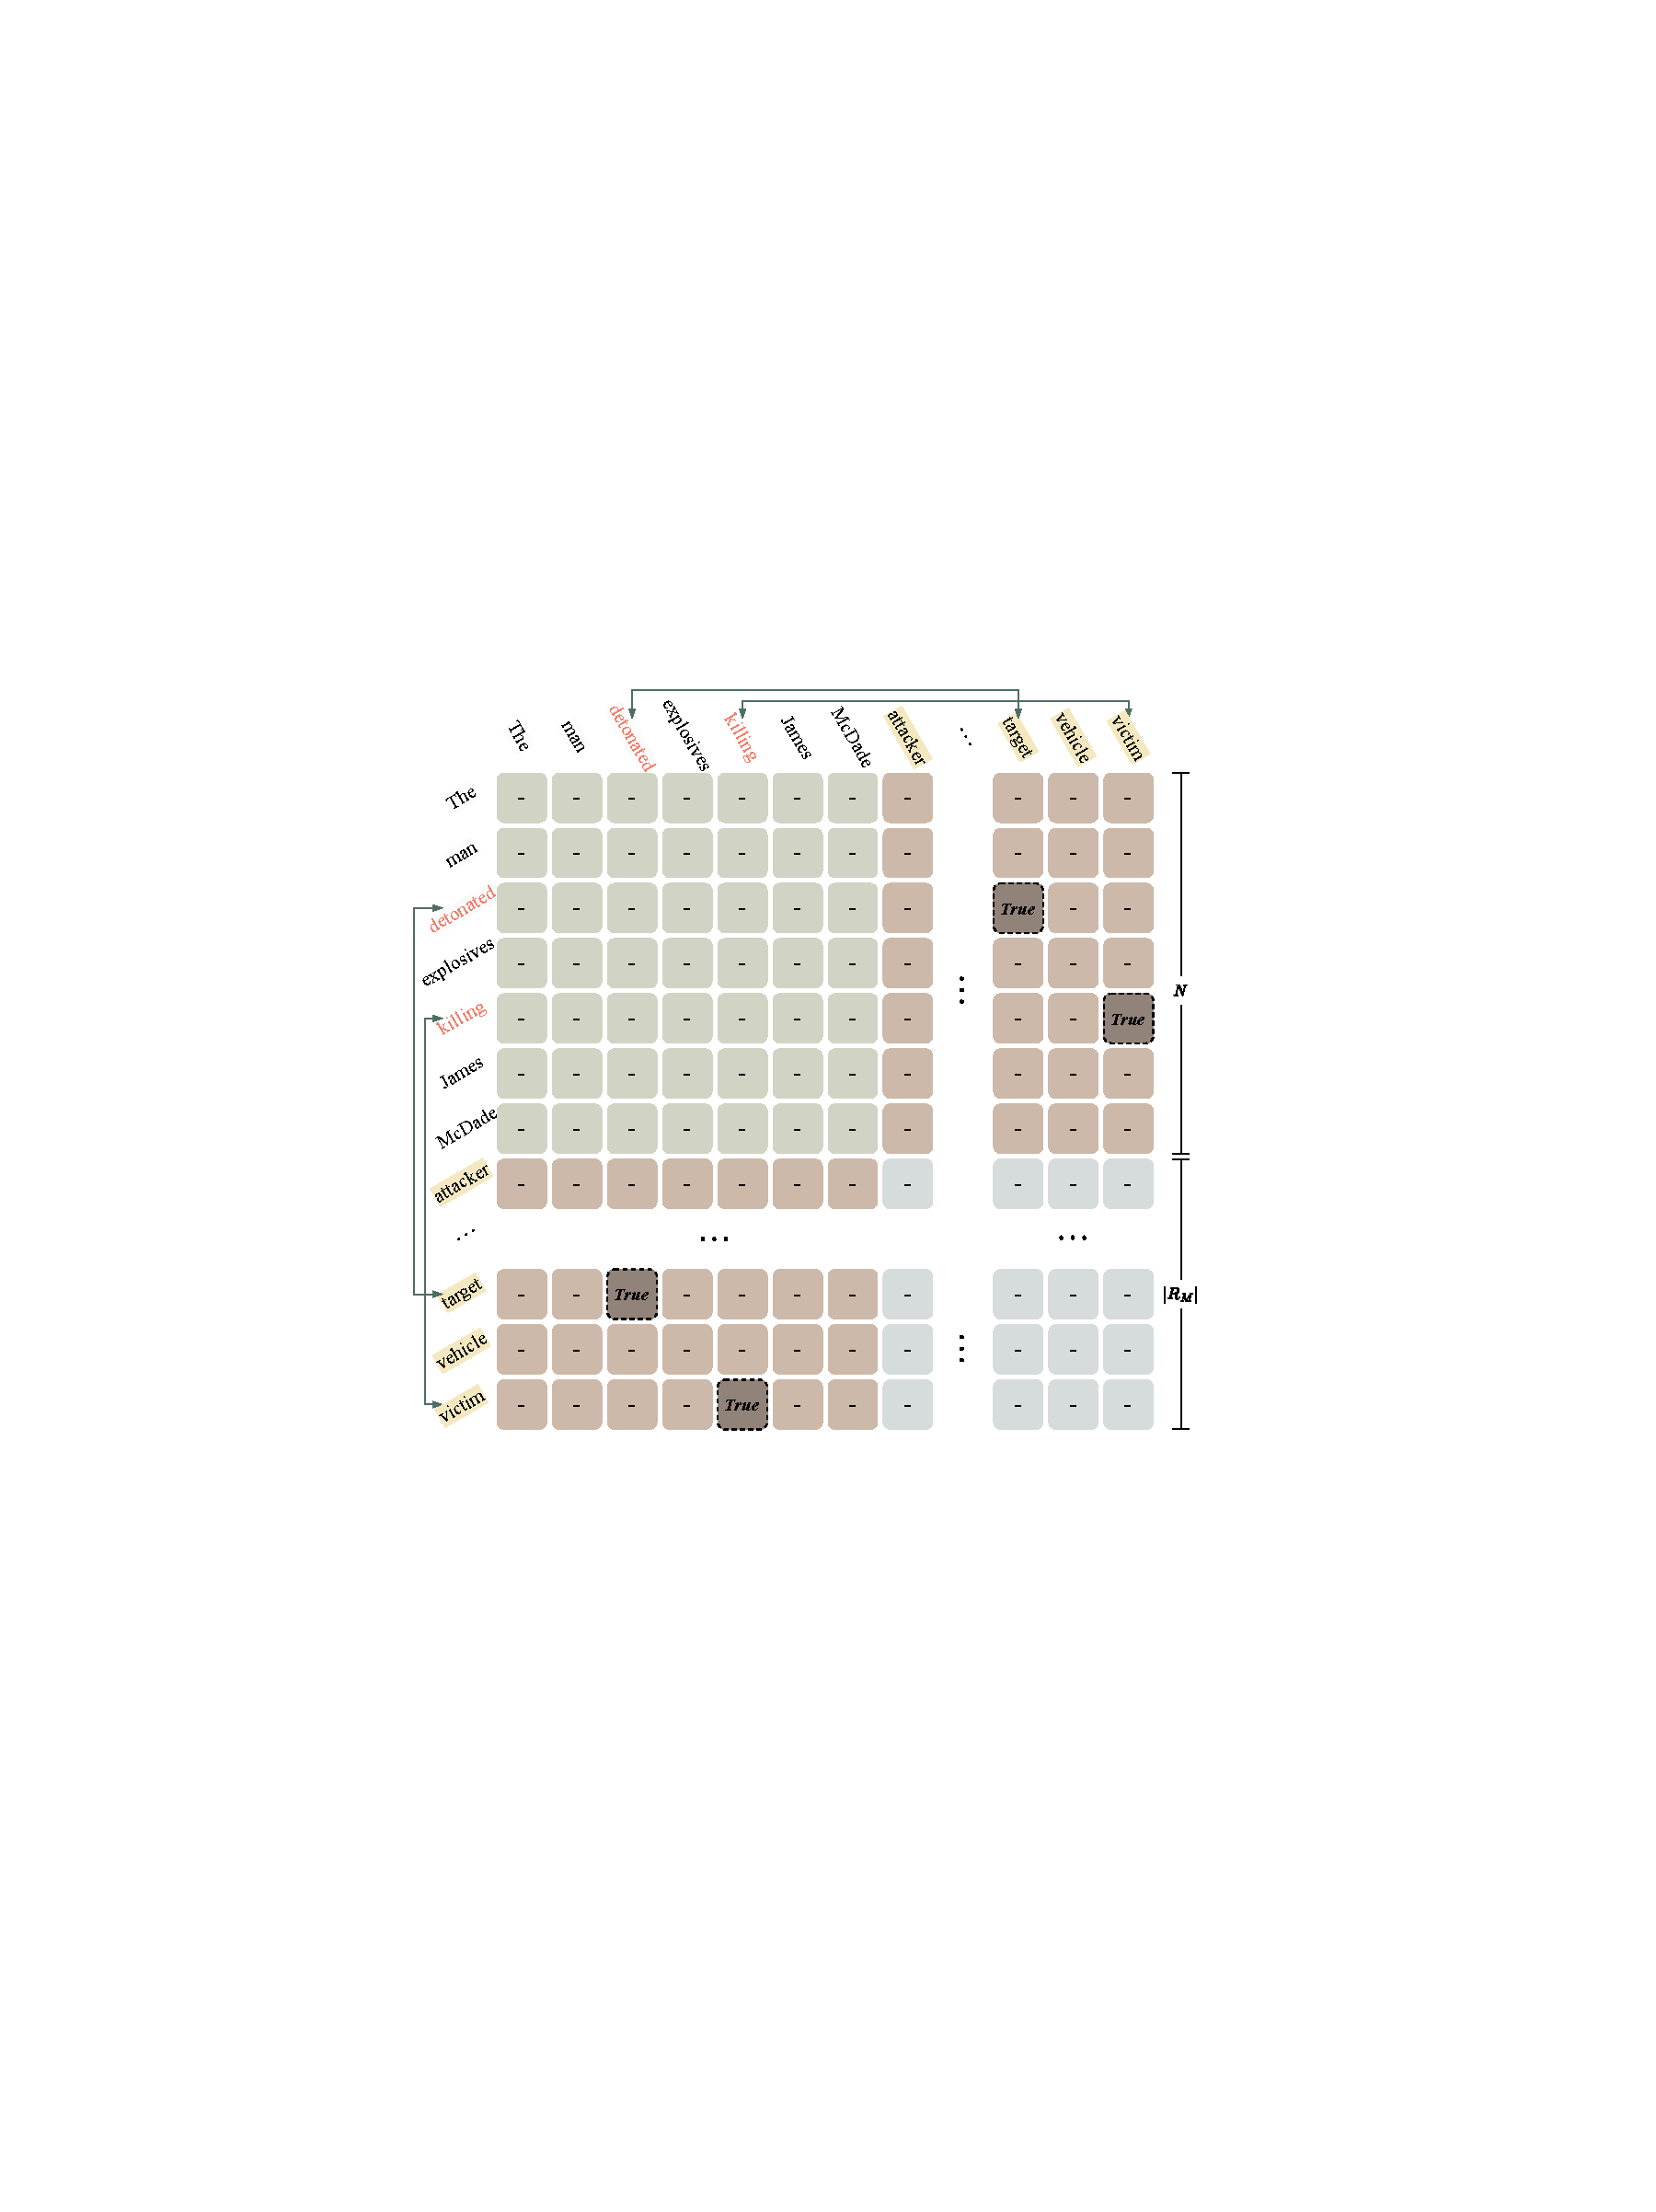
\includegraphics[width=0.6\linewidth]{figures/chap5/label_multi_frame.pdf}
\caption{标签矩阵$\boldsymbol{L}_{M}$示例图}
\label{multi_event_label}
\end{figure}

\textbf{得分矩阵}~受Tang等人~\cite{tang2022unirel}研究工作的启发,本模块继承基于Transformer架构的预训练语言模型的多头自注意力结果作为不同词元对之间的链接分数。具体来说,根据选定的预训练语言模型的最后一层,获取其未经过softmax归一化的多头自注意力权重,并进行均值计算:
\begin{equation}
\boldsymbol{A}_{M}=\frac{1}{P} \sum_p^P \frac{\boldsymbol{Q}_{p} \boldsymbol{K}_{p}^\top}{\sqrt{d_h}}
\label{scores}
\end{equation}
其中$P$为多头的数目,$d_h$为多头自注意机制中查询向量和键向量的维度,$\boldsymbol{Q}_{p}$和$\boldsymbol{K}_{p}$分别为查询矩阵和键矩阵,$\boldsymbol{A}_{M} \in {\mathbb{R}}^{(N+|R_{M}|) \times (N+|R_{M}|)}$表示多事件的触发词-要素类型链接得分。

\textbf{训练损失}~本模块使用训练损失$\mathcal{L_\textrm{TR}}$去指导模型学习不同事件触发词及其相应出现的要素类型之间的链接,如下所示:

\begin{equation}
\begin{split}
    \mathcal{L_\textrm{TR}} = & -\frac{1}{(N+|R_{M}|)^2} \sum_i \sum_j\left(L^{M}_{i,j} \log \sigma\left({A}_{M}[i][j]\right) + \right. \\
    & \left. (1-L^{M}_{i,j}) \log \left(1-\sigma\left({A}_{M}[i][j]\right)\right) \right)
\end{split}
\end{equation}
其中$\sigma(\cdot)$为sigmoid激活函数。当${L}_{M}[i][j]$为“\emph{True}”时,设置$L^{M}_{i,j}$为1,否则设置$L^{M}_{i,j}$为0。

\subsection{目标事件链接构造}
\label{target_event_module}
为了抽取给定目标事件$\left(e,t,\mathcal{R}^{e}\right)$的事件要素,本模块对输入文本和只在事件$e$中出现的要素类型进行联合编码,然后定义对应的多词元链接标签矩阵和得分矩阵,并给出相应的训练损失计算。

\textbf{编码}~与多事件链接构造模块不同,本模块拼接所有$\mathcal{R}^{e}$集合中的事件要素类型的名称描述,记作$R_{S}$。然后,遵循Ma等人~\cite{ma2022prompt}的研究工作在文本$X$中插入两个特殊词元$\langle \ell \rangle$和 $\langle r \rangle$,以便标记触发词$t$的位置:
\begin{equation}
X_{S}=(x_{1},\cdots,\langle \ell \rangle,t,\langle r \rangle,\cdots, x_{|X|})
\end{equation}
在此之后,将包含触发词位置信息的文本$X_{S}$和要素类型序列$R_{S}$进行串接,并利用另一个预训练语言模型对其进行编码:
\begin{equation}
\boldsymbol{E}^{S} = (\boldsymbol{h}_{1}^{S}, \cdots, \boldsymbol{h}_{N+2}^{S}, \boldsymbol{r}_{1}^{S}, \cdots, \boldsymbol{r}_{|R_{S}|}^{S}) =\textrm{PLM}(X_{S} \oplus R_{S})
\end{equation} 
其中$\boldsymbol{h}_{n}^{S} \left(1 \leq n \leq N+2\right)$和$\boldsymbol{r}_{n}^{S} \left(1 \leq n \leq |R_{S}|\right)$分别为$X_{S}$和$R_{S}$中的词元向量。

\textbf{标签矩阵}~为了标记给定目标事件中的事件要素文段范围和要素类型,本模块定义了标签矩阵$\boldsymbol{L}_{S} \in {\mathbb{B}}^{(N+|R_{S}|+2) \times (N+|R_{S}|+2)}$。对于目标事件中的每个事件要素,假设其文段的开始和结束词元向量分别是$\boldsymbol{h}_{i}^{S}$和 $\boldsymbol{h}_{j}^{S}$,其要素类型对应的词元向量是$\boldsymbol{r}_{k}^{S}$。基于此,首先构造链接词元对$(i,j)$和$(j,i)$并设置${L}_{S}[i][j]$和${L}_{S}[j][i]$为“\emph{True}”,以用来标记事件要素的文段。同时,通过要素文段-要素类型链接操作来标记事件要素对应的要素类型信息。相应地,构造两个链接对$(i,k+N+2)$和$(k+N+2,j)$,并设置${L}_{S}[i][k+N+2]$和${L}_{S}[k+N+2][j]$为“\emph{True}”。对于没有链接的词元对,将$\boldsymbol{L}_{S}$中的相应值设置为“\emph{False}”。图\ref{single_event_label}展示了$\boldsymbol{L}_{S}$的一个示例,其中被红色标记的为事件触发词词元,被黄色标记的为只在该事件触发词对应的事件类型中出现的事件要素类型词元,“\textbf{-}”表示“\emph{False}”。根据图\ref{single_event_label}可知,在“detonated”触发的事件中,存在事件要素“James McDade”,其对应的要素类型为$Target$。

\begin{figure}[htp]
\centering
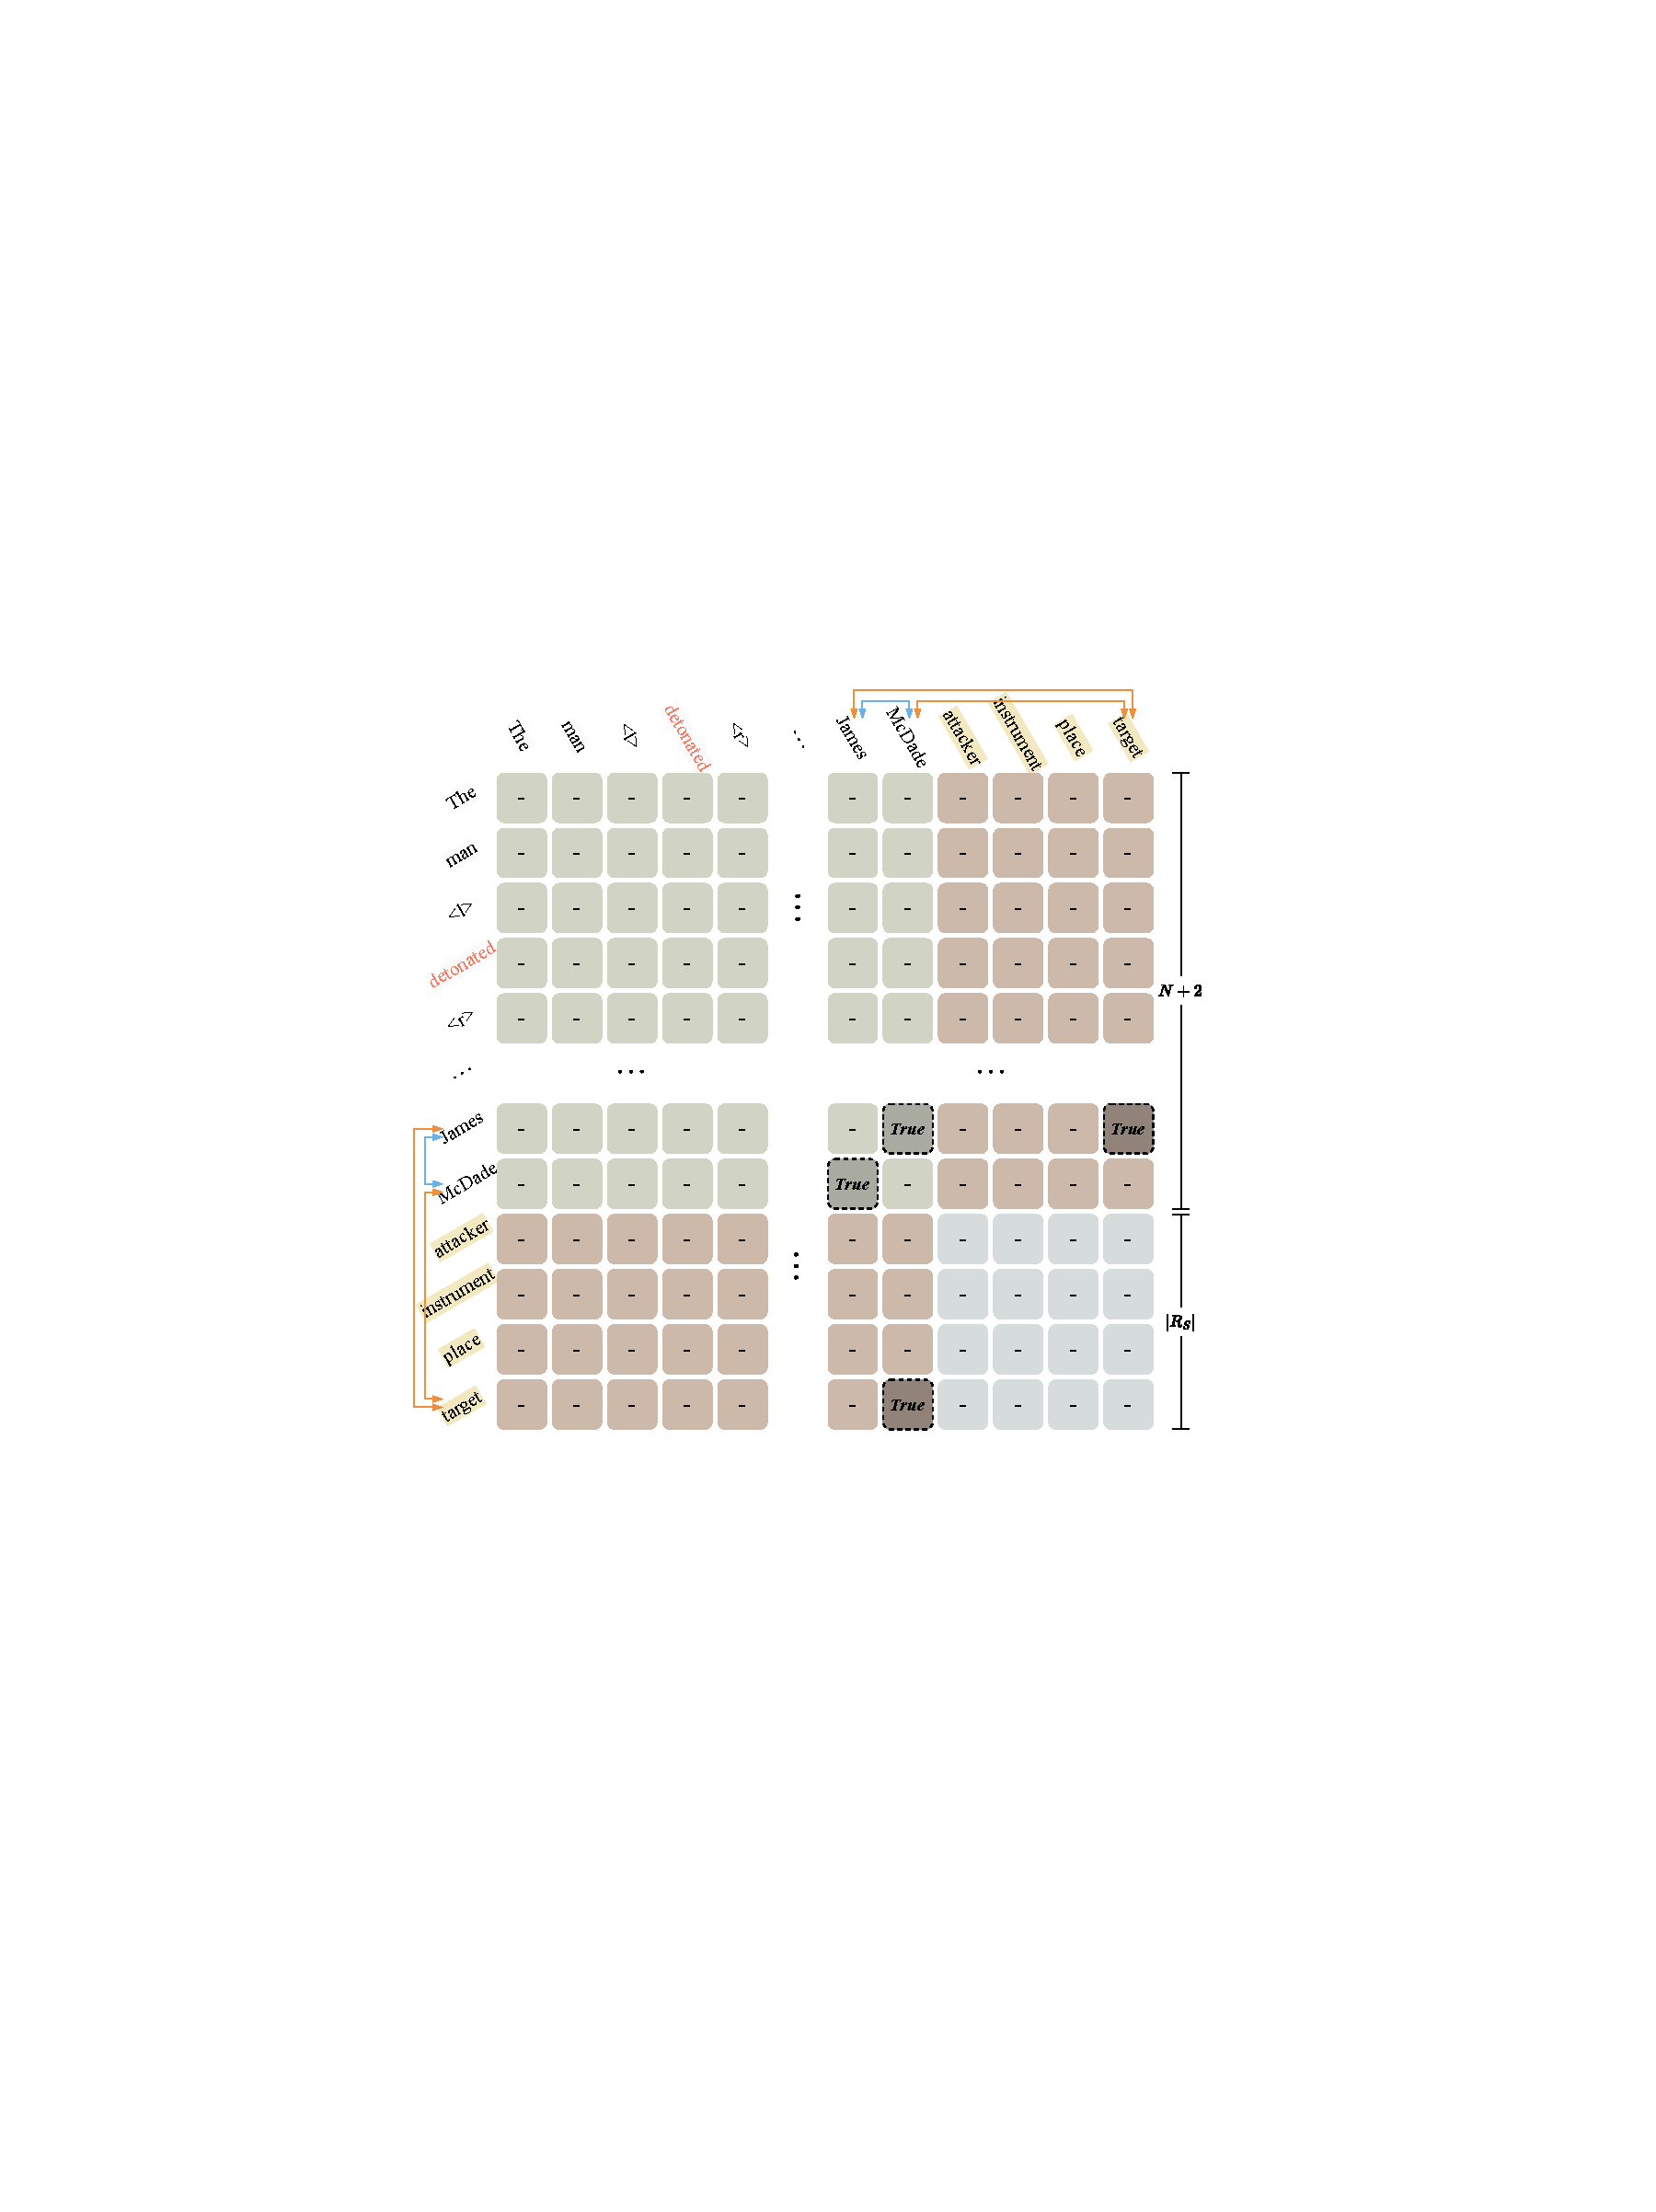
\includegraphics[width=0.6\linewidth]{figures/chap5/label_single_frame.pdf}
\caption{标签矩阵$\boldsymbol{L}_{S}$示例图}
\label{single_event_label}
\end{figure}

\textbf{得分矩阵}~与多事件链接构造模块中的公式\ref{scores}相同,本模块同样根据所使用的预训练语言模型的最后一层,利用其未通过softmax归一化的平均多头自注意权重作为多词元间的链接分数,表示为$\boldsymbol{A}_{S} \in {\mathbb{R}}^{(N+|R_{S}|+2) \times (N+|R_{S}|+2)}$。

\textbf{训练损失}~为了利用到获取的跨事件信息,首先采用两阶段融合模块(其将在下一模块中作详细介绍)来得到最终的词元链接预测矩阵:
\begin{equation}
\boldsymbol{P} =\textrm{TFF}(\boldsymbol{E}^{M},\boldsymbol{E}^{S},\boldsymbol{A}_{S})
\end{equation} 
其中$\textrm{TFF}$指两阶段融合模块。然后,可以得到训练损失$\mathcal{L_\textrm{EAE}}$如下:\begin{equation}
\label{binary}
\begin{split}
    \mathcal{L_\textrm{EAE}} = & -\frac{1}{(N+|R_{S}|+2)^2} \sum_i \sum_j\left(L^{S}_{i,j} \log {P}[i][j] + \right. \\
    & \left. (1-L^{S}_{i,j}) \log \left(1- {P}[i][j]\right) \right)
\end{split}
\end{equation} 
其中当${L}_{S}[i][j]$为“\emph{True}”时,设置
$L^{S}_{i,j}$为1,否则设置$L^{S}_{i,j}$为0。

\subsection{两阶段融合}
\label{two-fold}
本模块利用聚合了跨事件要素类型信息的文本表示来增强目标事件的要素抽取。具体地,首先动态融合来自上述两个链接模块的文本表示,即第一阶段融合。然后,使用融合的文本表示来获得目标事件的另一个词元链接得分矩阵,其不同于$\boldsymbol{A}_{S}$。这两个词元链接得分矩阵进一步被融合为最终的链接预测,即第二阶段融合。

\textbf{第一阶段融合}~由于$\boldsymbol{E}^{M}$中的文本向量涉及多事件信息,本模块首先利用条件层归一化(Conditional Layer Normalization,CLN)~\cite{yu2021semi,xu2022extracting}来获取与目标事件(触发词)相关的上下文向量。对于目标事件触发词$t$,本模块简单地将其输入到一个参数冻结的预训练语言模型中,并使用得到的第一个词元向量来表示该触发词,记作$\boldsymbol{t}$。然后,对于$\boldsymbol{E}^{M}$中的每个词元向量$\boldsymbol{h}_{n}^{M} \left(1 \leq n \leq N\right)$,可得到相应的向量$\boldsymbol{\hat{h}}_{n}^{M} \left(1 \leq n \leq N\right)$如下:
\begin{equation}
    \boldsymbol{\alpha}_{t}=\boldsymbol{t}\boldsymbol{W}_\alpha+\boldsymbol{b}_\alpha
\end{equation}
\begin{equation}
    \boldsymbol{\beta}_{t}=\boldsymbol{t}\boldsymbol{W}_\beta+\boldsymbol{b}_\beta
\end{equation}
\begin{equation}
    \boldsymbol{\hat{h}}_{n}^{M} = \textrm{CLN}(\boldsymbol{h}_{n}^{M}, \boldsymbol{\alpha}_{t}, \boldsymbol{\beta}_{t})=\boldsymbol{\alpha}_{t} \odot\left(\frac{\boldsymbol{h}_{n}^{M}-\mu}{\sigma}\right)+\boldsymbol{\beta}_{t}
\end{equation}
其中$\boldsymbol{W}_\alpha \in {\mathbb{R}}^{d_{1} \times d_{1}}$, $\boldsymbol{W}_\beta \in {\mathbb{R}}^{d_{1} \times d_{1}}$, $\boldsymbol{b}_\alpha \in {\mathbb{R}}^{d_{1}}$和$\boldsymbol{b}_\beta \in {\mathbb{R}}^{d_{1}}$为可训练的参数,$\mu$和$\sigma$分别为根据$\boldsymbol{h}_{n}^{M}$中的向量元素计算得到的平均值和标准偏差,$d_{1}$为向量$\boldsymbol{t}$的维度。然后,在$(\boldsymbol{\hat{h}}_{1}^{M}, \cdots, \boldsymbol{\hat{h}}_{N}^{M})$中插入零向量$\boldsymbol{0}$,以便与文本向量$\boldsymbol{E}^{S}$进行对齐:
\begin{equation}
(\boldsymbol{\bar{h}}_{1}^{M}, \cdots, \boldsymbol{\bar{h}}_{N+2}^{M}) = (\boldsymbol{\hat{h}}_{1}^{M}, \cdots, \boldsymbol{0}, \boldsymbol{\hat{h}}_{i}^{M}, \cdots, \boldsymbol{\hat{h}}_{j}^{M}, \boldsymbol{0}, \cdots, \boldsymbol{\hat{h}}_{N}^{M})
\end{equation} 
其中$i$和$j$对应于触发词$t$的词元向量在$(\boldsymbol{h}_{1}^{S}, \cdots, \boldsymbol{h}_{N+2}^{S})$中的开始和结束位置。最后,动态融合不同的文本向量。给定两个词元向量 $\boldsymbol{h}_{n}^{S}$和$\boldsymbol{\bar{h}}_{n}^{M}$ $(1 \leq n \leq N+2)$,本模块使用门控融合机制以获取词元向量$\boldsymbol{h}_{n}^{F}$:
\begin{equation}
\boldsymbol{g}_{n}=\sigma\left(\left[\boldsymbol{h}_{n}^{S}; \boldsymbol{\bar{h}}_{n}^{M}\right]\boldsymbol{W}_{G}\right)
\end{equation} 
\begin{equation}
\boldsymbol{h}_{n}^{F} = \boldsymbol{g}_{n} \odot \boldsymbol{h}_{n}^{S} + \left(1-\boldsymbol{g}_{n}\right) \odot \boldsymbol{\bar{h}}_{n}^{M}
\end{equation} 
其中$\sigma(\cdot)$为sigmoid函数,$\boldsymbol{W}_{G} \in {\mathbb{R}}^{2d_{1} \times d_{1}}$为可训练学习的矩阵,$\odot$表示元素依次相乘操作。

\textbf{第二阶段融合}~首先,串接融合的文本向量$(\boldsymbol{h}_{1}^{F}, \cdots, \boldsymbol{h}_{N+2}^{F})$和要素类型对应的词元向量$(\boldsymbol{r}_{1}^{S}, \cdots, \boldsymbol{r}_{|R_{S}|}^{S})$,表示为$\boldsymbol{F}$。然后,本模块计算另一个词元链接得分矩阵$\boldsymbol{A}_{F} \in {\mathbb{R}}^{(N+|R_{S}|+2) \times (N+|R_{S}|+2)}$如下:
\begin{equation}
\boldsymbol{F}_{Q}=\boldsymbol{F} \boldsymbol{W}_{Q},~\boldsymbol{F}_{K}=\boldsymbol{F} \boldsymbol{W}_{K}
\end{equation} 
\begin{equation}
    \boldsymbol{A}_{F}=\boldsymbol{F}_{Q} \boldsymbol{F}_{K}^\top
\end{equation}
其中$\boldsymbol{W}_{Q} \in {\mathbb{R}}^{d_{1} \times d_{2}}$和$\boldsymbol{W}_{K} \in {\mathbb{R}}^{d_{1} \times d_{2}}$为可训练学习的矩阵。最后,根据$\boldsymbol{A}_{F}$和章节\ref{target_event_module}中得到的得分矩阵$\boldsymbol{A}_{S}$,使用blending层~\cite{wolpert1992stacked}融合如下:
\begin{equation}
\boldsymbol{P}=\sigma (\boldsymbol{A}_{S} + \boldsymbol{A}_{F} - \tau)
\end{equation} 
其中$\tau$为可训练的参数。

\subsection{训练和推理}
\textbf{训练}~本章提出模型的整体训练损失可根据如下得到:  
\begin{equation}
 \mathcal{L} = \alpha \mathcal{L_\textrm{EAE}} + (1-\alpha) \mathcal{L_\textrm{TR}}
 \label{overall_loss}
\end{equation}
其中$\alpha\,(0 < \alpha < 1)$为权重参数。

\textbf{推理}~基于词元链接预测矩阵$\boldsymbol{P}$,对于其中的每一个链接对$(i,j)$,如果对应预测值${P}[i][j](1 \leq i,j \leq N+|R_{S}|+2)$超过设定的阈值参数$\delta$,则将该链接对添加到链接对集合$\mathcal{C}$中。然后,使用$\mathcal{C}$作为输入,运行如算法\ref{algorithm_arg}所示的推理算法,得到目标事件的要素集合$\mathcal{A}$。对于$\mathcal{A}$中的每个元素$(start, end, role)$,$start$和$end$分别表示要素的开始和结束位置,$role$为对应的要素类型在$R_{S}$中的索引。 

\begin{algorithm}[tb]
\caption{目标事件的要素推理}
\label{algorithm_arg}
\textbf{Input}: 预测的链接对集合$\mathcal{C}((s_{k},e_{k})), k \in (1,\cdots,|\mathcal{C}|)$.\\
\textbf{Output}: 事件要素集合$\mathcal{A}$.
\begin{algorithmic}[1] %[1] enables line numbers
\STATE $cand\_span=set()$.
\STATE $start2r\_dict=\{\}$,~$end2r\_dict=\{\}$.
\FOR{$(s_{k}, e_{k}) \in \mathcal{C}$}
\IF {$s_{k} \leq N+2$ \AND $e_{k} \leq N+2$}
\STATE 将元组$(s_{k},e_{k})$添加到集合$cand\_span$
\ELSIF{$s_{k} \leq N+2$ \AND $e_{k} > N+2$}
\STATE 将键值对$(s_{k},e_{k}-N-2)$添加到字典$start2r\_dict$
\ELSIF{$s_{k} > N+2$ \AND $e_{k} \leq N+2$}
\STATE 将键值对$(e_{k},s_{k}-N-2)$添加到字典
$end2r\_dict$
\ENDIF
\ENDFOR
\FOR{$(s, e) \in cand\_span$}
\FOR{$r \in (\textrm{set}(start2r\_dict[s])~\cap~\textrm{set}(end2r\_dict[e]))$}
\STATE 将元组$(s,e,r)$添加到集合$\mathcal{A}$
\ENDFOR
\FOR{$r \in (\textrm{set}(start2r\_dict[e])~\cap~\textrm{set}(end2r\_dict[s]))$}
\STATE 将元组$(e,s,r)$添加到集合$\mathcal{A}$
\ENDFOR
\ENDFOR
\end{algorithmic}
\end{algorithm}

\section{实验评估}
\label{section_5_3}
\subsection{实验设置}
\textbf{1.数据集}~为了评估所提模型,本章将在以下数据集上进行实验:
\begin{itemize}
\item ACE2005~\cite{doddington2004automatic} - 该数据集详细介绍见章节\ref{experiment_settings}。本章实验使用其事件标注数据进行句子级别事件要素抽取的评估。在数据预处理上,与章节\ref{settings_4}不同,本章遵循PAIE~\cite{ma2022prompt}和TabEAE~\cite{he2023revisiting}等通用事件要素抽取模型的设置,使用Du等人~\cite{du2020event}的预处理脚本。该脚本遵循DyGIE++~\cite{wadden2019entity}模型的设置。

\item RAMS~\cite{ebner2020multi} - 该文档级别事件要素抽取数据集来源于新闻文章。与原始数据集将同一上下文中的多个事件视为不同的实例不同,本章实验遵循TabEAE的预处理过程,聚合每个实例的同一上下文中出现的其他事件的标注信息。

\item WikiEvents~\cite{li2021document} - 该文档级别数据集来源英文维基百科。本章实验遵循PAIE的预处理程序,采用以每个目标事件触发词为中心的预定义窗口去截断过长的上下文内容,避免超出预训练语言模型的输入长度限制。

\item MLEE~\cite{pyysalo2012event} - 该文档级别事件要素抽取数据集基于生物医学领域的英文出版物摘要标注得到。在预处理方面,遵循TabEAE参照Trieu等人~\cite{trieu2020deepeventmine}的预处理设置。此外,由于MLEE数据集中不存在验证集,本章实验遵循TabEAE使用训练集调整模型的超参数。    
\end{itemize}

对于所有文档级别数据集,遵循He等人~\cite{he2023revisiting}设置预定义的窗口长度为250,将每个文档拆分为多个上下文片段。本章实验所用数据集的具体统计数据如表\ref{statistics}所示。

\begin{table}[htp]
\centering
\caption{数据集详细统计信息} 
% \emph{Avg Args} denotes the average number of arguments per event.
\begin{tabular}{l|cccc}
\toprule
 数据集 & ACE2005 & RAMS & WikiEvents & MLEE  \\
 \midrule
 \textbf{\#事件} &  &  &  &  \\
 训练集 & 4,202 & 7,329 & 3,241 & 4,442  \\
 验证集 & 450 & 924 & 345 & -  \\
 测试集 & 403 & 871 & 365 & 2,200  \\
 \midrule
 \textbf{\#事件要素} &  &  &  &  \\
 训练集 & 4,859 & 17,026 & 4,552 & 5,786 \\
 验证集 & 605 & 2,188 & 428 & - \\
 测试集 & 576 & 2,023 & 566  & 2,764 \\
 \midrule
 \textbf{\#事件类型} & 33 & 139 & 50 & 23  \\
 \textbf{\#要素类型} & 22 & 65 & 59 & 8 \\
 % \textbf{\#Avg Args} & 1.19 & 2.33 & 1.40 & 1.29  \\
\bottomrule
\end{tabular}
\label{statistics}
\end{table}

\textbf{2.评价指标}~
遵循之前通用文本级别事件要素抽取研究工作~\cite{ma2022prompt,he2023revisiting},本章采用两个指标来衡量模型性能。(1)要素识别F1得分(Argument Identification F1 score,Arg-I):当其事件要素文段的边界与事件中任意一个标注的要素相匹配,则认为该事件要素被正确识别。基于该识别准则,本章进一步计算对应的F1值评估要素识别性能,其F1值计算参照章节\ref{experiment_settings}。(2)要素分类F1得分(Argument Classification F1 score,Arg-C):当其事件要素文段的边界和要素类型都与事件中任意一个标注的要素相匹配,则认为该事件要素被正确分类。基于该分类准则,本章进一步计算对应的F1值评估要素分类性能,其F1值计算参照章节\ref{experiment_settings}。在实验中,使用三个不同的随机种子训练本章提出的Sep2F模型,并通过平均值计算得到相应的性能结果。

\textbf{3.实验配置}~
% \label{settings}
为了便于与最近的研究工作进行公平比较,本章实验在模型中使用RoBERTa-base和RoBERTa-large~\cite{liu2019roberta}作为预训练语言模型,其分别基于Huggingface上发布的“FacebookAI/roberta-base”文件\footnote{https://huggingface.co/FacebookAI/roberta-base}和“FacebookAI/roberta-large”文件\footnote{https://huggingface.co/FacebookAI/roberta-large}进行参数初始化。基于此两种模型,均采用配备了线性学习率调度器的Adam优化器和比率为0.1的warmup策略。$\delta$为等式\ref{binary}中二分类预测值${P}[i][j]$的推断阈值,因此实验中遵循常规的二分类设置,在所有数据集上均设置$\delta$为0.5。在RAMS数据集上设置训练轮次为50,在其他数据集上设置训练轮次为100。在ACE2005数据集上设置批数据大小为16,在其他数据集上设置批数据大小为8。对于ACE2005,$d_{2}$设置为32,而在其他数据集上$d_{2}$设置为64。此外,基于每个数据集的验证集,使用网格搜索调整各自模型的学习率和训练权重$\alpha$。具体地,在区间$\{0.5,~0.6,~0.7,~0.8,~0.9\}$内调整权重$\alpha$,在区间$\{3,~4,~5\} \times 10^{-5}$和$\{1,~2,~3\} \times 10^{-5}$内分别搜索基于RoBERTa-base和RoBERTa-large的模型的最佳学习率。表\ref{hyperparameter}列出了在不同数据集上最终选择的训练权重和学习率,其中表格上半部分为基于RoBERTa-base的模型的参数详情,表格下半部分为基于RoBERTa-large的模型的参数详情。对于基于RoBERTa-base的模型,不同数据集上的训练均在相同实验服务器上完成,具体配置为:CPU型号Intel(R) Xeon(R) Gold 5320,主频2.20GHz;内存256G;GPU计算卡型号NVIDIA GeForce RTX 3090,显存24G。对于基于RoBERTa-large的模型,其具体配置为:CPU型号Intel(R) Xeon(R) Silver 4314,主频2.40GHz;内存128G;GPU计算卡型号NVIDIA A100 PCIE,显存40G。本章实验均基于Pytorch~\cite{paszke2017automatic}框架完成。

\begin{table}[htp]
\centering
\caption{超参数设置}
\begin{tabular}{cccccc}
\toprule
超参数 & ACE2005 & RAMS & WikiEvents & MLEE  \\
 \midrule
 学习率 & 3e-5 & 5e-5 & 4e-5 & 4e-5  \\
 权重$\alpha$ & 0.7 & 0.7 & 0.8 & 0.6  \\
\midrule
 学习率 & 2e-5 & 3e-5 & 2e-5 & 1e-5  \\
 权重$\alpha$ & 0.8 & 0.5 & 0.7 & 0.8  \\
 \bottomrule
\end{tabular}
\label{hyperparameter}
\end{table}

\textbf{4.基线模型}~本章选择以下模型作为与所提的Sep2F模型进行实验比较的基线,其均在\textbf{句子级别和文档级别数据集}上评估了事件要素抽取任务的性能:
\begin{itemize}

\item EEQA~\cite{du2020event} - 该模型将事件要素抽取任务转化为机器阅读理解问题进行解决。
\item BART-Gen~\cite{li2021document} - 该模型将事件要素抽取建模为基于提示模版的条件生成任务。
\item PAIE~\cite{ma2022prompt} - 该模型提出了抽取式的提示学习方法,其利用要素类型对应的槽位表示查询对应的要素文段。
\item APE(Single)~\cite{zhang2023overlap} - 该模型通过将提示模版中的要素类型映射至对应的实体类型,实现了跨事件共享知识的学习。
\item PGAD~\cite{luo2023context} - 该模型引入了扩散模型,以获取多样化的上下文感知提示表示。
\item EDGE~\cite{li2023intra} - 该模型同时设计了事件内和跨事件的图,以丰富要素类型语义信息。
\item TabEAE~\cite{he2023revisiting} - 该模型将多事件要素抽取转换为表格生成,以捕捉事件间的关联。

\end{itemize}

最近,基于情境学习(In-Context Learning,ICL)~\cite{brown2020language}的ChatGPT在各种自然语言处理任务中表现出色。但是,目前缺乏对不同事件要素抽取数据集的全面评估,尤其是文档级别数据集。因此,本章按照Han等人~\cite{han2023information}的设置,构建5-shot ICL提示模版作为每个测试样本的输入,并使用OpenAI接口\footnote{https://platform.openai.com/}获取事件要素抽取的结果。具体地,本章使用两个版本的ChatGPT评估事件要素抽取的性能:\emph{gpt-3.5-turbo}和\emph{gpt-4},其分别由gpt-3.5和gpt-4模型构建。

此外,UnifiedEAE~\cite{zhou2022multi}和 APE~\cite{zhang2023overlap}等研究工作同时利用了多个数据集提升目标数据集的性能,以受益于额外的数据资源。因此,本章未将其作为主实验结果的比较基线,而是另作单独的分析。

\subsection{性能结果}
表\ref{overall}展示了在四个数据集上的事件要素抽取实验结果,其中粗体表示在各自数据集上的最优性能,下划线表示在各自数据集上的次优性能结果,预训练模型所在列中的“b”和“l”分别表示对应的为base版本和large版本。从表\ref{overall}中可以观察到,本章提出的基于RoBERTa-large的模型在所有数据集上都取得了当前最优的性能。具体地,与之前性能最优的TabEAE模型相比,其在ACE2005、RAMS、 WikiEvent和MLEE数据集上,
分别在Arg-I/Arg-C F1指标上取得了\textbf{1.6\%/2.0\%}、\textbf{1.4\%/1.0\%}、 \textbf{2.6\%/2.8\%}和\textbf{2.4\%/2.5\%}的性能提升。而相比于使用了base版本预训练模型的最优基线,本章提出的基于RoBERTa-base的模型在ACE2005、RAMS和WikiEvent数据集上分别在Arg-I/Arg-C F1指标上取得了0.9\%/2.9\%、1.4\%/2.4\%和3.7\%/4.1\%的性能提升。此外,本章所提的base模型在WikiEvents和MLEE数据集上超越了所有使用large版本预训练模型的基线,且在ACE2005和RAMS数据集上相比large基线模型也展现了具有竞争力的性能。因此,可以得知本章提出的Sep2F模型在处理不同文本级别的事件要素抽取任务时均表现出色。

\begin{table*}[htp]
\centering
\small
\caption{四种数据集上的事件要素抽取性能结果}
% The best score is in bold and the second best score is underlined. b and l in the column PLM represent the base and large models, respectively. Note that we report the averaged results of our Sep2F with three different fixed random seeds.}
\begin{tabular}{llcccccccc}
\toprule
\multicolumn{1}{l}{\multirow{2}{*}{模型}} & \multicolumn{1}{l}{\multirow{2}{*}{预训练模型}} & \multicolumn{2}{c}{ACE2005} & \multicolumn{2}{c}{RAMS} & \multicolumn{2}{c}{WikiEvents} & \multicolumn{2}{c}{MLEE} \\ \cmidrule(lr){3-4} \cmidrule(lr){5-6} \cmidrule(lr){7-8} \cmidrule(lr){9-10}
\multicolumn{1}{l}{}                       & \multicolumn{1}{l}{}                     & Arg-I        & Arg-C        & Arg-I       & Arg-C      & Arg-I          & Arg-C         & Arg-I       & Arg-C      \\ \midrule
\multicolumn{1}{l}{ChatGPT}   & \multicolumn{1}{l}{GPT-3.5} & 35.6 & 30.0 & 25.1 & 19.3 & 13.6 & 11.6 &  15.7 & 11.8  \\
\multicolumn{1}{l}{ChatGPT}   & \multicolumn{1}{l}{GPT-4}  & 37.5 & 33.2 & 23.8 & 20.9 & 16.7 & 15.3 & 16.9 & 14.9 \\ \midrule
\multicolumn{1}{l}{BART-Gen}  & \multicolumn{1}{l}{BART-b} & 59.6 & 55.0 & 50.9 & 44.9 & 47.5 & 41.7 & - & - \\
\multicolumn{1}{l}{PAIE}  & \multicolumn{1}{l}{BART-b} 
& 73.6 & 69.8 & 54.7 & 49.5 & 68.9 & 63.4 & - & - \\
\multicolumn{1}{l}{APE(Single)}  & \multicolumn{1}{l}{BART-b} & 74.1 & 70.1 & 54.8 & 49.6 & 66.2 & 62.1 & - & - \\
\multicolumn{1}{l}{PGAD}  & \multicolumn{1}{l}{BART-b} & 74.1 & 70.5 & 53.7 & 45.9 & 69.6 & 64.1 & - & - \\
\multicolumn{1}{l}{EDGE}  & \multicolumn{1}{l}{BART-b} & 75.3 & 70.6 & 55.2 & 49.7 & 68.2 & 62.8 & - & - \\ 
\multicolumn{1}{l}{\textbf{Sep2F}}   & \multicolumn{1}{l}{RoBERTa-b}  & 76.2 & 73.5 & 56.6 & 52.1 & \underline{73.3} & \underline{68.2} & \underline{76.8} & \underline{75.6} \\ \midrule

\multicolumn{1}{l}{EEQA}  & \multicolumn{1}{l}{RoBERTa-l}   & 72.1 & 70.4 & 51.9 & 47.5 & 60.4 & 57.2 & 70.3 & 68.7 \\  
\multicolumn{1}{l}{BART-Gen}  & \multicolumn{1}{l}{BART-l}   & 69.9 & 66.7 & 51.2 & 47.1 & 66.8 & 62.4 & 71.0 & 69.8 \\
\multicolumn{1}{l}{PAIE}  & \multicolumn{1}{l}{BART-l} 
& 75.7 & 72.7 & 56.8 & 52.2 & 70.5 & 65.3 & 72.1 & 70.8 \\
\multicolumn{1}{l}{PAIE}  & \multicolumn{1}{l}{RoBERTa-l}   & 76.1 & 73.0 & 57.1 & 52.3 & 70.9 & 65.5 & 72.5 & 71.4 \\
\multicolumn{1}{l}{APE(Single)}  & \multicolumn{1}{l}{BART-l} & 75.3 & 72.9 & 56.3 & 51.7 & 70.6 & 65.8 & - & - \\
\multicolumn{1}{l}{TabEAE}  & \multicolumn{1}{l}{RoBERTa-l}
& \underline{77.2} & \underline{75.0} & \underline{57.3} & \underline{52.7} & 71.4 & 66.5 & 75.1 & 74.2 \\
\multicolumn{1}{l}{\textbf{Sep2F}}   & \multicolumn{1}{l}{RoBERTa-l}  & \textbf{78.8} & \textbf{77.0} & \textbf{58.7} & \textbf{53.7} & \textbf{74.0} & \textbf{69.3} & \textbf{77.5} & \textbf{76.7} \\
% \midrule
% \multicolumn{10}{c}{+Extra training datasets} \\
% \midrule
% \multicolumn{1}{l|}{UnifiedEAE~(\citeyear{zhou2022multi})}   & \multicolumn{1}{l|}{BART-b} & 76.1 & 71.9 & 55.5 & 49.9 & 69.8 & 64.0 & - & - \\
% \multicolumn{1}{l|}{APE~(\citeyear{zhang2023overlap})}   & \multicolumn{1}{l|}{BART-b} & 75.5 & 72.9 & 56.1 & 51.6 & 70.7 & 66.0 & - & - \\
% \multicolumn{1}{l|}{APE~(\citeyear{zhang2023overlap})}   & \multicolumn{1}{l|}{BART-l} & 
% 78.2 & 75.4 & 58.1 & 54.3 & 73.7 & 68.7 & - & - \\
\bottomrule
\end{tabular}
\label{overall}
\end{table*}

另外,可以观察到不同版本的ChatGPT在事件要素抽取任务上的性能都明显落后于当前有监督模型。尤其在处理更具挑战性的文档级别事件要素抽取任务时,性能差距通常会进一步扩大。因此,提升ChatGPT等大语言模型在事件要素抽取任务上的性能表现仍有待深入探索研究。

\subsection{不同多词元链接模型性能比较}

如章节\ref{introduction}中所述,基于多词元链接操作的现有事件要素抽取模型主要存在两种方式:单事件抽取和多事件抽取。然而,这些方法将事件要素抽取任务作为端到端的通用信息抽取或事件抽取中的一个子任务进行建模。因此,其实验设置和训练数据集与单独处理事件要素抽取任务存在差异。为了更加公平地比较不同的多词元链接模型的性能,本章根据这些多词元链接模型的建模方式设计以下变体模型:(1)\textbf{SingleE} 在目标事件链接构造模块中移除两阶段融合,以抽取单个事件的要素信息,对应于单事件抽取方式。(2)\textbf{$\textrm{SingleE-L}$} 在模型输入中串接给定数据集的所有预定义要素类型名称与待抽取文本,其他设置与SingleE相同。(3)\textbf{MultiE} 同时抽取文本中多个事件的事件要素,对应多事件抽取方式。具体地,将事件要素抽取转化为多个<事件触发词,要素类型,要素文段>三元组抽取问题,并参照Tang等人在UniRel~\cite{tang2022unirel}模型中基于多词元组成的实体进行关系三元组抽取的代码实现\footnote{https://github.com/wtangdev/UniRel}。由于本章实验在事件要素抽取中使用正确标注的事件触发词作为输入,MultiE将在推理过程中根据标注信息纠正事件触发词的文段范围预测错误。此外,与MultiE输入文本串接的为只在待抽取事件中出现的要素类型名称。(4)\textbf{$\textrm{MultiE-L}$}将所有预定义的要素类型名称与待抽取文本串接,其他设置与MultiE相同。

\begin{table}[htp]
\centering
\caption{四种数据集上不同多词元链接模型在Arg-C F1(\%)指标上的结果对比}
\begin{tabular}{lcccc}
\toprule
\multicolumn{1}{l}{\multirow{2}{*}{模型}} & ACE2005 & RAMS & WikiEvents & MLEE \\ 
\multicolumn{1}{l}{} & [1.35] & [1.25] & [1.78] & [3.32] \\ \midrule
SingleE  & 75.4 & 53.0 & 66.5 & 74.4 \\
SingleE-L  & 72.9 & 49.1 & 55.8 & 73.0 \\
MultiE  & 69.9 & 49.3 & 47.9 & 57.2\\ 
MultiE-L & 68.1 & 40.5 & 26.5 & 8.4\\
Sep2F & \textbf{77.0} & \textbf{53.7} & \textbf{69.3} & \textbf{76.7} \\ 
% ratio & 6/22 & 5/65 & 6/59 & 4/14 \\
\bottomrule
\end{tabular}
\label{strategy}
\end{table}

表\ref{strategy}为上述的多词元链接模型在四个数据集上关于Arg-C F1(\%)指标的实验结果,其均使用RoBERTa-large进行编码,且“$[\cdot]$”表示每个对应数据集中单个数据实例存在的平均事件数目。首先,从表\ref{strategy}中可以总结出本章提出的模型在四个数据集上的性能均超越了所有变体模型。接下来,给出详细比较如下:

\begin{itemize}
\item SingleE vs Sep2F:与本章提出的Sep2F模型相比,未利用跨事件信息的SingleE的Arg-C F1指标在ACE2005、RAMS、WikiEvents和MLEE数据集上分别下降了1.6\%、0.7\%、2.8\%和2.3\%。
\item MultiE vs Sep2F:MultiE在事件要素抽取任务上未表现出有竞争力的性能,尤其是在WikiEvents和MLEE数据集上,MultiE和本章所提的Sep2F的性能存在显著差距。
\item SingleE vs SingleE-L:在不同数据集上SingleE-L的Arg-C F1指标均低于SingleE,其验证了在文本和要素类型名称间进行链接预测时,串接更多的要素类型会降低预测的性能。此外,图\ref{relevance}进一步展示了这两个模型在不同数据集上要素类型串接长度和Arg-C F1指标的关联性,其中“增加的要素类型长度”表示SingleE-L输入中拼接的要素类型序列相比于SingleE输入中拼接的最长要素类型序列增加了的长度,“Arg-C F1下降值”表示SingleE和SingleE-L的性能差距。根据图\ref{relevance}可以观察到,由于SingleE-L与SingleE在RAMS和WikiEvents数据集上的要素类型串联比其他数据集更长,导致其在这两个数据集上的Arg-C F1指标差异也会相应地更加显著。
\item MultiE vs MultiE-L:与SingleE和SingleE-L的比较结果相比,MultiE和MultiE-L的性能差距进一步增加,其增加程度和不同数据集上单个数据实例的平均事件数目密切相关。例如,MLEE数据集上单个数据实例的平均事件数超过三个,导致MultiE-L性能的大幅下降。
\item SingleE-L vs MultiE-L: 尽管MultiE-L模型同时抽取多个事件的事件要素,以便考虑不同事件间的关联性。但是,当MultiE-L和SingleE-L保持相同的要素类型串接时,其Arg-C F1指标在所有数据集上均低于SingleE-L模型。此结果表明,MultiE-L无法高效地在单个数据实例中处理更多的词元链接预测。因此,其跨事件信息带来的性能提升未能弥补更多累积错误导致的性能下降。此外,WikiEvents和MLEE数据集上单个实例的平均事件数量相比其他数据集较多,导致在这两个数据集上SingleE-L和MultiE-L的性能差异更大。
\end{itemize}

\begin{figure}[htp]
\centering
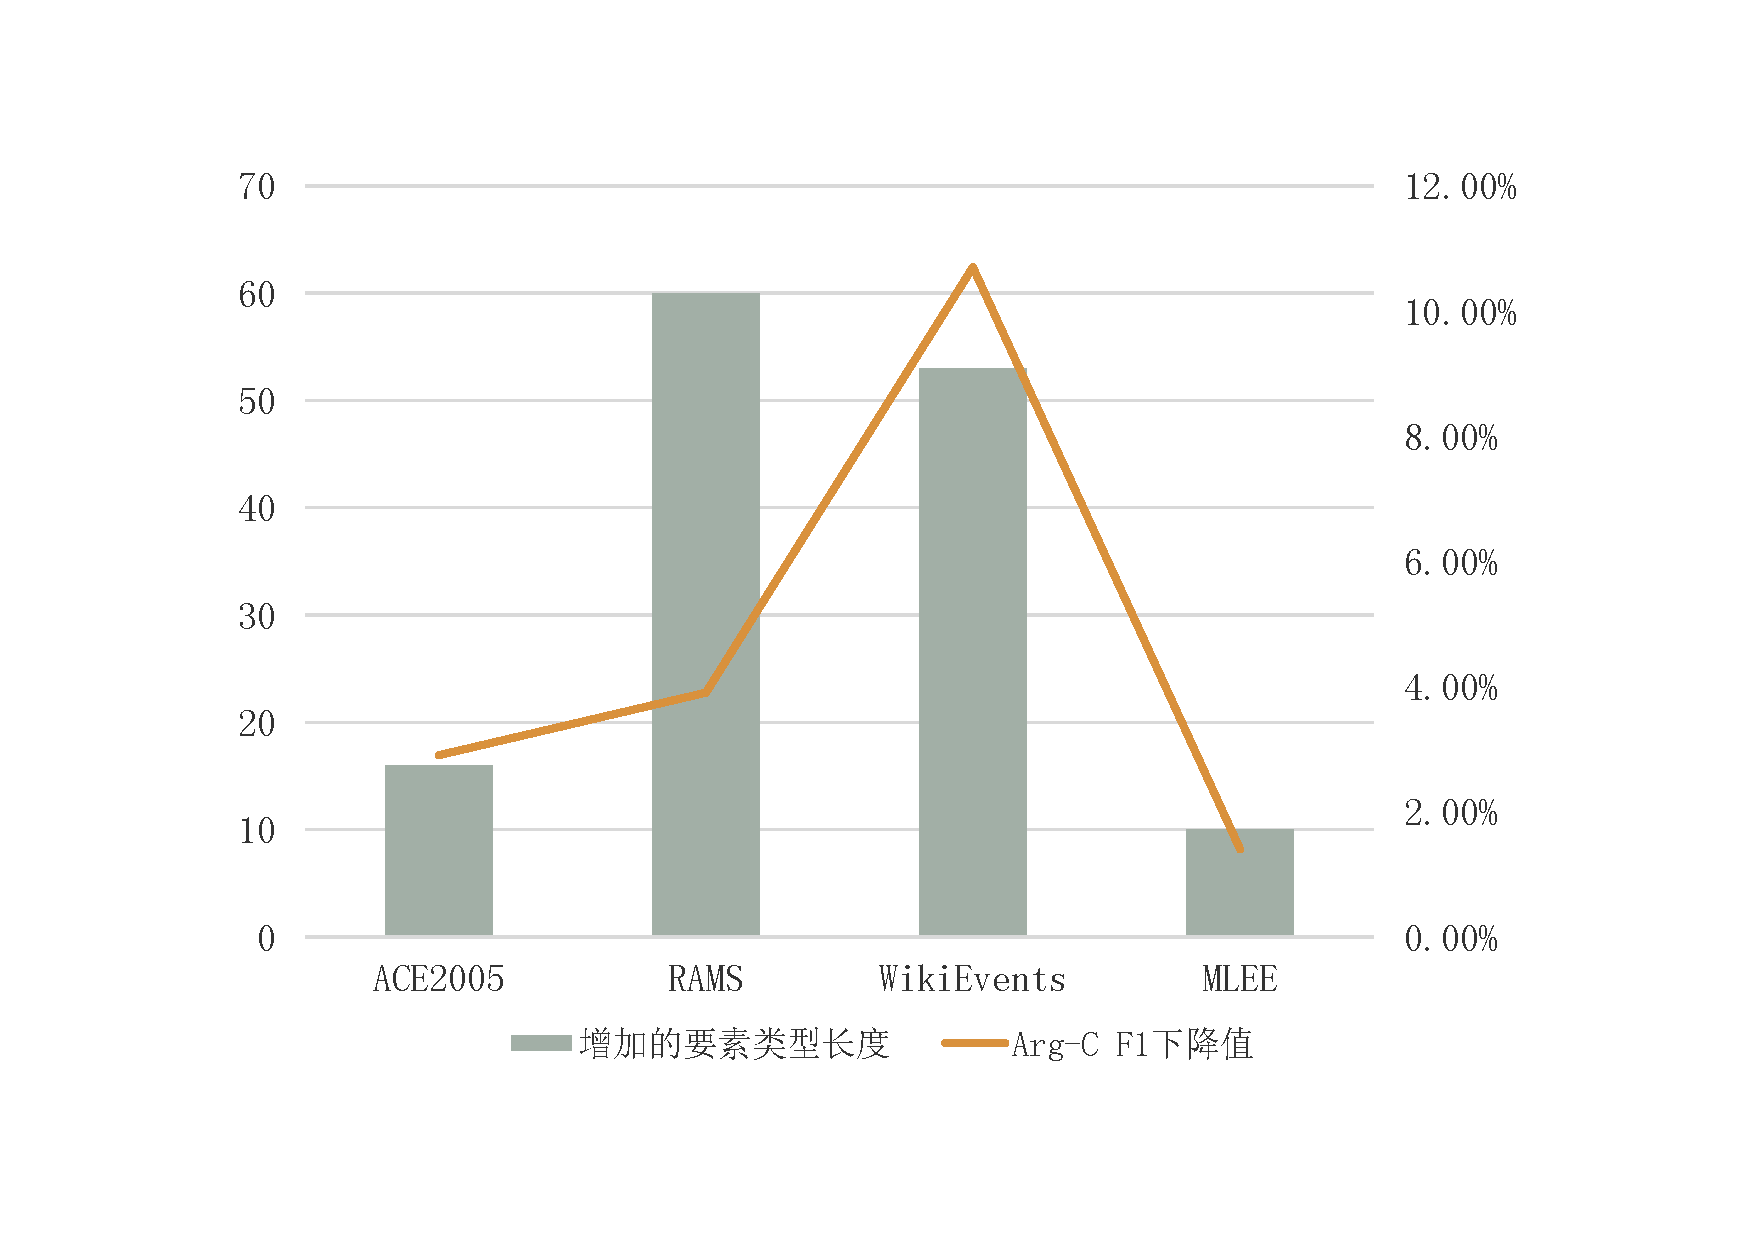
\includegraphics[width=0.55\linewidth]{figures/chap5/relevance.pdf}
\caption{要素类型串接长度与Arg-C F1指标的关联性}
\label{relevance}
\end{figure}

\subsection{单事件/多事件实例性能分析}遵循He等人~\cite{he2023revisiting}的实验设置,本节根据目标抽取事件所在上下文中存在的其他事件的数量(即$|C|$),将每个数据集的测试实例分为两组。当$|C|=0$时,实例中只存在目标抽取事件。如果$|C|>0$,则实例中存在多个事件。然后,基于分组得到各自的统计和性能信息如表\ref{multisingle}所示,其中$[\cdot]$中的值表示对应分组中测试实例的数量,Sep2F-b和Sep2F-l分别表示基于RoBERTa-base和RoBERTa-large的Sep2F模型。值得注意的是,表中其他的基线模型均基于RoBERTa-large进行构建。从表\ref{multisingle}中可以观察到:(1)在两个分组中,基于RoBERTa-large的Sep2F模型在Arg-C F1指标上均超越了之前性能最优的基线。这种性能的提升可以归因于本章所提的分离-融合范式,其同时保留了单事件抽取方式和多事件抽取方式的优点。(2)基于RoBERTa-base的Sep2F模型在WikiEvents和MLEE数据集包含多个事件的实例分组上表现出了令人印象深刻的性能结果,其超越了两个最具性能竞争力的基于RoBERTa-large的SingleE和TabEAE。这验证了本章提出的模型在处理具有多个事件的实例时的良好表现。(3)尽管SingleE和PAIE模型均未利用到跨事件信息,但与PAIE相比,SingleE在所有数据集上均表现出更好的性能结果,其验证了基于多词元链接的模型解决事件要素抽取任务的潜力和优势。

\begin{table*}[htp]
\small
\centering
\caption{四种数据集上单事件/多事件实例对应的Arg-C F1(\%)指标结果}
\begin{tabular}{llcccccccc}
\toprule
\multicolumn{1}{l}{\multirow{3}{*}{模型}} & \multicolumn{2}{c}{ACE2005} & \multicolumn{2}{c}{RAMS} & \multicolumn{2}{c}{WikiEvents} & \multicolumn{2}{c}{MLEE} \\ \cmidrule(lr){2-3} \cmidrule(lr){4-5} \cmidrule(lr){6-7} \cmidrule(lr){8-9}
\multicolumn{1}{l}{} & $|C|=0$ & $|C|>0$ & $|C|=0$ & $|C|>0$ & $|C|=0$ & $|C|>0$  & $|C|=0$  & $|C|>0$ \\ 
\multicolumn{1}{l}{} & [185] & [218] & [587] & [284] & [114] &  [251] &  [175] &  [2025]  \\ \midrule
\multicolumn{1}{l}{SingleE} & 74.8 & 76.0 & 52.9 & 53.3 & 68.4 & 65.5 & 83.1 & 73.8 \\
\multicolumn{1}{l}{MultiE}  & 70.8 & 69.1 & 50.0 & 47.5 & 45.5 & 49.1 & 53.7 & 57.5 \\
\multicolumn{1}{l}{PAIE}  & 71.0 & 73.9 & 52.7 & 52.1 & 65.3 & 65.4 & 78.9 & 70.1 \\
\multicolumn{1}{l}{TabEAE} & 73.4 & 76.1 & 52.9 &  52.5 & 67.3 &  66.2 & 81.1 & 73.6 \\
\midrule
\multicolumn{1}{l}{\textbf{Sep2F-b}} & 72.8 & 74.0 & 52.1 & 52.0 & 66.8 & 69.0 & \textbf{85.5} & 74.9 \\
\multicolumn{1}{l}{\textbf{Sep2F-l}} & \textbf{75.4} & \textbf{78.3} & \textbf{53.2} & \textbf{54.6} & \textbf{68.8} & \textbf{69.5} & 84.3 & \textbf{76.1} \\
\bottomrule
\end{tabular}
\label{multisingle}
\end{table*}

\subsection{消融研究}
本章通过消融研究分析基于RoBERTa-large的Sep2F模型中不同组件的有效性,包括第一阶段融合(First-fold Fusion)、第二阶段融合(Second-fold Fusion)、Blending层(Blending Layer)、文本中存在的其他事件信息(Surrounding Events $C$)和训练损失$\mathcal{L_\textrm{TR}}$(Training Loss $\mathcal{L_\textrm{TR}}$)。根据表\ref{ablation-Sep2F}所示的在Arg-C F1(\%)指标上的消融结果,所有组件均能提升本章提出的Sep2F模型的性能。具体地,可以观察到:(1)如果移除第一阶段融合或第二阶段融合,Sep2F模型在各个数据集上的性能均将下降。这表明两个阶段的融合均对性能提升贡献显著。(2)移除两个阶段中任意一阶段的融合,Sep2F模型在各个数据集上,尤其是WikiEvents和MLEE数据集,取得与之前性能表现最优的事件要素抽取基线模型相当的Arg-C F1指标。这展现了本章提出的模型即使利用简单的融合方法,仍然能在事件要素抽取任务上表现良好,进一步验证了分离-融合范式的优势。(3)当移除Blending层并直接对两个词元链接得分矩阵进行加和,Sep2F模型的Arg-C F1指标在所有数据集上均下降了1.0\%以上,这表明Blending层可以较好地集成不同的词元链接预测分数。(4)如果移除给定目标事件上下文中的其他事件$C$,并在多事件链接构建模块中保留目标事件触发词和在该事件中出现的要素类型之间的链接,则可以发现Sep2F模型在所有数据集上的性能均出现下降,从而明确地证明了跨事件依赖信息对于模型的性能增益。此外,可以发现Sep2F模型在ACE2005和RAMS数据集上性能略有下降,而在WikiEvents和MLEE数据集上则性能下降的更加显著。该观察结果可以归因于表\ref{strategy}中展示的各个数据集中单个实例的平均事件数目的差异。与ACE2005和RAMS数据集相比,本章提出的模型可以利用到WikiEvents和MLEE数据集上更多事件的跨事件信息。因此,与其他两个数据集相比,移除目标事件周围的其他事件信息会导致Sep2F模型在WikiEvents和MLEE数据集上更显著的性能下降。(5)如果移除多事件链接构造模块中的训练损失$\mathcal{L_\textrm{TR}}$(即设置公式\ref{overall_loss}中的训练权重参数$\alpha$为1),则意味着Sep2F模型无法通过调整$\mathcal{L_\textrm{TR}}$而利用到上下文中其他事件的要素类型信息。从消融结果可以看出,由此丢失的跨事件信息使得模型的Arg-C F1指标在ACE2005、RAMS、WikiEvents和MLEE数据集上分别下降了1.2\%、1.8\%、2.3\%和1.9\%。

\begin{table}[htp]
\centering
\caption{四种数据集上关于Arg-C F1(\%)指标的消融研究结果}
\begin{tabular}{lcccc}
\toprule
模型 & ACE2005 & RAMS & WikiEvents & MLEE \\ \midrule
% Sep2F & 73.5 & 52.1 & 68.2 & 75.6 \\ \midrule
% - First-fold Fusion  & 71.5 & 51.3 & 66.1 & 74.0 \\
% - Second-fold Fusion  & 69.6 & 49.7 & 64.3 & 73.9 \\ \midrule
Sep2F & 77.0 & 53.7 & 69.3 & 76.7 \\ \midrule
- First-fold Fusion  & 74.8 & 51.2 & 66.3 & 75.6 \\
- Second-fold Fusion  & 72.5 & 50.2 & 67.8 & 74.2 \\
- Blending Layer  & 75.9 & 52.2 & 66.6 & 75.9 \\
- Surrounding Events $C$  & 76.5 & 52.6 & 66.2 & 74.3 \\
- Training Loss $\mathcal{L_\textrm{TR}}$ & 75.8 & 51.9 & 67.0 & 74.8 \\
\bottomrule
\end{tabular}
\label{ablation-Sep2F}
\end{table}

\subsection{与资源增强模型的性能比较}
本章将Sep2F模型与聚焦于利用跨数据集知识的UnifiedEAE和APE模型作比较,其中APE还额外人工构建了学习重叠知识的提示模版。图\ref{cross-dataset}展示了性能比较结果,其中上半部分的图展示的为基于base版本预训练语言模型的比较,而下半部分的图展示的为基于large版本预训练语言模型的结果。在使用base版本的预训练语言模型时,本章提出的Sep2F模型在所有三个数据集上均优于UnifiedEAE和APE模型。此外,当使用large版本预训练模型时,Sep2F模型在ACE2005和WikiEvents数据集上的性能均优于APE,并在RAMS数据集上也取得与APE相当的Arg-C F1指标。因此,可以得知尽管参与比较的基线受益于额外的训练资源和人为设计的经验知识,本章提出的模型在使用不同版本预训练语言模型时仍能在绝大部分数据集上实现最佳性能,进一步证明了其在事件要素抽取任务上的优越性。

\begin{figure}[htp]
\centering
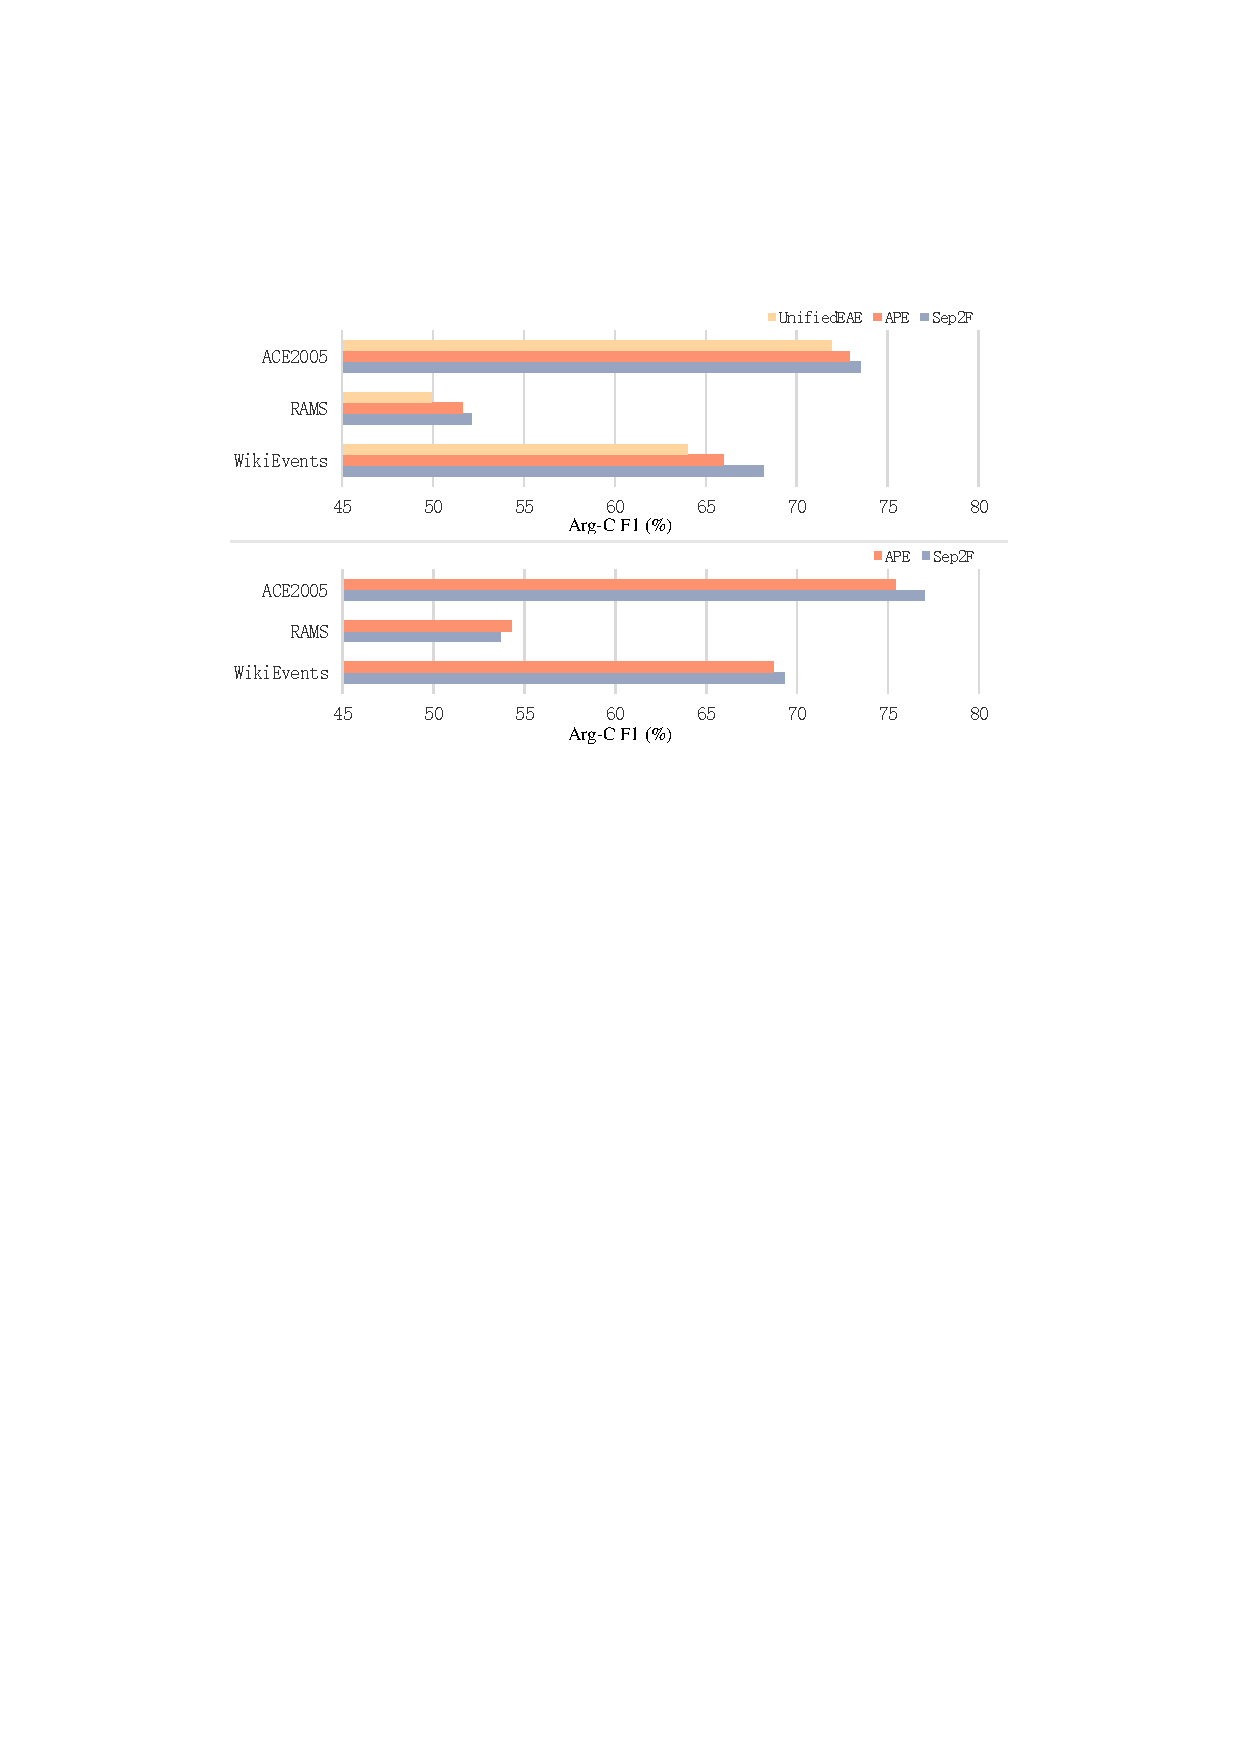
\includegraphics[width=1\linewidth]{figures/chap5/comparison.pdf}
\caption{三种数据集上Sep2F与资源增强模型的性能结果对比} 
% The upper figure illustrates the comparison using base-version PLMs, while the bottom figure shows the results with large-version PLMs.}
\label{cross-dataset}
\end{figure}

\subsection{案例研究}
本章节基于WikiEvents数据集中的一个具体实例进行定性的案例分析。图\ref{case-sep2f}展示了本章提出的Sep2F模型和SingleE模型在该实例上的事件要素抽取结果,其不同事件的触发词被不同颜色标记,且这两个模型均基于RoBERTa-large进行构建和训练。可以观察到,SingleE模型未能预测出由“booming”触发的$Attack$事件中的两个事件要素,但Sep2F模型给出了正确的预测结果。本章推测其原因为Sep2F模型可以利用到由“killed”触发的事件中的要素类型信息。同样,由于跨事件要素类型$Destroyer$提供了重要的依赖信息提示,Sep2F模型避免了事件触发词“death”的干扰,将“He”的要素类型识别为$Killer$而不是$Victim$,但SingleE模型给出了错误的抽取结果。

\begin{figure}[htp]
\centering
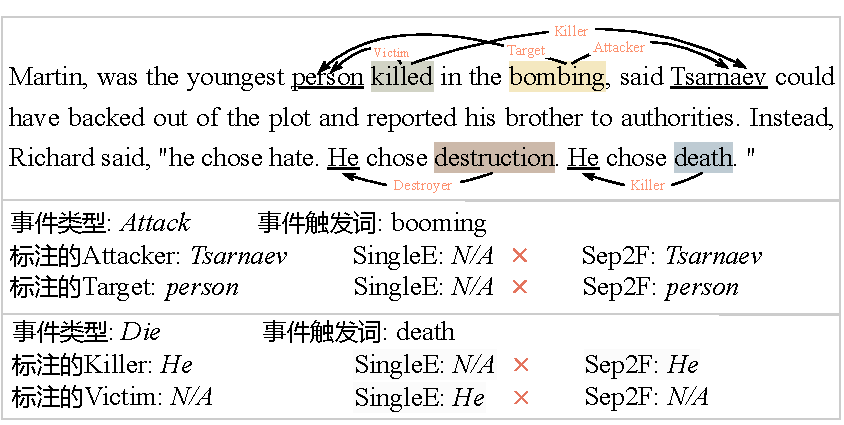
\includegraphics[width=0.8\linewidth]{figures/chap5/case-sep2f.pdf}
\caption{WikiEvents数据集上的案例分析}
\label{case-sep2f}
\end{figure}

\subsection{训练权重超参数分析}
本章研究公式\ref{overall_loss}中训练权重$\alpha$对于Sep2F模型性能的影响。表\ref{alpha_Sep2F}展示了不同$\alpha$取值下Sep2F模型在各个数据集上的Arg-C F1性能指标,可以观察到本章提出的Sep2F模型在不同数据集上均性能稳定,证明了其良好的鲁棒性。

\begin{table}[htp]
\centering
\caption{四种数据集上不同$\alpha$取值对应的Arg-C F1(\%)指标结果}
\begin{tabular}{ccccc}
\toprule
训练权重$\alpha$ & ACE2005 & RAMS & WikiEvents & MLEE \\ \midrule
0.5  & 76.1 & \textbf{53.7} & 68.6 & 76.6 \\
0.6  & 76.8 & 53.0 & 68.7 & 76.4 \\
0.7  & 76.7 & 53.1 & \textbf{69.3} & 76.6 \\
0.8  & \textbf{77.0} & 52.7 & \textbf{69.3} & \textbf{76.7} \\
0.9  & 76.4 & 52.8 & 67.9 & 76.4 \\
% 1.0  & 75.8 & 51.9 & 67.0 & 74.8 \\
\bottomrule
\end{tabular}
\label{alpha_Sep2F}
\end{table}

\section{本章小结}

本章提出了一种新颖的多词元链接事件要素抽取模型。具体地,提出了两个链接模块来分离跨事件信息的获取和目标事件的要素抽取过程。此外,提出了一种新的两阶段融合模块,以确保获取的跨事件信息能够有效地增益目标事件的要素抽取。因此,本章所提模型利用了跨事件依赖线索并保留了单事件抽取方式的优点。本章在四个不同级别的基准数据集上进行了充分实验,结果表明提出的模型在所有数据集上均取得了事件要素抽取的最优性能。

%%==================================================
%% conclusion.tex for BIT Master Thesis
%% modified by yang yating
%% version: 0.1
%% last update: Dec 25th, 2016
%%==================================================


\begin{conclusion}

\textbf{1.本文工作总结}

作为信息抽取的关键技术,事件抽取任务在智能问答、事实核查、推荐系统等多样化自然语言场景扮演着至关重要的支撑作用,且以事件抽取技术为基础构建的事件知识图谱同样提供了广阔的应用前景。因此,事件抽取是提升文本结构化知识构建与应用的自动化和智能化水平的必然要求。目前,得益于深度学习技术的蓬勃发展,现有方法利用特定神经网络架构研究事件抽取的不同阶段任务,展现了显著的性能进步。但是,面临\textbf{数据不平衡依赖、实体类型过度依赖和跨事件依赖}等已有模型架构存在的共性数据挑战,这些方法缺乏通用的解决方案。为此,本文围绕事件抽取中的共性数据依赖进行了深入研究。接下来,将总结本文的研究成果和相应创新点如下:

(1)针对事件检测中存在的数据不平衡依赖,首先研究了其影响事件检测性能的方式,相应引入能够有效消解其导致的性能下降的句子级别识别信息。在此基础上,提出了基于分类器自适应知识蒸馏的事件检测方法。该方法在事件识别增强网络中构建句子级别识别输入信息,通过分类器自适应的知识蒸馏技术增强事件检测网络自动捕获句子级别识别信息的能力,实现事件检测性能的提升。实验评估表明,提出的方法可以有效消解数据不平衡依赖问题对于不同事件检测模型的性能影响,并展现了自动适应不同程度数据不平衡和跨任务扩展的能力。

\textbf{创新点:}本文首次\textbf{主动}消解了不同事件检测模型系统面临的共性数据不平衡依赖,基于其对性能影响的方式引入了句子级别识别信息进行应对;提出了分类器自适应知识蒸馏方法,实现句子级别识别信息的自动获取,通用有效地完成了不同模型系统和数据不平衡程度的依赖消解。

(2)针对事件要素抽取中存在的实体类型过度依赖,首先定义了该问题,并验证了多种不同的事件要素抽取架构均存在对于实体类型的过度依赖,进而影响事件要素类型的抽取表现。在此基础上,提出了基于多角度对比学习的实体类型过度依赖消解方法。该方法采用两种改进的监督对比学习技术,分别从正样本和负样本两个角度实现对实体类型过度依赖的消解,且通过循环训练策略进一步提升多角度消解的效率。实验评估表明,提出的方法可以有效消解不同事件要素抽取架构的实体类型过度依赖,并在基于预训练语言模型的架构上表现出当前最优性能。

\textbf{创新点:}本文首次探究了实体提及的类型信息对要素类型建模的\textbf{负面影响},根据实体类型和要素类型的数据特点验证了该负面影响在不同要素抽取架构中存在的普遍性;提出了两种改进的监督对比学习模块和相辅的循环训练策略,实现了从不同角度降低建模过程对于实体类型的依赖程度,通用有效地消解了实体类型过度依赖对不同要素抽取架构的不利影响。

(3)针对不同文本级别事件要素抽取中均存在的跨事件依赖,提出了分离-融合抽取范式,将跨事件信息获取和事件要素抽取先分开建模再进行融合,从而利用到不同抽取范式的优势。在此基础上,提出了一个基于分离-融合抽取范式的多词元链接模型,通过采用两个分隔的多词元链接构建和进一步的两阶段融合,实现了建模跨事件信息和保持简单链接推理的高效兼容。实验评估表明,本文提出的模型性能在句子级别和文档级别数据集上均超过了当前最优模型,且在包含多事件信息的文本中表现出更加显著的性能提升。

\textbf{创新点:}本文首次提出了能够\textbf{高效统一}地利用不同事件要素抽取方式各自优势的分离-融合新范式;提出了相应的多词元链接模型,在有效避免现有通用文本级别事件要素抽取方法各自局限性的同时,实现了跨事件依赖关系的高效构建与利用。

\textbf{2.下一步研究展望}

本文深入研究了事件抽取任务中不同模型架构和文本级别存在的数据不平衡依赖、实体类型过度依赖和跨事件依赖等共有数据特性,提供了有效的解决方法,为文本信息的智能化应用发展提供了有利支撑。然而,结合本文研究内容和当下人工智能的发展潮流,依然存在以下需要进一步探索的研究问题:

(1)研究基于多词元链接的端到端事件抽取。当前主流的端到端事件抽取方法主要基于序列生成模型,在训练和推理阶段依赖枚举部分或全部事件类型提示模版进行事件信息的获取,存在计算效率不高的局限。而基于多词元链接的方法能够实现文本、事件类型和要素类型的并行化编码和链接构建,在保证计算效率的同时,提供了良好的端到端事件抽取研究潜力。然而,相比于事件要素抽取,事件抽取任务的建模提升了链接推理的复杂性,并进一步增加了跨事件信息利用的难度。本文将在下一步工作中研究如何实现端到端事件抽取任务的有效拆解和相适应的融合机制。

(2)研究基于大语言模型增强的事件抽取。现有监督模型较为依赖对于特定词或词对信息的映射学习,缺乏事件的复杂推理能力和抽象知识建模能力。最近,大语言模型技术通过指令微调和学习反馈,具备了对未见或罕见事件模式的良好泛化推理能力。因此,本文后续将研究如何利用大语言模型构建抽象层级更高的事件概念知识,辅助增强传统事件抽取模型性能的进一步提升。

(3)研究基于部分标注场景的事件抽取。由于事件抽取数据的标注需要专业的语言学知识和经验,无法保证每个事件数据的完整信息均被有效识别。此外,其标注信息的细粒度特点决定了相应的训练语料构建成本相当高昂。因此,无论是从客观存在的事件信息不完整还是语料标注的成本考虑,研究基于部分标注场景的事件抽取方法具备了广阔的应用前景和价值意义。本文将在接下来的工作中研究如何基于对比学习、伪标签生成和样本置信度评估等技术,构建适应部分标注场景的事件抽取方法。

\end{conclusion}

%% 参考文献,五号字,使用 BibTeX,包含参考文献文件.bib

%\bibliography{reference/chap1,reference/chap2} %多个章节的参考文献
\bibliography{reference/ref}


%%%%%%%%%%%%%%%%%%%%%%%%%%%%%%
%% 后置部分
%%%%%%%%%%%%%%%%%%%%%%%%%%%%%%

%% 附录(章节编号重新计算,使用字母进行编号)
\appendix
\renewcommand\theequation{\Alph{chapter}--\arabic{equation}}  % 附录中编号形式是"A-1"的样子
\renewcommand\thefigure{\Alph{chapter}--\arabic{figure}}
\renewcommand\thetable{\Alph{chapter}--\arabic{table}}

% %%==================================================
%% app1.tex for BIT Master Thesis
%% modified by yang yating
%% version: 0.1
%% last update: Dec 25th, 2016
%%==================================================


\chapter{***}

附录相关内容…
 
% 
\chapter{Maxwell Equations}


因为在柱坐标系下,$\overline{\overline\mu}$是对角的,所以Maxwell方程组中电场$\bf
E$的旋度

所以$\bf H$的各个分量可以写为:
\begin{subequations}
  \begin{eqnarray}
    H_r=\frac{1}{\mathbf{i}\omega\mu_r}\frac{1}{r}\frac{\partial
      E_z}{\partial\theta } \\
    H_\theta=-\frac{1}{\mathbf{i}\omega\mu_\theta}\frac{\partial E_z}{\partial r}
  \end{eqnarray}
\end{subequations}
同样地,在柱坐标系下,$\overline{\overline\epsilon}$是对角的,所以Maxwell方程组中磁场$\bf
H$的旋度
\begin{subequations}
  \begin{eqnarray}
    &&\nabla\times{\bf H}=-\mathbf{i}\omega{\bf D}\\
    &&\left[\frac{1}{r}\frac{\partial}{\partial
        r}(rH_\theta)-\frac{1}{r}\frac{\partial
        H_r}{\partial\theta}\right]{\hat{\bf
        z}}=-\mathbf{i}\omega{\overline{\overline\epsilon}}{\bf
      E}=-\mathbf{i}\omega\epsilon_zE_z{\hat{\bf z}} \\
    &&\frac{1}{r}\frac{\partial}{\partial
      r}(rH_\theta)-\frac{1}{r}\frac{\partial
      H_r}{\partial\theta}=-\mathbf{i}\omega\epsilon_zE_z
  \end{eqnarray}
\end{subequations}
由此我们可以得到关于$E_z$的波函数方程:
\begin{eqnarray}
  \frac{1}{\mu_\theta\epsilon_z}\frac{1}{r}\frac{\partial}{\partial r}
  \left(r\frac{\partial E_z}{\partial r}\right)+
  \frac{1}{\mu_r\epsilon_z}\frac{1}{r^2}\frac{\partial^2E_z}{\partial\theta^2}
  +\omega^2 E_z=0
\end{eqnarray}
 

%(其后部分无编号)
\backmatter

% 发表文章目录
%%==================================================
%% pub.tex for BIT Master Thesis
%% modified by yang yating
%% version: 0.1
%% last update: Dec 25th, 2016
%%==================================================

\begin{publications}{99}

    \item\textsc{\textbf{第一作者}}. {Multi-view entity type overdependency reduction for event argument extraction}[J]. Knowledge-Based Systems 2023. (SCI一区)

    \item\textsc{\textbf{第二作者(导师一作)}}. {Classifier-adaptation knowledge distillation framework for relation extraction and event detection with imbalanced data}[J]. Information Sciences 2021.(SCI一区)

    \item\textsc{\textbf{第一作者}}. {Dialogue State Distillation Network with Inter-slot Contrastive Learning for Dialogue State Tracking}[C]. AAAI 2023.(CCF-A类国际会议)

    \item\textsc{\textbf{第一作者}}. {Separation and Fusion: A Novel Multiple Token Linking Model for Event Argument Extraction}[C]. NAACL 2024.(CCF-B类国际会议,已接收)

    \item\textsc{第三作者}. {A Multi-turn Machine Reading Comprehension Framework with Rethink Mechanism for Emotion-Cause Pair Extraction}[C]. COLING 2022.(CCF-B类国际会议)

    \item\textsc{第六作者}. {Effective Named Entity Recognition with Boundary-aware Bidirectional Neural Networks}[C]. WWW 2021.(CCF-A类国际会议)

    \item\textsc{第六作者}. {Modularized Interaction Network for Named Entity Recognition}[C]. ACL 2021.(CCF-A类国际会议)

    \item\textsc{第六作者}. {A collaborative learning framework for knowledge graph embedding and reasoning}[J].
    Knowledge-Based Systems 2024.(SCI一区)
    
\end{publications}

% %%==================================================
%% pub.tex for BIT Master Thesis
%% modified by yang yating
%% version: 0.1
%% last update: Dec 25th, 2016
%%==================================================

\begin{projects}{99}

    \item 社会治理智能协同体系与关键技术研究,国家重点研发计划 ( 2020YFC0833402),2020年10月-2023年3月,骨干成员。

    \item 基于知识图谱的高质量知识表示关键技术研究,国家自然科学基金面上项目,2020年1月-2023年12月,骨干成员。

\end{projects}

% 致谢
% %%==================================================
%% thanks.tex for BIT Master Thesis
%% modified by yang yating
%% version: 0.1
%% last update: Dec 25th, 2016
%%==================================================

\begin{thanks}

在博士研究生生涯即将结束之时,回首过往,虽面临不少曲折与挑战,但更多感受到的是温暖与幸运。而这些激励我不断向前走的能量,正是所有帮助鼓励我的老师、同学、亲人和朋友给予我的。借此论文完成之际,表示由衷的感谢!

首先,向我的导师宋丹丹教授表达最诚挚的谢意。在我攻读博士学位期间,宋老师一直非常关心我的科研和生活,耐心指导我的课题研究,对于我出国联合培养和参加企业科研实践提供了最大的支持和鼓励。在此论文的撰写过程中,正是宋老师在课题方向选择、研究路线制定和论文撰写修改等方面给予了悉心的帮助,我才能不断在科研的道路上取得进展与突破,顺利完成此论文。宋老师深厚渊博的学识、严谨的科研精神和开阔的研究视野是我人生不断学习的榜样。

感谢南洋理工大学的Siu Cheung Hui老师。在新加坡进行博士联合培养期间,Hui老师总是在我科研遇到困难和挫折时提供耐心的鼓励,帮助我细致地修改论文,并传授了关于生活与工作的人生经验。感谢实验室的廖老师、吴老师和胡老师。在我遇到研究难题和选择困惑时,几位老师提供了很多宝贵建议,使我受益匪浅。感谢硕士导师孙新老师。孙老师在我本科毕设和硕士研究生学习生活的方方面面,提供了良多的关心与指导,帮助我适应跨专业读研,为后续攻读博士学位打下了坚实基础。

感谢实验室的郭老师、李佳师兄、王浩、周妍汝、周长智、杨俊、田宇航和其他师弟师妹们。感谢你们在学习和生活上给我提供了很多支持与帮助,非常珍惜和实验室大家庭一起度过的美好时光。因为你们,我的博士生涯增添了诸多绚烂的色彩。

感谢我的家人。感谢父母给予我生命,养育我健康快乐地长大。在我二十多年的学习生涯里,是你们一直以来的无私支持与关爱让我不断勇敢地前行,是你们一直以来的温暖与鼓励让我不断克服困难和挑战。感谢我的姐姐,在我成长的道路上提供了陪伴与欢乐,作为医生的你,经常关心挂念我的身体健康。感谢我的爱人杨敏,感谢你无私坚定地选择留在北京陪伴我,感谢在我面临学业压力与工作抉择时给予我无尽的爱、理解与关心。

感谢在百忙之中评阅此论文和参加答辩的各位专家老师,感谢你们抽出的宝贵时间,是你们的宝贵建议和意见,才使得本研究工作不断完善和进步。

\end{thanks}

% 作者简介(博士论文需要)
% %%==================================================
%% resume.tex for BIT Master Thesis
%% modified by yang yating
%% version: 0.1
%% last update: Dec 25th, 2016
%%==================================================

\begin{resume}

本人徐晶,男,汉族,1995年1月22日出生于安徽省桐城市。2017年毕业于中国矿业大学(北京)理学院,获理学学士学位,并荣获“北京市优秀毕业生”称号。同年9月,以推荐免试方式开始了在北京理工大学计算机学院的硕士研究生阶段学习,导师为孙新副教授。2019年9月起,通过硕转博方式开始攻读博士学位至今,导师为宋丹丹教授。

\end{resume}



\end{document}
